\documentclass[a4paper,12pt]{article}
\usepackage[T2A]{fontenc}
\usepackage[utf8]{inputenc}
\usepackage[english,russian]{babel}
\usepackage{amsmath,amsfonts,amssymb,amsthm,mathtools}
\usepackage{hyperref}
\usepackage[symbol]{footmisc}
\renewcommand{\thefootnote}{\fnsymbol{footnote}}
\usepackage{xcolor}
\setcounter{secnumdepth}{0}
\usepackage{graphicx}
\usepackage{array}
\usepackage{ulem}
\usepackage{subfig}
\usepackage{tikz}
\usetikzlibrary{calc}
\newcommand{\hcancel}[1]{%
    \tikz[baseline=(tocancel.base)]{
        \node[inner sep=0pt,outer sep=0pt] (tocancel) {#1};
        \draw[black] (tocancel.south west) -- (tocancel.north east);
    }%
}%
\definecolor{linkcolor}{HTML}{3333ff} % цвет ссылок
\definecolor{urlcolor}{HTML}{3333ff} % цвет гиперссылок
\hypersetup{pdfstartview=FitH,  linkcolor=linkcolor,urlcolor=urlcolor, colorlinks=true}
\newcommand*\circled[1]{\tikz[baseline=(char.base)]{
            \node[shape=circle,draw,inner sep=2pt] (char) {#1};}}

\newcommand\crule[3][black]{\textcolor{#1}{\rule{#2}{#3}}}
\definecolor{darklavender}{rgb}{0.45, 0.31, 0.59}
\definecolor{rosewood}{rgb}{0.4, 0.0, 0.04}
\definecolor{myolive}{RGB}{101, 136, 100}
\usepackage{physics}
\usepackage{tcolorbox}
\usepackage[left=2cm,right=2cm,
top=2cm,bottom=2cm,bindingoffset=0cm]{geometry}
\graphicspath{}
\DeclareGraphicsExtensions{.pdf, .png, .jpg}
\newcommand{\excersize}[2]
{
\tcbset{colframe=#2,colback=white,center title}
\tcbox[arc=0mm]{\textit{\large{#1}}}
}
\newcommand{\csquare}[1]
{
\begin{flushright}
$\crule[#1]{0.4cm}{0.4cm}$
\end{flushright}
}

\begin{document}
    \tableofcontents
    \begin{center}
    \section{Предисловие}
\end{center}

Я прекрасно помню тот момент, когда перед началом второго семестра третьего курса узнал, что меня ждёт годовой курс квантовой механики. И хоть за моими плечами уже был один курс теоретической физики, а именно теории поля, квантовая механика оставалась для меня оплотом ``новой'' физики. Казалось, если получится понять квантовую механику, то тебе под силу понять всё. Тогда я даже не представлял, как сильно моя заинтересованность этой сферой изменит мой жизненный путь.

Семинары по квантовой механике, наверное, единственные семинары, которые я не пропустил ни разу. Сидя на них, я усиленно старался вникнуть в новый математический аппарат и осознать новые постулаты. Получалось это далеко не всегда. Поэтому, приходя в общежитие, я с большим интересом открывал различные источники, пытаясь разобраться, что же в этом квантовом мире происходит. Не раз я находил себя сидящим за столом, с 20 открытыми на ноутбуке вкладками и лежащим передо мной третьим томиком Ландау -- Лифшица. Нотация Дирака, волновая функция, туннелирование, эрмитовы операторы, уравнение Шрёдингера -- все эти новые для меня объекты кружили надо мной, пока я пытался их осознать и почувствовать. Теория давалась мне не быстро, но зато достаточно стабильно. С практикой ситуация была совсем иная.

Каждый раз открывая задавальник и обещая себе решить все задачи самостоятельно, через пару часов я кидал на стол ручку и лез открывать задачник Белоусова или искать ответы в интернете. Нельзя сказать, что я был совсем безнадёжен: все упражнения (читай как упрощённые задачи) и пару-тройку задач я всё-таки решил сам. Однако большинство задач казались мне неподъёмными. Я видел единственный вариант их решения -- подсмотреть где-то идею и дальше решать самостоятельно. Это действительно работало, но не приносило мне никакого удовольствия, так как создавалось ощущение, что я ничего не понимаю. И хоть на сдачах у меня получалось отвечать достаточно хорошо, я не чувствовал в себе уверенность, что смог бы сам решить не типовую задачу, если бы встретился с ней в ``реальной'' жизни.

Второй семестр только усугубил ситуацию. Мой семинарист отличался глубоким уровнем понимания предмета и тотальным неумением его объяснять (возможно ещё и нежеланием). Поэтому, много задач и тем второго семестра легли на плечи самих студентов. Простыми назвать их было совсем нельзя. С релятивизмом и матрицами Дирака я смог разобраться только спустя два года. Усугубляло ситуацию то, что материал по задачам было найти гораздо сложнее. Приходилось действительно разбираться, либо забивать и пользоваться решениями старшекурсников.

Вспоминая это сейчас, кажется странным, что я не потерял веру в фундаментальность и глубину квантовой механики, продолжая набивать шишки о неподъёмные задачи. Возможно, мне помогло то, что ещё на этапе изучения квантмеха я начал работать в этой сфере. Будучи окружённым разбирающимися людьми, я был замотивирован стать таким же. И именно в момент окончания курса квантмеха мне захотелось рассказывать его так, чтобы у студентов не возникало тех ощущений, которые переживал я. Я искренне верил, что рассказать квантмех без боли можно.

Собственно, так и появились сначала мои семинары, а затем и эти конспекты. Всё, что вы будете читать далее – это моя попытка облегчить ваш путь в понимании квантовой механики и решении задач. Здесь подробно решена большая часть задач, которые я решал во время своего курса по квантовой механике. Однако, помимо задач, здесь собрано достаточно последовательное (на мой взгляд) построение теории. Хоть теория может показаться недостаточно глубокой, её достаточно для осознания и самостоятельного решения любой из представленных задач. Если у читателя получится решить хотя бы несколько задач, используя только теоретические выкладки и знания математики на уровне третьекурсника, то моя работа была проделана не зря.

Конечно, эти конспекты и для меня самого. Пока они создавались, я систематизировал все свои знания и даже приобрёл новые. Всего есть три основных источника, которыми я пользовался при создании этих семинаров. Основная книга, которой я пользовался при создании семинаров, это книга А. Львовского ``Отличная квантовая механика''. Именно она вдохновила меня на то, что квантовую механику можно рассказывать понятно, и что рассказывать её надо через задачки и упражнения. Поэтому в этих семинарах вы найдёте с ней много сходств. Самое большое различие, однако, заключается в том, что я ориентировался на программу и знания третьекурсника МФТИ (если быть точнее, то на студента родного для меня факультета аэрокосмических исследований). Поэтому у меня получилось изложить материал в более коротком издании, при этом решая более сложные задачи.

Вторая и третья книги более академичные -- это Л. Д. Ландау, Е. М. Лифшиц ``Теоретическая физика, том 3. Квантовая механика'' и David J. Griffiths ``Introduction to Quantum Mechanics'', соответственно. Подход в них, конечно, более строгий, однако читаются они, на удивление, достаточно плавно. В ЛЛ вы найдёте более математический подход, у Гриффитса же можно найти много интересных задач и достаточно подробное решение к ним. Если бы меня сейчас спросили, по какому из этих учебников лучше ботать -- я бы точно ответил, что по учебнику Гриффитса. Поэтому, если хорошо читаете по английский, очень вам его советую.

То, что вы это читаете, для меня уже большое достижение. Я буду искренне рад, если смогу помочь вам сдать экзамен, сделать домашку или, может даже, заинтересовать вас в такой непростой, но очень многогранной и красивой науке, как квантовая механика. Если при прочтении у вас появится желание поблагодарить меня или вы нашли опечатку и хотите её исправить -- заходите в GitHub репозиторий \url{https://github.com/MVanza/QM-handbook-for-mipt}, ставьте звездочку и делайте pull request (или пишите мне в телеграм, ссылка там есть). И, конечно, стоит упомянуть, что один с таким количеством текста, формул и рисунков я бы не справился. Поэтому, в конце есть важная часть с благодарностями.
\\
\begin{flushright}
    \textit{Татаркин Олег,}\\
    \textit{2024}
\end{flushright}

    \newpage
    \begin{center}
    \section{Семинар I}
\end{center}
\subsection{Введение}


\hspace{1em} Рассказывая о новом направлении в науке, важно определиться, по какому пути будут проходить первые шаги в изучении ещё неизведанной для слушателя области. Я вижу два основных пути: вести повествование в хронологическом порядке или с точки зрения его чётких и формальных постулатов и определений. Примеры для первого случая -- курсы по общефизу. Вместо того чтобы сразу дать уравнения Максвелла, нас аккуратно ведут за руку через весь путь, который прошли физики, чтобы прийти к тем самым 4 важнейшим уравнениям. Пример для второго случая -- любая математическая дисциплина. Прямо сейчас на читателя должна нахлынуть волна ностальгии по первому курсу и попытке лектора объяснить ещё совсем школьникам, что же такое эти действительные числа и каким аксиомам они подчиняются.

Мы планируем заниматься физикой, но физикой теоретической! А значит и подход будет смешанным, т.е. начнём мы со строгих (где это необходимо) математических определений, а затем перейдём к основным достижениям в физике, которые получилось достичь благодаря аппарату квантовой механики. Я считаю этот подход наиболее логичным, так как проработка математического фундамента сразу позволяет сосредоточиться на физике эксперимента, а значит, развить ту самую физическую интуицию.

Стоит уточнить, что данную работу не следует воспринимать как лекции по квантовой механике. С точки зрения теории здесь будет ``смузи'' из всевозможных источников, которые когда-то попали мне в голову и были нещадно поглощены и обработаны. Теория здесь для понимания практики. В идеале это пособие должно научить вас не только решать задачи, но и понимать их суть. Давайте же приступим!

\subsection{Математический аппарат квантовой механики}
\hspace{1em} В квантовой механике описание объектов будет осуществляться в комплексном \textit{гильбертовом пространстве} $\mathcal{H}$. Гильбертово пространство является обобщением евклидового, добавляя в него полноту. Напомню, что полнота -- это свойство, при котором любая фундаментальная последовательность сходится к элементу из этого пространства. Это очень важное свойство, так как мы будем описывать состояние частиц, используя, в том числе, бесконечномерные объекты. Для таких объектов важно, чтобы они не расходились и чтобы они лежали внутри нашего пространства. Полнота как раз и обеспечивает для нас эти условия. 

Рассмотрим примеры пространств, которые являются Гильбертовыми: 
\begin{itemize}
    \item Комплексное двумерное пространство $\mathbb{C}^2$. С его помощью мы будем описывать, например, частицы со спином 1/2 (электроны, нейтроны).
    \item Комплексное n-мерное пространство $\mathbb{C}^n$. Используя его, мы будем описывать уже n-уровневые системы, такие как квантовый осциллятор.
    \item Пространство квадратично интегрируемых функций $L^2(\mathbb{R})$. Является первым пространством, с которым мы встретимся, так как используется для описания операторов координаты и импульса.
\end{itemize}

\subsubsection*{Вектор состояния. Первый постулат квантовой механики}
\hspace{1em} Основным инструментом описания состояния частицы является элемент Гильбертового пространства, который мы будем называть \textit{кет вектор} $\ket{\psi} \in \mathcal{H}$. Здесь наступает очень важный момент (не то чтобы до этого он был не очень важный, но всё же) -- пришло время познакомиться с обозначением Дирака или \textit{Bra-ket} нотацией! Помимо того, что она будет использоваться при изучении теории, сложно переоценить вклад данного подхода в упрощении записи различных задач и в обеспечении удобства их понимания. Итак, мы будем описывать состояния частиц с помощью кет векторов, т.е. используя правую угловую скобку ($\ket{\psi}, \ket{\phi}$ и т.п.). Кет -- это элемент Гильбертового пространства, он может быть как конечномерным, так и бесконечномерным. Кет вектора можно складывать, умножать на скаляр, делать что угодно, что позволяет линейная алгебра. В том числе, мы можем делать преобразования с использованием операторов. Мы обязательно вернёмся к этому чуть позже. 

У кет вектора есть ``злой брат-близнец'' -- бра. Хоть бра и называют вектором, на самом деле его правильно воспринимать, как функционал, который при скалярном произведении с кет вектором даёт скаляр. Другими словами, если кет вектора лежат в пространстве $\mathcal{H}$, то бра вектора лежат в дуальном пространстве $\mathcal{H}^{dual}$. Учитывая, что бра будет обозначаться левой угловой скобкой, т.е. $\bra{\psi}$, при действии бра на кет у нас получается скалярное произведение, которое можно записать следующим образом: $\bra{\psi}\ket{\psi} \in \mathbb{C}$. 

Теперь у нас есть вся информация, необходимая для формулировки первого постулата квантовой механики: \textit{Состояние изолированной физической системы в фиксированный момент времени задается вектором состояния (кет вектором) $\ket{\psi}$, который принадлежит гильбертовому пространству $\mathcal{H}$, называемому пространством состояний.}

Рассмотрим конкретные вектора состояний квантового объекта, чтобы стало чуть понятнее. Возьмём самый очевидный квантовый объект -- фотон (частица света). У фотона несколько характеристик, а значит мы можем по-разному задать базис для векторов его состояний. Очень иллюстративный пример -- рассмотреть поляризацию. Напомню, что вектор поляризации указывает, куда направлен вектор E при распространении света. Обозначим вертикальную поляризацию через $\ket{V}$. Тогда ортогональной к вертикальной будет, очевидно, горизонтальная $\ket{H}$. Так как они ортогональные, можно с уверенностью написать $\bra{H}\ket{V} = 0$. Однако это не единственный вариант, так как мы могли задать базис через диагональную $\ket{D}$ и антидиагональную $\ket{A}$ поляризацию. В следующем параграфе мы посмотрим, как сделать переход от одного состояния к другому.

\subsubsection*{Операторы. Второй постулат квантовой механики}

\hspace{1em} Отлично, состояния ввели, но что делать с их динамикой? И, тем более, каким образом мы хотим измерять состояние в мире действительных чисел, когда состояние объекта описывается комплексным вектором? Для этого мы воспользуемся понятием линейного оператора. Напомню, что линейный оператор отображает линейное пространство в себя и удовлетворяет аксиомам линейности. Давайте рассмотрим подробнее использование операторов для изменения состояния и измерения.

В линейной алгебре для перехода от одного состояния к другому используются линейные операторы. Вы наверняка заметили, что квантовая механика с линейной алгеброй имеет очень прочную связь. Таким образом, переход от одного состояния к другому будет осуществляться через действие на это состояние неким линейным оператором. Формальная запись этого действия следующая: $\hat{A}\ket{\psi} = \ket{\psi'}$, где $\hat{A}$ -- линейный оператор. Для дальнейшей работы нам понадобятся несколько свойств операторов, а именно:
\begin{itemize}
    \item \textit{Эрмитово сопряженным} оператором $\hat{A^{\dagger}}$ называется оператор, для которого выполняется условие $(Ax, y) = (x, A^{\dagger}y)$. Оператор называется \textit{эрмитовым}, если $\hat{A^{\dagger}} = \hat{A}$.
    \item Оператор называется \textit{унитарным}, если выполняется условие $\hat{A}^{\dagger} = \hat{A}^{-1}$.
    \item Операторы, как и матрицы, необязательно коммутируют: $\hat{A}\hat{B} \neq \hat{B}\hat{A}$. Свойство коммутации операторов играет большую роль в квантовой механике, и мы обязательно рассмотрим его подробнее.
\end{itemize}
Операторы всегда действует направо, т.е. запись $\bra{\phi}\hat{A}\ket{\psi}$ подразумевает действие на кет вектор $\ket{\psi}$. Чтобы оператор подействовал на бра, нужно воспользоваться эрмитовым сопряжением $(\hat{A}\ket{\psi})^{\dagger} = \bra{\psi}\hat{A}^{\dagger}$. Тут важно отметить, что мы пользуемся тем фактом, что бра лежит в дуальном векторном пространстве и получается путём применения на кет эрмитового сопряжения.

Теперь обсудим измерения с использованием операторов. Для этого вспомним, что такое собственные векторы и собственные значения. Собственный вектор $\ket{a}$ и собственное значение $a$ оператора $\hat{A}$ удовлетворяют следующему условию: $\hat{A}\ket{a} = a\ket{a}$. Если оператор эрмитов, его собственные значения действительные, а собственные вектора можно привести к ортонормированному виду. Доказательство этого утверждения можно легко найти в соответствующей литературе. Сопоставим любому физическому измерению \textit{наблюдаемый оператор} или просто наблюдаемую $\hat{A} = \sum_i a_i \ket{a_i}\bra{a_i}$, где  $\ket{a_i}$ -- базис возможных состоянии системы, а коэффициент $a_i$ -- собственные значения оператора. Такое представление оператора называется \textit{спектральным разложением} Произведение вида $\ket{\psi}\bra{\phi}$ называется внешним произведением. Внешнее произведение можно представлять себе следующим образом: если вектора $\ket{\psi}$ и $\ket{\phi}$ имеют одинаковую размерность, то $\ket{\psi}\bra{\phi}$ -- это матрица, образованная обычным матричным умножением столбца на строку (именно в таком порядке). Оказывается, что эрмитовые операторы всегда можно представить в таком виде.

Самое время сформулировать первую часть второго постулата квантовой механики: \textit{Каждая измеряемая физическая величина A описывается эрмитовым оператором $\hat{A}$, действующим в пространстве состояний $\mathcal{H}$. Этот оператор называется наблюдаемым. Результат измерения физической величины A должен быть одним из собственных значений соответствующей наблюдаемой величины A.}

До этого мы говорили преимущественно о математике и почти не затрагивали физическую сторону вопроса. Теперь, когда мы говорим об измерениях, обойти физику никак не получится. Ведь именно здесь мы первый раз встречаемся с принципиальным отличием классического представления от квантового. При взаимодействии с квантовыми объектами мы возмущаем их состояние. Значит при измерении они потеряют то состояние, в котором находились, и перейдут в новое. Как теоретически описать такие измерения? 

Давайте вернёмся к нашему примеру с поляризованным фотоном. Пусть мы не знаем его поляризацию изначально, т.е. его состояние $\ket{\psi}$. Если на пути фотона мы поставим beam splitter, который будет отражать вертикальную поляризацию и пропускать горизонтальную, то мы ожидаем, что фотон либо пройдёт, либо отразится. Однако на деле оказывается, что фотон имеет свойства волны (тот самый корпускулярно-волновой дуализм) и при прохождении через beam splitter фотон будет находиться на обоих путях одновременно. Затем, если мы поставим детектор на обоих путях, то мы будем с равной вероятностью детектировать фотоны с вертикальной и горизонтальной поляризацией. 

Раз у нас появилось слово вероятность, давайте определим, каким образом мы будем её вычислять. Чтобы посчитать вероятность, будем проецировать вектор состояния на одно из возможных состояний объекта. Так, например, если фотон был в состоянии $\ket{\psi}$, то вероятность найти его в состоянии с горизонтальной поляризацией будет $|\bra{H}\ket{\psi}|^2$. Модуль в квадрате мы берём, так как величина в общем случае комплексная, а нам важно получить действительное значение. Тогда, если состояние после прохождения beam splitter было диагональным, т.е. $\ket{D} = \frac{1}{\sqrt{2}}(\ket{H} + \ket{V})$, то вероятность найти фотон в горизонтальном состоянии будет
\[
P(H) = |\bra{H}\ket{D}|^2 = |\frac{1}{\sqrt{2}} (\bra{H}\ket{H} + \bra{H}\ket{V})|^2 = \frac{1}{2}(1 + 0) = \frac{1}{2}.
\]
Как и ожидалось, вероятность получить горизонтальную поляризацию составляет 50\%.

Вернёмся к математике и сформулируем вторую часть второго постулата: \textit{Когда физическая величина A измеряется для нормированного состояния $\ket{\psi}$, вероятность получения собственного значения $a_i$ задается квадратом амплитуды проекции на соответствующий собственный вектор (правило Борна)}
\[
P(a_i) = |\bra{a_i}\ket{\psi}|^2.
\]

Также нам понадобится среднее значение какой-то наблюдаемой. Напомню, что в общем случае среднее значение есть сумма произведения вероятностей на значение величины. Тогда среднее значение наблюдаемой будет равно
\[
\langle A \rangle = \sum_i a_i |\bra{a_i}\ket{\psi}|^2 = \sum_i a_i |\bra{\psi}\ket{a_i}\bra{a_i}\ket{\psi}| = \bra{\psi}\hat{A}\ket{\psi}
\]
\subsubsection*{Волновая функция}
\hspace{1em} Все выводы в предыдущем параграфе были сделаны из предположения, что наша система дискретная. Давайте обобщим результат на непрерывный случай. Это важно, так как большинство физических величин непрерывные (например, координата или импульс). Для описания базисных состояний будем использовать дельта-функцию (или функцию Дирака). Тогда скалярное произведение запишется как $\bra{x'}\ket{x} = \delta(x - x')$. Напомню основные свойства дельта-функции:
\begin{enumerate}
    \item $\int_{-\infty}^{+\infty}\delta(x)dx = 1$
    \item $\int^{+\infty}_{-\infty}f(x)\delta(x-a)dx = f(a)$
    \item $\int^{+\infty}_{-\infty}\delta(\alpha x)dx = \frac{1}{\alpha}$
\end{enumerate}

В случае непрерывного спектра удобнее работать с \textit{волновой функцией}. Вообще, если следовать классическому курсу Физтеха или книге Ландау-Лифшица, то описание квантовой механики начинается именно с волновой функции. Я не считаю это целесообразным, так как волновая функция на данном этапе развития квантовой механики является скорее объектом, полученным из постулата о состояниях в гильбертовом пространстве, а не постулатом сама по себе. Заканчивая лирику, напишем определение волновой функции:
\[
\psi(\alpha) = \bra{\alpha}\ket{\psi}.
\]
Волновая функция координаты будет выглядеть как $\psi(x) = \bra{x}\ket{\psi}$, где $\ket{x}$ -- собственные векторы для оператора координаты. Тогда состояние квантового объекта можно описать следующим образом:
\[
\ket{\psi} = \int\ket{x}\psi(x)dx
\]
Из определения несложно заметить, что квадрат модуля волновой функции есть вероятность найти частицу в определенном состоянии непрерывного спектра. Напомню, что скалярное произведение на непрерывном спектре задаётся следующим образом:
\[
(\phi, \psi) = \int \phi^*(x) \psi(x) dx
\]
\newpage
Мы сформулировали два постулата квантовой механики и построили формальную нотацию для теоретического описания. Давайте попробуем применить наши знания для решения первых упражнений.
\excersize{Упражнение №1}{darklavender}
\begin{center}
\textit{Найдите операторы, эрмитово сопряженные и обратные по отношению к операторам:\\ а) инверсии $\hat I$ и б) трансляции $\hat T_a$}
\end{center}
Для начала определим, что значат эти операторы. В целом, их действие понятно из названия: оператор инверсии меняет знак аргумента, а трансляция перемещает его. Я думаю, с обратными уже становится понятно, но давайте пойдём по порядку. Сначала найдём сопряженные и обратные для инверсии, потом для трансляции.

1) $\hat I \psi(x) = \psi(-x)$. Основной способ найти эрмитово сопряженный оператор -- это проверить скалярное произведение. Давайте это и сделаем:
\begin{align*}
    (\phi, \hat{I}\psi)  &= \int^{+\infty}_{-\infty} \phi(x) \psi(-x) dx = -\int^{-\infty}_{+\infty} \phi(-x) \psi(x) dx = \\ 
    &= \int^{+\infty}_{-\infty}\phi(-x) \psi(x) dx = (\hat{I}\phi(x), \psi(x)) => \hat I^{\dagger} = \hat I
\end{align*}
Первое действие -- меняем $x$ на $-x$. Далее меняем пределы интегрирования, чтобы избавиться от минуса. Возвращаемся к скалярному произведению и видим, что оно равно эрмитово сопряженному, а значит, оператор инверсии эрмитов.

2) Давайте посмотрим, что будет, если дважды применить оператор инверсии к волновой функции:
\[
\hat I^2 \psi(x) = \psi(x) => \hat I^2 = \hat 1 => \hat{I} = \hat{I}^{-1}
\]
Получается оператор инверсии равен эрмитово сопряженному и обратному. Значит он не только эрмитов, но ещё и унитарен.

3) $\hat T_a \psi(x) = \psi(x+a)$. Решение аналогичное:
\[
(\phi, \hat{T_a} \psi) = \int^{+\infty}_{-\infty} \phi(x)\psi(x+a) dx = \int^{+\infty}_{-\infty} \phi(x-a) \psi(x)dx = (\hat{T}_{-a}\phi, \psi) => \hat T^{\dagger}_a = \hat T_{-a} 
\]
Заметим, что в этот раз оператор оказался не эрмитов, а значит, мы не можем использовать его для описания какой-то физической величины.

4) Тем же самым способом находим:
\[
\hat T_a \hat T_{-a} \psi(x) = \psi(x) => \hat T_a^{-1} = \hat T_{-a}
\]
Получается, что оператор трансляции унитарный, но не эрмитовый.
\csquare{darklavender}
\newpage
\excersize{Упражнение №2}{darklavender}
\begin{center}
\textit{Найдите собственные значения и собственные состояния оператора инверсии $\hat I$}
\end{center}
Напомню, что собственные значения $\lambda$ и собственные функции $\phi$ определяются как $\hat I \phi = \lambda \phi$. Домножим левую часть на $\hat I$ и получим
\[
\begin{cases}
\hat I^2 \phi = \hat I(\lambda \phi) = \lambda^2\phi \\
\hat I^2 \phi = \phi
\end{cases}
=> \lambda^2 = 1 => \lambda = \pm 1
\]
Таким образом, собственные значения $\lambda$ равны $\pm 1$. Теперь найдём общий вид собственных функций из следующих рассуждений:
\[
\lambda = 1: \hat I \phi(r) = \phi(-r) = \phi(r) => \phi(r) - \text{чётная}
\]
\[
\lambda = -1: \hat I \phi(r) = \phi(-r) = -\phi(r) => \phi(r) - \text{нечётная}
\]
То есть, в зависимости от собственного значения, собственные функции либо чётные, либо нечётные.
\csquare{darklavender}
\excersize{Упражнение №3}{darklavender}
\begin{center}
\textit{Найдите собственные значения и собственные состояния оператора трансляции $\hat T_a$}
\end{center}
Для решения этой задачи сделаем несколько предположений. Рассмотрим действие двух операторов трансляции на волновую функцию:
\[
\hat{T}_{a}\hat{T}_{b}\psi(x) = \psi(x + a + b) = \hat{T}_{a+b}\psi(x)
\]
Тогда, рассматривая уравнение $\hat T_a \phi(r) = \lambda(a) \phi(r)$, можно заметить, что
\[
\hat{T}_{a}\hat{T}_{b}\psi(x) = \lambda(a)\lambda(b)\phi(x) = \lambda(a+b)\phi(x).
\]
Значит, нужно подобрать такое значение $\lambda(a)$, чтобы оно удовлетворяло следующему условию: $\lambda(a)\lambda(b) = \lambda(a+b)$. При этом $\lambda(a)$ должно быть комплексным, так как оператор трансляции унитарен, но не эрмитов. Представим $\lambda(a)$ в виде $\lambda(a) = e^{sa}$, где $s\in \mathbb{C}$.
Так как квадрат волновой функции есть вероятность найти частицу в определенном месте пространстве, должно выполняться условие нормировки, а именно $\int |\psi(x)|^2 dx = 1$. Но тогда 
\[
\int |\hat{T}_a\psi(x)|^2 dx = |\lambda(a)|^2\int |\psi(x)|^2 dx = 1\; => \; |\lambda(a)|^2 = 1.
\]
Этому условию удовлетворяет $s = ik$, где k -- действительное число. Тогда уравнение на собственные значения будет выглядеть так:
\[
\hat{T}_{a}\phi(x) = e^{ika}\phi(x).
\]
Осталось подобрать волновую функцию. Понятно, что функция должна быть периодична с периодом $a$. Тогда остаётся только подобрать множитель так, чтобы при действии оператора трансляции он оставался таким же, но ещё домножался на $\lambda(a) = e^{ika}$. Учитывая эти предпосылки, выберем волновую функцию в виде $\phi_k(x) = e^{ikx}u_k(x)$, где $u_k(x + a) = u_k(x)$. Подействуем оператором трансляции на эту волновую функцию и проверим, что мы сделали правильное предположение:
\[
\hat T_a \phi_k(x) = e^{ik(x+a)}u_k(x+a) = e^{ika}e^{ikx}u_k(x) = \lambda(a) \phi_k(x)
\]
Всё сошлось!
\csquare{darklavender}
\newpage
\excersize{Упражнение №4}{darklavender}
\begin{center}
\textit{Найти явный вид оператора $e^{i\varphi\hat I}$}.
\end{center}
Такой оператор называется функцией оператора. Функции оператора оказываются полезными для описания динамики системы. Поговорим об этом подробнее, когда дойдём до уравнения Шрёдингера. Пока вспомним, что когда мы видим матричную экспоненту, первое, что мы хотим сделать -- разложить в ряд Тейлора. Проверим, что получится:
\[
e^{i\varphi\hat I} = \sum\limits_{k=0}^{\infty} \frac{(i\varphi\hat I)^k}{k!} = \sum\limits_{s=0}^{\infty} (\frac{(i\varphi)^{2s}}{2s!})\hat 1 + \sum\limits_{s=0}^{\infty} \frac{(i\varphi\hat I)^{2s+1}}{(2s+1)!} = 
\]
\[
=\hat 1 \sum\limits_{s=0}^{\infty} \frac{(-1)^s\varphi^{2s}}{2s!} + i\hat I \sum\limits_{s=0}^{\infty} \frac{(-1)^{s}\varphi^{2s+1}}{(2s+1)!} = \hat 1 cos\varphi + i\hat I sin \varphi.
\]
Оператор $\hat{1}$ называется единичным оператором (вообще, его обозначают как $\hat{I}$, но в нашем случае эта буква занята). Его действие очевидно: $\hat{1}\ket{\psi} = \ket{\psi}$. В спектральном разложении он будет выглядеть как $\hat{1} = \sum_n \ket{n}\bra{n}$. Он оказывается очень полезным, когда нам нужно перейти от одного представления к другому. Потом обязательно вспомним про него. А пока радуемся, что решили ещё одно упражнение.
\csquare{darklavender}
\excersize{Упражнение №5}{darklavender}
\begin{center}
\textit{Эрмитов оператор с дискретным спектром $\hat f(\lambda)$ зависит от параметра $\lambda$. Собственные значения $f_n(\lambda)$ и собственные векторы $\ket{n(\lambda)}$ этого оператора также зависят от $\lambda$. Докажите теорему:}
\[
\frac{\partial f_n(\lambda)}{\partial \lambda} = \bra{n(\lambda)} \frac{\partial \hat f(\lambda)}{\partial \lambda} \ket{n(\lambda)}.
\]
\end{center}

Из условия составим уравнение на собственные значения:
\[
\hat f(\lambda)\ket{n(\lambda)} = f_n(\lambda)\ket{n(\lambda)}
\]
Продифференцируем его правую и левую часть:
\[
\frac{\partial \hat f}{\partial \lambda}\ket{n} + \hat f\frac{\partial}{\partial \lambda}\ket{n} = \frac{\partial f_n}{\partial \lambda}\ket{n} + f_n\frac{\partial}{\partial \lambda}\ket{n}
\]
Умножим на бра вектор $\bra{n}$ и преобразуем:
\[
\bra{n}\frac{\partial \hat f}{\partial \lambda}\ket{n} + \bra{n}\hat f\frac{\partial}{\partial \lambda}\ket{n} = \frac{\partial f_n}{\partial \lambda}\braket{n} + f_n\bra{n}\frac{\partial}{\partial \lambda}\ket{n}
\]
Посмотрим на второе слагаемое. Вспоминая, что, по условию, оператор $\hat f$ эрмитов и действуя им на бра вектор $\bra{n}$, получим 4 слагаемое:
\[
\bra{n}\hat f\frac{\partial}{\partial \lambda}\ket{n} = f_n\bra{n}\frac{\partial}{\partial \lambda}\ket{n}
\]
Сокращая их, получим уравнение из условия.
\csquare{darklavender}
На следующем семинаре поговорим о важном свойстве операторов -- их коммутации. Также обсудим два очень важных оператора: оператор импульса и оператор координаты.
    \newpage
    \begin{center}
    \section{Семинар II}
\end{center}
\subsection{Коммутатор. Соотношение неопределенностей}
\hspace{1em} На прошлом семинаре мы обсуждали возможность измерения наблюдаемых, используя собственные значения и собственные функции. Это связано с тем, что наблюдаемое имеет нулевую неопределенность: 
\[
\sqrt{\langle\Delta A^2 \rangle} = \sqrt{\bra{\psi}\hat{A}^2\ket{\psi} - \bra{\psi}\hat{A}\ket{\psi}^2} = 0
\]
Вы наверняка помните из курса общей физики про принцип неопределенности Гейзенберга, согласно которому две физические величины могут находиться в таком соотношении, что измерить их точно и одновременно невозможно. Так вот оказывается, что, зная операторы этих величин, можно определить, будут они совместны для системы или нет. И для этого нам понадобится новый оператор -- коммутатор. Он записывается в виде квадратной скобки, внутри которой находятся два оператора, и показывает степень коммутации между этими операторами:
\[
[\hat{A}, \hat{B}] = \hat{A}\hat{B} - \hat{B}\hat{A}.
\]
Из выражения очевидно, что, если операторы коммутируют, то коммутатор равен нулю. Иначе он будет равен какому-то другому оператору. Решим небольшое упражнение на коммутаторы.
\excersize{Упражнение №6}{darklavender}
\begin{center}
\textit{Убедитесь в справедливости следующих соотношений:}
\[
[\hat A \hat B, \hat C] = \hat A [\hat B, \hat C] + [\hat A, \hat C]\hat B, \quad [\hat A, \hat B \hat C] = \hat B [\hat A, \hat C] + [\hat A, \hat B] \hat C.
\]
\end{center}
Задача просто на определение коммутатора. Раскроем левую и правую часть:
\[
\hat A \hat B \hat C - \hat C \hat A \hat B = \hat A \hat B \hat C \hcancel{$- \hat A \hat C \hat B + \hat A \hat C \hat B$} - \hat C \hat A \hat B = \hat A \hat B \hat C - \hat C \hat A \hat B
\]
Второе по аналогии.
\csquare{darklavender}

Важная теорема: \textit{Пусть $\hat{A}$ и $\hat{B}$ -- два эрмитовых оператора. Тогда существует базис, в котором они одновременно диагонализируются (у них есть общая система собственных векторов состояний), тогда и только тогда, когда $[\hat{A}, \hat{B}] = 0$}. Идея доказательства следующая:
\begin{enumerate}
    \item Если одни одновременно приводимы к диагональному виду, то достаточно записать их в виде спектрального разложения по общим базисным векторам и рассмотреть их произведение.
    \item Если же они коммутируют, то можно показать, что действие одного из операторов на собственный вектор состояния другого само по себе является собственным состоянием: $\hat{A}\ket{a_i} = a_i\ket{a_i}\; => \; \hat{B}\hat{A}\ket{a_i} = a_i\hat{B}\ket{a_i} \; => \; \hat{A}(\hat{B}\ket{a_i}) = a_i(\hat{B}\ket{a_i}))$. Далее через пропорциональность $\hat{B}\ket{a_i}$ и $\ket{a_i}$ показываем, что вектор $\ket{a_i}$ собственный и для $\hat{B}$.
\end{enumerate}

Из этого следует, что, если операторы коммутируют, то их можно одновременно точно измерить. Если же нет, то точность измерения будет определяться принципом неопределённости Гейзенберга:
\[
\langle \Delta \hat{A}^2 \rangle \langle \Delta \hat{B}^2 \rangle \geq \frac{1}{4} |\langle [\hat{A}, \; \hat{B}] \rangle|^2
\]
Доказательство общей теоремы я здесь приводить не буду, лишь оставлю два неравенства, которые проще вывести самому. Итоговое неравенство получается из них напрямую:
\[
|\langle [\hat{A}, \; \hat{B}] \rangle|^2 \leq 4|\langle \hat{A}\hat{B}\rangle|^2
\]
\[
\langle \hat{A}^2 \rangle \langle \hat{B}^2 \rangle \geq |\langle \hat{A}\hat{B}\rangle|^2
\]
Выполним упражнение на неопределенность.
\excersize{Упражнение №7}{darklavender}
\begin{center}
\textit{Пусть $[\hat A, \hat B] = i\hat C$. A, B, C -- эрмитовые операторы. Покажите, что в этом случае они удовлетворяют соотношению неопределенности}
\[
\langle \Delta \hat A^2\rangle \langle \Delta \hat B^2\rangle \geq \frac{1}{4} \langle \hat C\rangle^2,\;\textit{где $\Delta \hat A = \hat A - \langle \hat A \rangle$.}
\]
\end{center}
Для начала разберёмся с дисперсией. Посмотрим на их коммутатор дисперсии операторов:
\[
[\Delta \hat A, \Delta \hat B] = (\hat A - \langle \hat A \rangle)(\hat B - \langle \hat B \rangle) - (\hat B - \langle \hat B \rangle)(\hat A - \langle \hat A \rangle) =\]
\[\hat A \hat B - \hat A \langle \hat B \rangle - \langle \hat A \rangle \hat B + \langle \hat A \rangle \langle \hat B \rangle - \hat B \hat A + \hat B \langle \hat A \rangle + \langle \hat B \rangle \hat A - \langle \hat A \rangle \langle \hat B \rangle = \hat A \hat B - \hat B \hat A = [\hat A, \hat B] = i\hat C.
\]
Мы сократили все члены со средними значениями, так как среднее значение -- это просто число и оно всегда коммутирует с операторами.

Введём вектор состояния $\ket{\varphi}$, определенный следующим образом $\ket{\varphi} = (\Delta\hat A - i\gamma\Delta\hat B)\ket{\psi}$, где $\gamma \in \mathbb{R}$. Так как вероятность -- величина неотрицательная, т.е. $\bra{\varphi}\ket{\varphi} \geq 0$, подставим значение векторов и перейдём к квадратному уравнению относительно $\gamma$:
\begin{multline*}
\bra{\varphi}\ket{\varphi} = \bra{\psi}(\Delta\hat A + i\gamma\Delta\hat B) (\Delta\hat A - i\gamma\Delta\hat B)\ket{\psi} = \bra{\psi}\Delta\hat{A}^2\ket{\psi} + \bra{\psi}i\gamma\Delta\hat{B}\Delta\hat{A}\ket{\psi}\\ - \bra{\psi}i\gamma\Delta\hat{A}\Delta\hat{B}\ket{\psi} + \bra{\psi}\gamma^2\Delta\hat{B}^2\ket{\psi} = \langle \Delta\hat A^2\rangle - i\gamma\langle[\Delta\hat{A},\;\Delta\hat{B}]\rangle + \gamma^2\langle \Delta\hat B^2\rangle =\\ \gamma^2\langle\Delta\hat B^2\rangle - \gamma\langle\hat{C}\rangle + \langle\Delta\hat A^2\rangle  \geq 0
\end{multline*}
Получилось квадратное уравнение, ветви параболы смотрят вверх. Значит, нам подходит только дискриминант меньше или равный нулю. То есть
\[
\langle\hat C\rangle^2 - 4\langle\Delta\hat B^2\rangle \langle\Delta\hat A^2\rangle \leq 0 =>
\langle\Delta\hat A^2\rangle \langle\Delta\hat B^2\rangle \geq \frac{1}{4}\langle\hat C\rangle^2.
\]
\csquare{darklavender}
\subsection{Оператор импульса и координаты. Координатное и импульсное представление}
\hspace{1em} Первые две величины, которые приходят на ум после разговора о принципе неопределенностей -- это координата и импульс. Чтобы ввести их операторы, сначала вспомним про переход от дискретного спектра к непрерывному. 
\begin{center}
\begin{tabular}{ |c|m{12em}|m{15em}| } 
 \hline
 & \textbf{Дискретный базис {$\ket{a_i}$}} & \textbf{Непрерывный базис {$\ket{x}$}} \\ 
 \hline
 Ортонормальность & $\bra{a_i}\ket{a_j} = \delta_{ij}$ & $\bra{x}\ket{x'} = \delta(x-x')$ \\ 
 \hline
 Разложение состояния & \(\displaystyle \ket{\psi} = \sum_i\psi_i\ket{a_i}\) &  \(\displaystyle \ket{\psi} = \int_{-\infty}^{+\infty} \psi(x)\ket{x}dx\)\newline \( \displaystyle \psi(x) = \bra{x}\ket{\psi}\) \\ 
 \hline
 Измерения & $P(a_i) = |\bra{a_i}\ket{\psi}|^2$ \newline (вероятность) & $P(x) = | \bra{x}\ket{\psi}|^2$\newline (плотность вероятности) \\ 
 \hline
 Разложение оператора & $A_{ij} = \bra{a_i}\hat{A}\ket{a_j}$ \newline \(\displaystyle \hat{A} = \sum_{i,j} A_{i,j} \ket{a_i}\bra{a_j}\) & $A(x, x') = \bra{x}\hat{A}\ket{x'}$ \newline \(\displaystyle \hat{A} = \int_{-\infty}^{+\infty}\int_{-\infty}^{+\infty} A(x, x')\ket{x}\bra{x'}dx\) \\ 
 \hline
 Разложение $\hat{1}$ & \(\displaystyle \hat{1} = \sum_{i}\ket{a_i}\bra{a_i} \) & \(\displaystyle \hat{1} = \int_{-\infty}^{+\infty}\ket{a_i}\bra{a_i} dx\) \\ 
 \hline
\end{tabular}
\end{center}
Теперь можно ввести два новых оператора: оператор координаты $\hat{x}$ и оператор импульса $\hat{p}$. Начнём с координаты. В отличие от геометрического пространства, где координата имеет размерность один, гильбертово пространство бесконечномерно, т.е. существует бесконечно много координатных собственных состояний $\ket{x}$\footnote[1]{Обычно, если внутри кет состояния пишется символ, совпадающий с оператором, например $\hat{x}\ket{x}$, то таким образом указывают на то, что эти состояния собственные для оператора. То же самое и с $\hat{p}\ket{p}$.}, и все эти собственные состояния ортогональны. Самое важное, что стоит понимать про собственные состояния непрерывных наблюдаемых, это то, что они \textit{нефизичны} -- невозможно поместить частицу в абсолютно точную позицию или заставить её двигаться с абсолютно точной скоростью. Поэтому $\ket{x}$ и $\ket{p}$ представляют собой математическую абстракцию. Все физически реальные состояния есть лишь линейная комбинация этих состояний. Давайте посмотрим, как действует оператор координаты на свои собственные состояния:
\[
\hat{x}\ket{x} = (\int_{-\infty}^{+\infty}x'\ket{x'}\bra{x'}dx')\ket{x} = \int_{-\infty}^{+\infty}x'\ket{x'}\bra{x'}\ket{x}dx' = \int_{-\infty}^{+\infty}x'\ket{x'}\delta(x'-x)dx' = x\ket{x}.
\]
Получается, что действие оператора координаты на свои собственные состояния сводится к умножению состояния на значение координаты. 

Теперь перейдём к оператору импульса и его собственным состояниям. Для этого постулируем отношение между собственными состояниями координаты и импульса:
\[
\bra{x}\ket{p} = \frac{1}{\sqrt{2\pi\hbar}}e^{i\frac{px}{\hbar}}
\]
Эта формула утверждает, что волновая функция состояния с определенным значением импульса представляет собой бесконечную волну, известную как волна де Бройля. Эта волна -- проявление корпускулярно-волнового дуализма. Из этой формулы можно вывести следующую связь:
\[
\ket{p} = \frac{1}{\sqrt{2\pi\hbar}}\int e^{i\frac{px}{\hbar}}\ket{x}dx
\]
\[
\ket{x} = \frac{1}{\sqrt{2\pi\hbar}}\int e^{-i\frac{px}{\hbar}}\ket{p}dp
\]
Давайте посмотрим на квадрат волновой функции де Бройля: $|\bra{x}\ket{p}|^2 = \frac{1}{2\pi\hbar}$. Если мы возьмём интеграл от этой константы по всему пространству, то он будет бесконечен. Дело в том, что, как уже говорилось ранее, собственные состояния оператора координаты и импульса нефизичны, так как мы предполагаем, что знаем импульс точно. Реальные же состояния нормированные, и модуль квадрата будет соответствовать вероятности. Давайте разберёмся, откуда у нас появляется этот нормировочный множитель, вычислив $\bra{p'}\ket{p}$ через $\bra{x'}\ket{x}$.
\begin{multline*}
\bra{p}\ket{p'} = \frac{1}{2\pi\hbar}\int\int e^{i\frac{p'x'-px}{\hbar}}\bra{x'}\ket{x}dxdx' = \frac{1}{2\pi\hbar}\int\int e^{i\frac{p'x'-px}{\hbar}}\delta(x'-x)dxdx' =\\ \frac{1}{2\pi\hbar}\int e^{i\frac{(p'-p)x}{\hbar}}dx = \frac{1}{2\pi\hbar}2\pi\delta(\frac{p-p'}{\hbar}) = \delta(p-p').
\end{multline*}
В предпоследнем выражении мы воспользовались тем, что $\int_{-\infty}^{+\infty} e^{iapx}dx = 2\pi\delta(p)/|a|$ -- это следует из фурье разложения $f(x) = 1$ при $a=1$ и затем обобщается на произвольную $a\neq 0$.

Сейчас, дорогие читатели, начинаем читать внимательно. На этом вопросе очень многие валятся как на сдачах, так и на экзамене. Поэтому читаем и запоминаем, как переходить от координатного представления к импульсному и обратно. Для перехода между представлениями мы будем пользоваться тем самым единичным оператором:
\[
\hat{1} = \int_{-\infty}^{+\infty}\ket{x}\bra{x}dx =\int_{-\infty}^{+\infty}\ket{p}\bra{p}dp
\]
Используя его, найдём явную формулу для преобразования координатного представления $\psi(x)$ в $\psi(p)$.
\[
\psi(x) = \bra{x}\ket{\psi} = \bra{x}\hat{1}\ket{\psi} = \bra{x} \left( \int\ket{p}\bra{p}dp \right) \ket{\psi} = \int\bra{x}\ket{p}\bra{p}\ket{\psi}dp = \frac{1}{\sqrt{2\pi\hbar}}\int e^{i\frac{px}{\hbar}}\psi(p)dp.
\]
Обратно то же самое, только с минусом в экспоненте:
\[
\psi(p) = \frac{1}{2\pi\hbar}\int e^{-i\frac{px}{\hbar}}\psi(x)dx.
\]
Часто можно услышать, что переход осуществляется за счёт Фурье преобразования. Это действительно так, когда мы работаем с волновым числом $k=p/\hbar$. Тогда $\psi(p) = \frac{\psi(k)}{\sqrt{\hbar}}$, и переход будет иметь вид $\psi(x) = \frac{1}{2\pi\hbar}\int e^{ikx}\psi(k)dk$, что соответствует Фурье преобразованию. 

Легко показать, что оператор импульса действует на свои собственные состояния так же, как и оператор координаты на свои: $\hat{p}\ket{p}=p\ket{p}$. Но как действует оператор импульса в координатном представлении? Чтобы это выяснить, найдём матричный элемент оператора импульса, т.е. $\bra{x}\hat{p}\ket{x'}$:
\[
\bra{x}\hat{p}\ket{x'} = \int p\bra{x}\ket{p}\bra{p}\ket{x'}dp = \frac{1}{2\pi\hbar}\int p e^{\frac{ip}{\hbar}(x-x')}dp.
\]
Представим $pe^{\frac{ip}{\hbar}(x-x')} = -i\hbar\frac{d}{dx}e^{\frac{ip}{\hbar}(x-x')}$. Тогда
\[
\frac{1}{2\pi\hbar}\int p e^{\frac{ip}{\hbar}(x-x')}dp = \frac{1}{2\pi\hbar}(-ih)\frac{d}{dx}\int e^{\frac{ip}{\hbar}(x-x')}dp = \frac{1}{2\pi\hbar}(-ih)\frac{d}{dx}(2\pi\hbar)\delta(x-x') = -i\hbar\frac{d}{dx}\delta(x-x')
\]
Теперь можно посмотреть, как действует оператор на произвольное состояние в координатном представлении:
\begin{multline*}
\bra{x}\hat{p}\ket{\psi} = \bra{x}\hat{p}\hat{1}\ket{\psi} = \int \bra{x}\hat{p}\ket{x'}\bra{x'}\ket{\psi}dx' = -i\hbar\int\left[\frac{d}{dx}\delta(x-x')\right]\psi(x')dx' =\\ -i\hbar\frac{d}{dx}\left[\int\delta(x-x')\psi(x')dx'\right] = -i\hbar\frac{d}{dx}\psi(x).
\end{multline*}
В итоге получается, что действие оператора импульса на волновую функцию в координатном базисе можно записать как $\hat{p}\psi(x) = -i\hbar\frac{d}{dx}\psi(x)$. Такими же рассуждениями можно получить, что $\hat{x}\psi(p) = i\hbar\frac{d}{dp}\psi(p)$. Это очень важные формулы, которые мы постоянно будем использовать в дальнейшем. Выполним несколько упражнений на закрепление материала.
\newpage
\excersize{Упражнение №8}{darklavender}
\begin{center}
\textit{Докажите следующие коммутационные соотношения:}
\[
[\hat x_{\alpha}, F(\hat{\mathbf p})] = i\hbar\frac{\partial F(\hat{\mathbf p})}{\partial \hat p_{\alpha}}
\]
\[
[\hat p_{\alpha}, G(\hat{\mathbf r})] = -i\hbar\frac{\partial G(\hat{\mathbf r})}{\partial \hat x_{\alpha}}
\]
\end{center}
Начнём со второго. Мы знаем, как оператор импульса действует на волновую функцию в координатном базисе: $\hat p_{\alpha}\psi(\mathbf r) = -i\hbar\frac{\partial\psi(\mathbf r)}{\partial x_{\alpha}}$. Остаётся только вспомнить, что коммутатор сам по себе тоже является оператором, и применить его к волновой функции в координатном базисе:
\[
[\hat p_{\alpha}, G(\hat{\mathbf{r}})]f(\mathbf{r}) = -(i\hbar \frac{\partial G(\hat{\mathbf{r}})}{\partial x_{\alpha}}f(\mathbf{r}) + i\hbar G(\hat{\mathbf{r}}) \frac{\partial f(\mathbf{r})}{\partial x_{\alpha}}) + i\hbar G(\hat{\mathbf{r}})\frac{\partial f(\mathbf{r})}{\partial x_{\alpha}} = -i\hbar \frac{\partial G(\hat{\mathbf{r}})}{\partial x_{\alpha}} f(\mathbf{r})
\]
Второе делается аналогично, только вместо действия оператора импульса на волновую функцию в координатном представлении, мы действуем оператором координаты на волновую функцию в импульсном представлении.

\excersize{Упражнение №9}{darklavender}
\begin{center}
\textit{Используя ``табличный'' коммутатор операторов импульса и координаты и результаты упражнений 1.5 и 1.6, раскройте следующие коммутаторы:}
\[
[\hat x_{\alpha}, \hat{\mathbf{p}}^2], [U(\mathbf{r}), \hat{\mathbf{p}}], [U(r), \hat{\mathbf{p}}^2].
\]
\end{center}
Сначала покажем, чему равен коммутатор $[\hat{x}_{\alpha}, \hat{p}_{\beta}]$:
\[
[\hat{x}_{\alpha}, \hat{p}_{\beta}]\psi(x) = \hat{x}_{\alpha}\hat{p}_{\beta}\psi(x) - \hat{p}_{\beta}\hat{x}_{\alpha}\psi(x) = -x_{\alpha}i\hbar\frac{d}{dx_{\beta}}\psi(x) + ih\frac{dx_{\alpha}}{dx_{\beta}}\psi(x) + ihx_{\alpha}\frac{d}{dx_{\beta}}\psi(x) = ih\delta_{\alpha\beta}\psi(x).
\]
Получается, $[\hat{x}_{\alpha}, \hat{p}_{\beta}] = ih\delta_{\alpha\beta}$. Идём дальше, пользуясь результатом, полученном в упражнении 1.5:
\[
[\hat x_{\alpha}, \hat{\mathbf{p}}^2] = \hat{p}_{\beta}[\hat{x}_{\alpha}, \hat{p}_{\beta}] + [\hat{x}_{\alpha}, \hat{p}_{\beta}]\hat{p}_{\beta} = 2i\hbar\delta_{\alpha\beta}\hat{p}_{\beta} = 2i\hbar\hat p_{\alpha}.
\]
Следующее ещё проще. Мы знаем выражение для $[\hat p, U(\hat r)]$, здесь нужно найти обратный коммутатор. А он равен "прямому" с другим знаком, то есть
\[
[U(\mathbf{r}), \hat{p}_{\alpha}] = -[\hat{p}_\alpha, U(\mathbf{r})] = i\hbar \nabla U(\mathbf{r})
\]
В последнем придётся немного посчитать, но я не думаю, что вас это волнует, считать же мне придётся...
\[
[U(r), \hat{\mathbf{p}}^2] = \hat{\mathbf{p}}[U(r), \hat{\mathbf{p}}] + [U(r), \hat{\mathbf{p}}]\hat{\mathbf{p}} = \hat{\mathbf{p}}i\hbar U'(r)\frac{\mathbf{r}}{r} + i\hbar U'(r)\frac{\mathbf{r}}{r}\hat{\mathbf{p}} = 
\]
\[ = \hbar^2(U''(r)\frac{\mathbf{r}^2}{r^2} + U'(r) \frac{\nabla\mathbf{r}}{r} + U'(r)\mathbf{r}(-\frac{1}{r^2})\,\frac{\mathbf{r}}{r} + 2U'(r) \frac{\mathbf{r}}{r}\frac{d}{d\mathbf{r}}) =
\]
\[
=\hbar^2(U''(r) + U'(r) \frac{2}{r} + 2U'(r) \frac{\mathbf{r}}{r}\frac{d}{d\mathbf{r}})
\]
\csquare{darklavender}

\excersize{Упражнение №10}{darklavender}
\begin{center}
\textit{Используя свойства оператора трансляции и результаты упражнений 1.6 и 1.8, преобразуйте операторное выражение:}
\[
e^{\frac{i}{\hbar}a\hat{\mathbf{p}}}U(\mathbf{r})e^{-\frac{i}{\hbar}a\hat{\mathbf{p}}}.
\]
\end{center}
Давайте покажем, что оператор трансляции представ$\acute{\text{и}}$м в виде $\hat T_a = e^{-\frac{i}{h}}a\hat{\mathbf{p}}$. Для этого разложим функцию, на которую подействовал оператор трансляции, в ряд Тейлора:
\[
\hat T_{a} f(x) = f(x+a) = \sum\limits_{k=0}^{\infty} \frac{a^k f^{(k)}(x)}{k!} = \sum\limits_{k=0}^{\infty} \frac{a^k (\frac{\partial}{\partial x})^k f(x)}{k!} = e^{a\frac{\partial}{\partial x}}f(x) =>
\]
\[
=> \hat T_{a} = e^{a\nabla} = e^{\frac{i}{h}a\hat{\mathbf{p}}}
\]
Тогда, возвращаясь к условию упражнения, мы видим, что это равносильно действию оператора трансляции с двух сторон (и с разными знаками а!)
\[
e^{\frac{i}{\hbar}a\hat{\mathbf{p}}}U(\mathbf{r})e^{-\frac{i}{\hbar}a\hat{\mathbf{p}}} f(\mathbf{r}) = \hat T_{a}U(\mathbf{r})\hat T_{-a} f(\mathbf{r}) = \hat T_{a}U(\mathbf{r})f(\mathbf{r-a}) = U(\mathbf{r+a})f(\mathbf{r})
\]
\csquare{darklavender}
\excersize{Упражнение №11}{darklavender}
\begin{center}
\textit{Постройте оператор, соответствующий физической величине $\varphi = (\mathbf{rp})$, где $\mathbf r$ и $\mathbf p$ -- соответственно радиус-вектор и импульс частицы.}
\end{center}
Оператор физической величины \textit{всегда} эрмитов. Оператор $\hat{r}\hat{p}$ не эрмитов, так как при эрмитовом сопряжении порядок операторов меняется, а они не коммутируют. Значит нужно составить из них такую комбинацию, чтобы при эрмитовом сопряжении оператор $\hat \varphi$ не менялся даже с учетом изменения порядка $\hat p \hat r$. На ум приходит такая комбинация:
\[
\hat \varphi = \frac{1}{2}(\hat r \hat p + \hat p \hat r)
\]
\csquare{darklavender}

На следующем семинаре поговорим про основное уравнение динамики квантовой системы -- уравнение Шрёдингера.
    \newpage
    \begin{center}
    \section{Семинар III}
\end{center}
\subsection{Эволюция квантовых систем. Уравнение Шрёдингера}
Перед тем, как начать обсуждать динамику квантовых систем, важно обговорить одно исключение: время в квантовой механике не рассматривается как оператор. Не существует ни собственных состояний времени, ни квантового времени. Время – просто непрерывная переменная.

Теперь перейдём к эволюции квантовых объектов. Поставим задачу: при заданном начальном состоянии $\ket{\psi(0)}$ системы нужно определить её состояние $\ket{\psi(t)}$ в произвольный момент времени. Решение этой задачи не получится вывести из аппарата, который у нас есть на данном этапе, поэтому постулируем, что эволюция системы будет описываться следующим уравнением:
\[
\ket{\psi_E(t)} = \ket{\psi(0)}e^{-\frac{i}{\hbar}Et}.
\]
Это уравнение имеет место, когда система находится в состоянии с определенной энергией.

В классической механике для описания динамики системы достаточно было знать \textit{гамильтониан} системы. В квантовой механике всё работает примерно так же, только гамильтониан надевает шляпку и становится оператором $\hat{H}$. Как и у любого оператора, у гамильтониана есть свои собственные состояния и собственные значения. Логично предположить, что эти значения и состояния будут соответствовать определенным значениями энергии:
\[
\hat{H} = \sum_j E_j\ket{E_j}\bra{E_j}.
\]
Тогда, любое состояние может быть разложено в этом базисе:
\[
\ket{\psi(0)} = \sum_j \psi_j\ket{E_j}.
\]
Собственные энергетические состояния называют \textit{стационарными}. Тогда, исходя из нашего постулата, эволюция системы будет описываться уравнением
\[
\ket{\psi(t)} = \sum_j \psi_j\ket{E_j}e^{-\frac{i}{\hbar}E_jt}.
\]
С помощью этого уравнения можно непосредственно вычислять эволюции состояния. Однако на практике мы чаще будем пользоваться двумя другими уравнениями, о которых сейчас поговорим.

Мы уже привыкли пользоваться операторами для изменения состояния системы. Давайте и здесь введём унитарный оператор, который назовём оператором эволюции. Он будет удовлетворять уравнению:
\[
\ket{\psi_E(t)} = \hat{U}\ket{\psi(0)}
\]
В явном виде матричный элемент оператора эволюции выглядит как
\[
U_{jk} = \bra{E_j}\hat{U}\ket{E_k} = e^{-\frac{i}{\hbar}E_kt}\bra{E_j}\ket{E_k} = e^{-\frac{i}{\hbar}E_kt}\delta_{jk}.
\]
Или, если записать это в бракет нотации
\[
\hat{U} = \sum_{k}e^{-\frac{i}{\hbar}E_kt}\ket{E_k}\bra{E_k}.
\]
Чтобы получить итоговый вид оператора эволюции, перепишем его через оператор гамильтониана: 
\[
\hat{U} = e^{-\frac{i}{\hbar}\hat{H}t}
\]
Чтобы получить последнее, самое важное уравнение, продифференцируем состояние, полученное применением оператора эволюции на начальное состояние:
\[
\frac{d}{dt}e^{-\frac{i}{\hbar}\hat{H}t}\ket{\psi(0)} = -\frac{i}{\hbar}\hat{H}e^{-\frac{i}{\hbar}\hat{H}t}\ket{\psi(0)} = -\frac{i}{\hbar}\hat{H}\ket{\psi(t)}.
\]
Если оставить справа только оператор гамильтониана, то мы получим \textit{уравнение Шрёдингера}:
\[
i\hbar\frac{d}{dt}\ket{\psi(t)} = \hat{H}\ket{\psi(t)}.
\]
В общем случае гамильтониан также может зависеть от времени, но этот случай мы рассмотрим позднее. Пока наша задача в том, чтобы найти множество энергетических собственных значений и состояний гамильтониана. Т.е. нам нужно найти состояния $\ket{\psi}$, такие что
\[
\hat{H}\ket{\psi} = E\ket{\psi}.
\]
Это уравнение называется \textit{стационарным уравнением Шрёдингера}. Так, для гамильтониана частицы в поле $\hat{H} = V(\hat{x}) + \frac{\hat{p}^2}{2M}$, где первый член -- это потенциальная энергия, а второй -- кинетическая, стационарное уравнение Шрёдингера будет выглядеть следующим образом:
\[
\left[V(x) - \frac{\hbar^2}{2M}\frac{d^2}{dx^2}\right]\psi(x) = E\psi(x).
\]
Здесь мы перешли от вектора состоянии к волновой функции, домножив слева на бра состояние $\bra{x}$.

Можно сказать, что теорминимум нами был освоен и можно приступать к решению первых содержательных задач. В целом, решение большинства задач на курсе по квантовой механике сводится к решению либо стационарного, либо зависящего от времени уравнения Шрёдингера. Поэтому запоминаем его, записываем на обложках тетрадей, делаем татуировки и т.п. Чтобы помочь вам запомнить, решим несколько задач на потенциальные ямы. Этот тип задач основан на том, что мы решаем стационарное уравнение Шрёдингера, но с разным потенциалом. В общем, хватит слов, переходим к задаче.
\excersize{Упражнение №12}{darklavender}
\begin{center}
    \textit{Частица массы m совершает финитное движение в одномерной ``прямоугольной'' потенциальной яме конечной глубины:}
    \[
    U(x) = 
    \begin{cases}
    -U_0,& |x| < a,\\
    0, & |x| > a.
    \end{cases}
    \]
    \textit{Найдите уровни энергии $E_n$ и волновые функции $\psi_n(x)$ стационарных состояний. Исследуйте, существуют ли связанные состояния в ``прямоугольной'' потенциальной яме фиксированной ширины $2a$, если $U_0 \rightarrow 0$?}
\end{center}
Для начала разберёмся с условием. \textit{Связанные состояния} – состояния, для которых волновая функция при $x \rightarrow \pm\infty$ равна 0. Получается состояние как бы локализовано в определенном объёме пространства. Из-за наложенных ограничений связанные состояния имеют \textit{дискретный спектр} собственных значений энергии, которые называют энергетическими уровнями.

На рисунке \ref{fig 3.1} можно посмотреть, как выглядит яма из задачи. Думаю, уже сейчас понятно, насколько это модельная задача. Но для понимания поведения частиц, хорошо описываемых уравнением Шрёдингера, она незаменима.
\begin{figure}[h!]
\centering
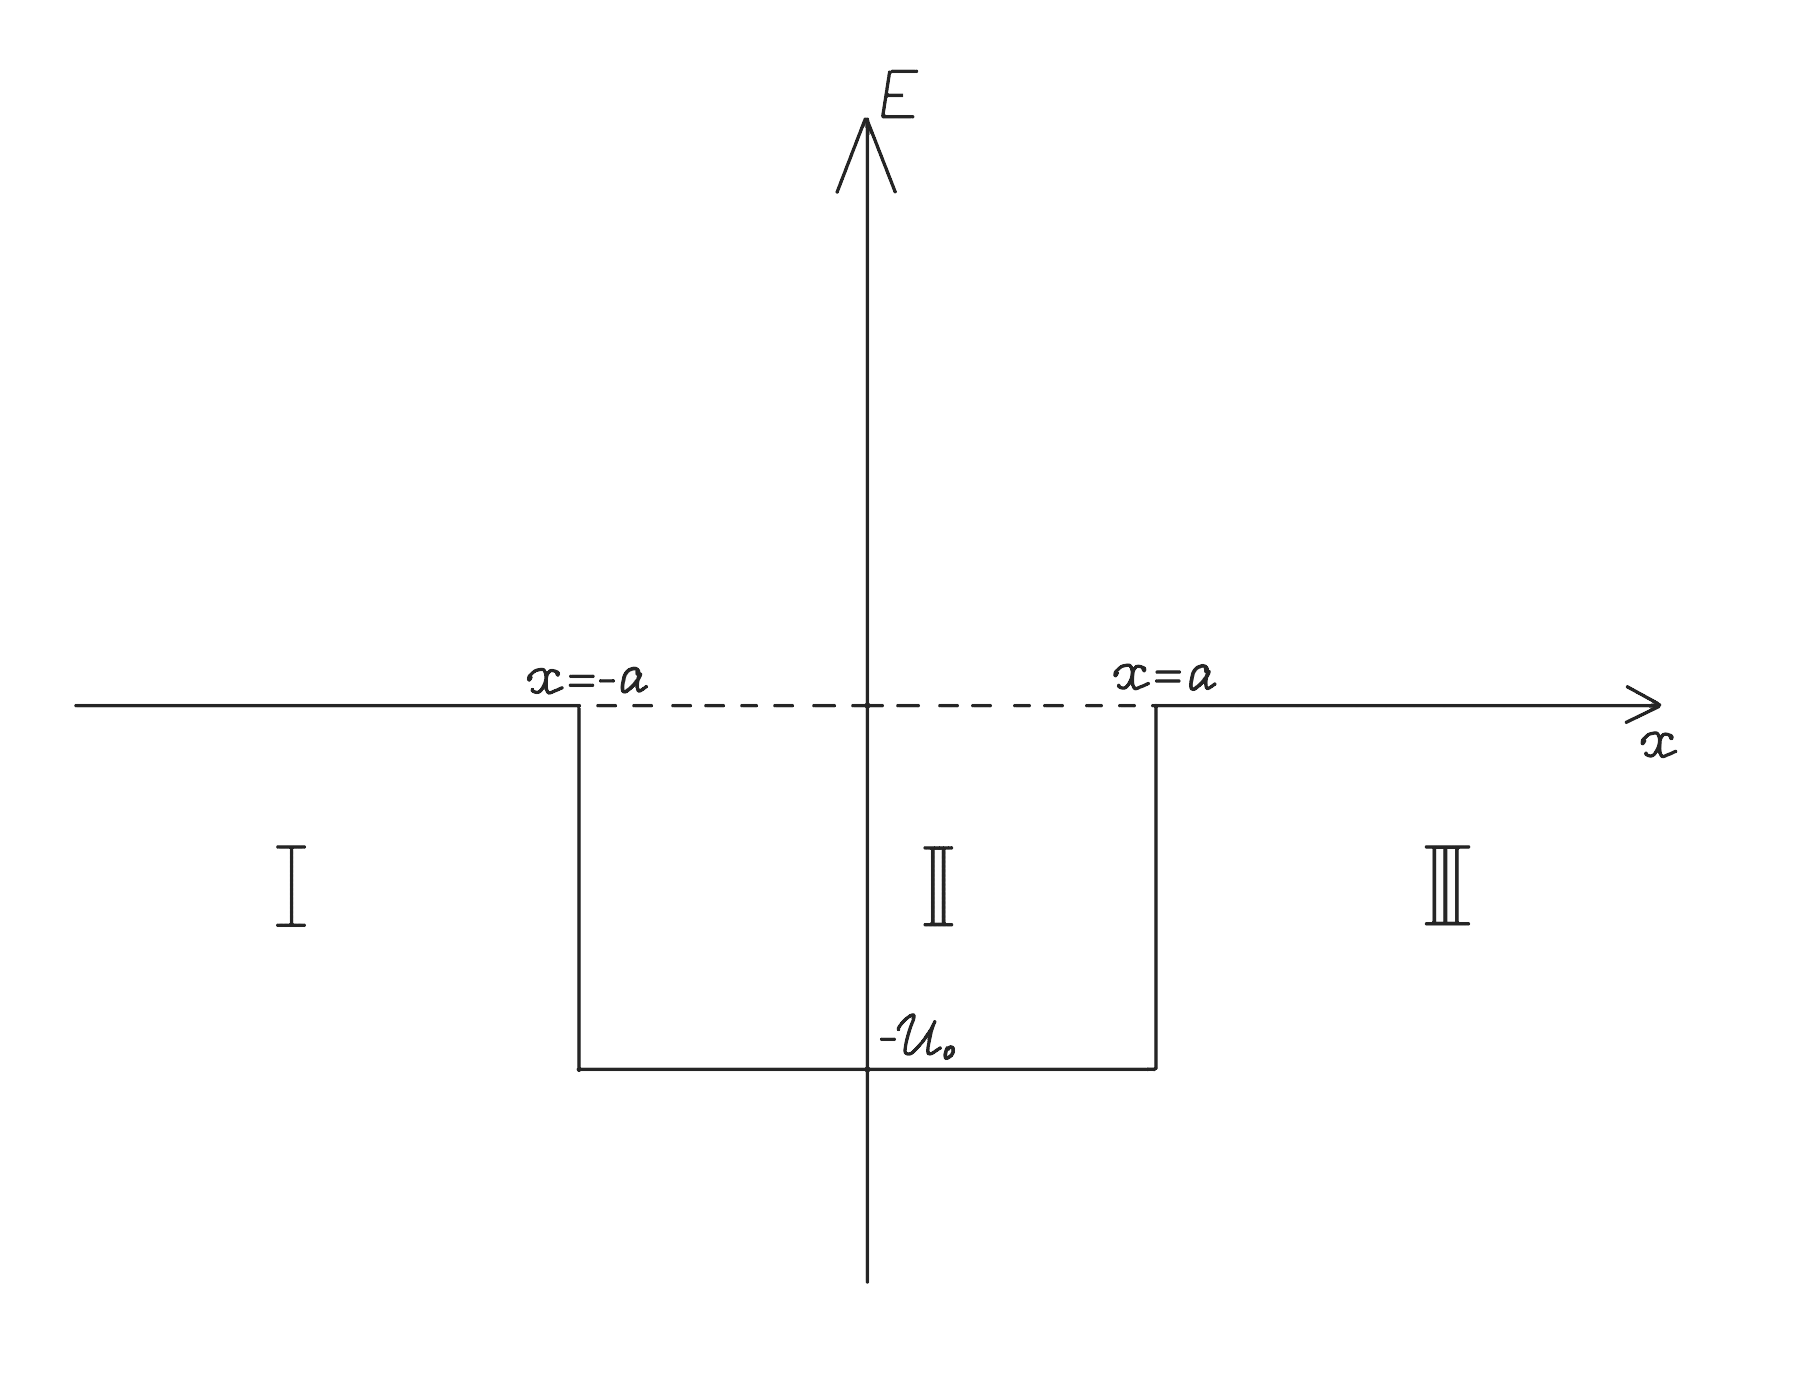
\includegraphics[scale=0.3]{class 3/images/hole.png}
\caption{Потенциальная симметричная прямоугольная яма}
\label{fig 3.1}
\end{figure}\\
Выпишем одномерное стационарное уравнение Шрёдингера:
\[
U(x)\psi(x) - \frac{\hbar^2}{2m}\psi''(x) = E\psi(x).
\]
Перепишем его, чтобы в правой части остался только 0:
\[
\psi''(x) + \frac{2m}{\hbar^2}(E-U)\psi(x) = 0
\]
Теперь давайте по отдельности рассмотрим каждую из трёх областей. В первой области (т.е. в области $x <-a$) потенциальная энергия нулевая. Так как мы рассматриваем случай финитного движения, энергия частицы меньше нуля. В классическом случае мы бы с уверенностью сказали, что в этой области частица присутствовать не может. Но в квантовой механике не всё так гладко. Давайте решим стационарное уравнение Шрёдингера для этого случая:
\[
\psi_I'' - \kappa^2\psi_I = 0, \quad \kappa^2 = \frac{2m}{\hbar^2}|E|
\]
Энергию мы берём по модулю, потому что она отрицательная, а $\kappa$ в квадрате. Это гармоническое уравнение, только с минусом. Решение такого уравнения известно и выражается в виде суммы двух экспонент с разными знаками:
\[
\psi_I(x) = Ae^{\kappa x} + \widetilde{A}e^{-\kappa x}
\]
Оказывается, что второй член из этого уравнения выпадает. Это связанно с условием нормировки -- чтобы волновая функция при $x \rightarrow -\infty$ не уходила на бесконечность. Тогда мы видим, что волновая функция для первой области имеет следующий вид:
\[
\psi_I(x) = Ae^{\kappa x},
\]
то есть функция затухает экспоненциально и на минус бесконечности уходит в ноль.

Думаю, понятно, что для третьей области решение будет аналогично. Для тренировки можете проделать все выкладки самостоятельно, я же выпишу только ответ:
\[
\psi_{III}(x) = De^{-\kappa x}
\]
Теперь выпишем уравнение для второй области:
\[
\psi_{II}'' + k^2\psi_{II} = 0, \quad k^2 = \frac{2m}{\hbar^2}(U_0 - |E|)
\]
Соответственно, решение для него
\[
\psi_{II}(x) = B\cos kx + C\sin kx
\]

Для нахождения констант воспользуемся важным теоретическим фактом о том, что если операторы коммутируют, то их собственные функции совпадают. Далее, исходя из симметрии задачи (U(x) = U(-x)), понимаем, что оператор инверсии коммутирует с гамильтонианом:
\[
[\hat{H}, \hat{I}] = [U(x) + \frac{\hat{p}^2}{2m}, \hat{I}] = [U(x), \hat{I}] + [\hat{p}^2, \hat{I}] = 0
\]
Значит, можно искать собственные функции гамильтониана как собственные функции оператора инверсии. Но мы знаем, что для оператора инверсии собственные функции обладают определенной чётностью. Тогда найдём чётные и нечётные волновые функции нашей задачи:
\[
\psi_+ =
\begin{cases}
    Ae^{\kappa x}& x < -a,\\
    B \cos kx & -a < x < a,\\
    Ae^{-\kappa x}& x > a
\end{cases}\quad
\psi_- =
\begin{cases}
    -De^{\kappa x}& x < -a,\\
    C \sin kx & -a < x < a,\\
    De^{-\kappa x}& x > a
\end{cases}
\]
Думаю, понятно, откуда взялись функции с синусом и косинусом. Чуть менее понятно может быть с оставшимися функциями. Они связаны с самим определением четной функции: $Ae^{\kappa x}$ есть у нас из решения, нам нужно составить такую функцию, которая при изменении знака икс не будет менять знак выражения. Получается $Ae^{-\kappa x}$. То же самое для второго: $De^{-\kappa x}$ есть, $-De^{\kappa x}$ мы дополняем для нечетности функции.

Рассмотрим условия на волновую функцию. Пока что она не определена на границах. То есть нужно ввести условия сшивки. Их мы берем из физического смысла волновой функции, а именно:
\[
\psi(x) - \text{непрерывна},\; \frac{\psi'(x)}{\psi(x)} - \text{непрерывна}
\]
Из этих условий ``сошьём'' границы для чётных и нечётных функций отдельно. Так как потенциал симметричен, достаточно рассмотреть только одну границу. 
\[
\frac{\psi'_+(x)}{\psi_+(x)}\bigg|_{x=a-0} = \frac{\psi'_+(x)}{\psi_+(x)}\bigg|_{x=a+0} = \frac{-Bk\sin ka}{B\cos ka} = \frac{-\kappa A e^{-\kappa a}}{Ae^{-\kappa a}} =>
\]
\[
k\tg ka = \kappa
\]
Для нечётных:
\[
\frac{\psi'_-(x)}{\psi_-(x)}\bigg|_{x=a-0} = \frac{\psi'_-(x)}{\psi_-(x)}\bigg|_{x=a+0} = \frac{Ck\cos ka}{C\sin ka} = \frac{-\kappa D e^{-\kappa a}}{De^{-\kappa a}} =>
\]
\[
k\ctg ka = -\kappa
\]
Ещё немного повертим выражение и придём к итоговому, красивому виду
\[
(\kappa a)^2 = (k_0a)^2 - (ka)^2, \; \text{где} \;k_0^2 = k^2 + \kappa^2 =>  
\]
\[
=> \kappa a = \sqrt{(k_0a)^2 - (ka)^2} => ka\tg ka = \sqrt{(k_0a)^2 - (ka)^2} =>
\]
\[
=> \tg ka = \sqrt{\frac{(k_0a)^2}{(ka)^2} - 1}
\]
\[
\tg^2 ka = \frac{1}{\cos^2 ka} - 1 =>
=> \frac{1}{\cos^2 ka} - 1 = \frac{(k_0 a)^2}{(ka)^2} - 1 => \cos^2 ka = \frac{(ka)^2}{(k_0 a)^2} =>
\]
\[
=> |\cos ka| = \frac{ka}{k_0a}, \; \tg ka>0
\]
Проделав аналогичные вычисления для нечётных функций, в итоге получаем компактное выражение
\[
\begin{cases}
   |\cos ka| = \frac{ka}{k_0a},& \tg ka>0 \\
   |\sin ka| = \frac{ka}{k_0a},& \tg ka<0 \\
\end{cases}
\]
У нас получаются трансцендентные уравнения. Т.е. просто выразить какую-либо величину из этого уравнения – сложно, или даже нереально. Мы можем только проанализировать его. Например, графически.
\begin{figure}[!h]
  \centering
  \subfloat[График для чётных функций. Выделенные области удовлетворяют условию $\tg ka > 0$]{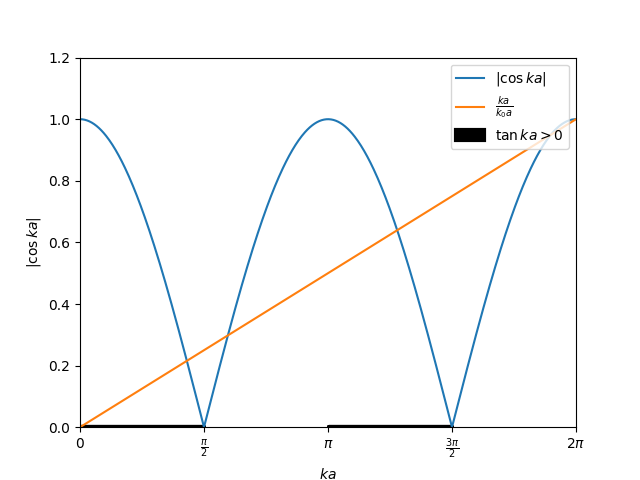
\includegraphics[scale=0.5]{class 3/images/even.png}}
  \hfill
  \subfloat[График для нечётных функций. Выделенные области удовлетворяют условию $\tg ka < 0$]{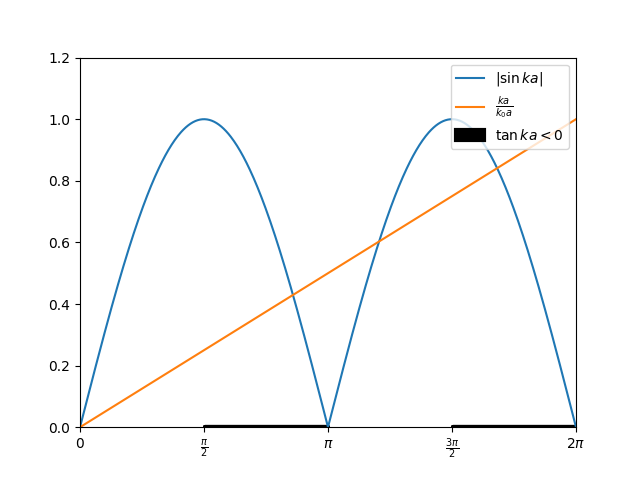
\includegraphics[scale=0.5]{class 3/images/odd.png}}
  \caption{}
\end{figure}
\\
Что мы можем вынести из этих графиков? Для чётных функций видно, что решение существует при любом положительном $k_0a$. Так как этот параметр отвечает параметрам задачи, получается, что при любой глубине ямы у нас существует хотя бы одно чётное решение. В то же время, из графика нечётных функций достаём следующее условие существования решений: $k_0a>\frac{\pi}{2}$. Можно легко проверить, что чётные и нечётные решения чередуется. Формулы для количества решений:
\[
[\frac{k_0a}{\pi}] + 1 = N_+,\quad[\frac{k_0a}{\pi/2}] = N_-
\]
Теперь найдём коэффициенты A и B из неиспользованного условия непрерывности:
\[
\psi_+(a-0) = \psi_+(a+0) => A = Be^{\kappa a}\cos ka
\]

\[
\braket{\psi_+} = 1 => 2 * (\int\limits_0^a |B|^2\cos^2 kx dx + \int\limits_a^\infty |A|^2e^{-2\kappa(x)} dx) = 1 =>
\]
\[
 => 2 *|B|^2 (\int\limits_0^a \cos^2 kx dx + \int\limits_a^{+\infty }\cos^2 kae^{-2\kappa(x-a)} dx) = 1 =>
\]
\[
=> |B|^2 = (a + \frac{\sin 2ka}{2k} + \frac{\cos^2 ka}{\kappa})^{-1} 
\]
Проделав ту же самую процедуру с D и C, получим
\[
D = Ce^{\kappa a}\sin ka, \quad |C|^2 = (a - \frac{\sin 2ka}{2k} + \frac{\sin^2 ka}{\kappa})^{-1}
\]
Всё, основную часть мы проанализировали, волновые функции и уровни энергии получили. Оставшиеся вопросы будут обсуждены на очном семинаре и предоставляются тем, кто его пропустил, в виде \sout{наказания} упражнения.

На следующем семинаре продолжим разбирать задачи, связанные с одномерным потенциалом и уравнением Шрёдингера.
\csquare{darklavender}
    \newpage
    \begin{center}
    \section{Семинар IV}
\end{center}
\subsection{Решение задач на потенциальные ямы}
\excersize{Упражение №13}{darklavender}
\begin{center}
    \textit{Найдите уровни энергии и волновые функции стационарных состояний для частицы m в одномерной потенциальной яме следующего вида:}
    \[
    U(x) =
    \begin{cases}
    +\infty,& x<0,\\
    -U_0,& 0<x<a,\\
    0,& x>a
    \end{cases}
    \]
    \textit{Что здесь можно сказать о связанных состояниях при фиксированном $a$ и $U_0 \rightarrow 0$?}
\end{center}
На рисунке \ref{fig 4.1} снова можем увидеть потенциальную яму, но уже с бесконечной стенкой. Давайте обсудим, как от этого изменится задача.
\begin{figure}[h!]
\centering
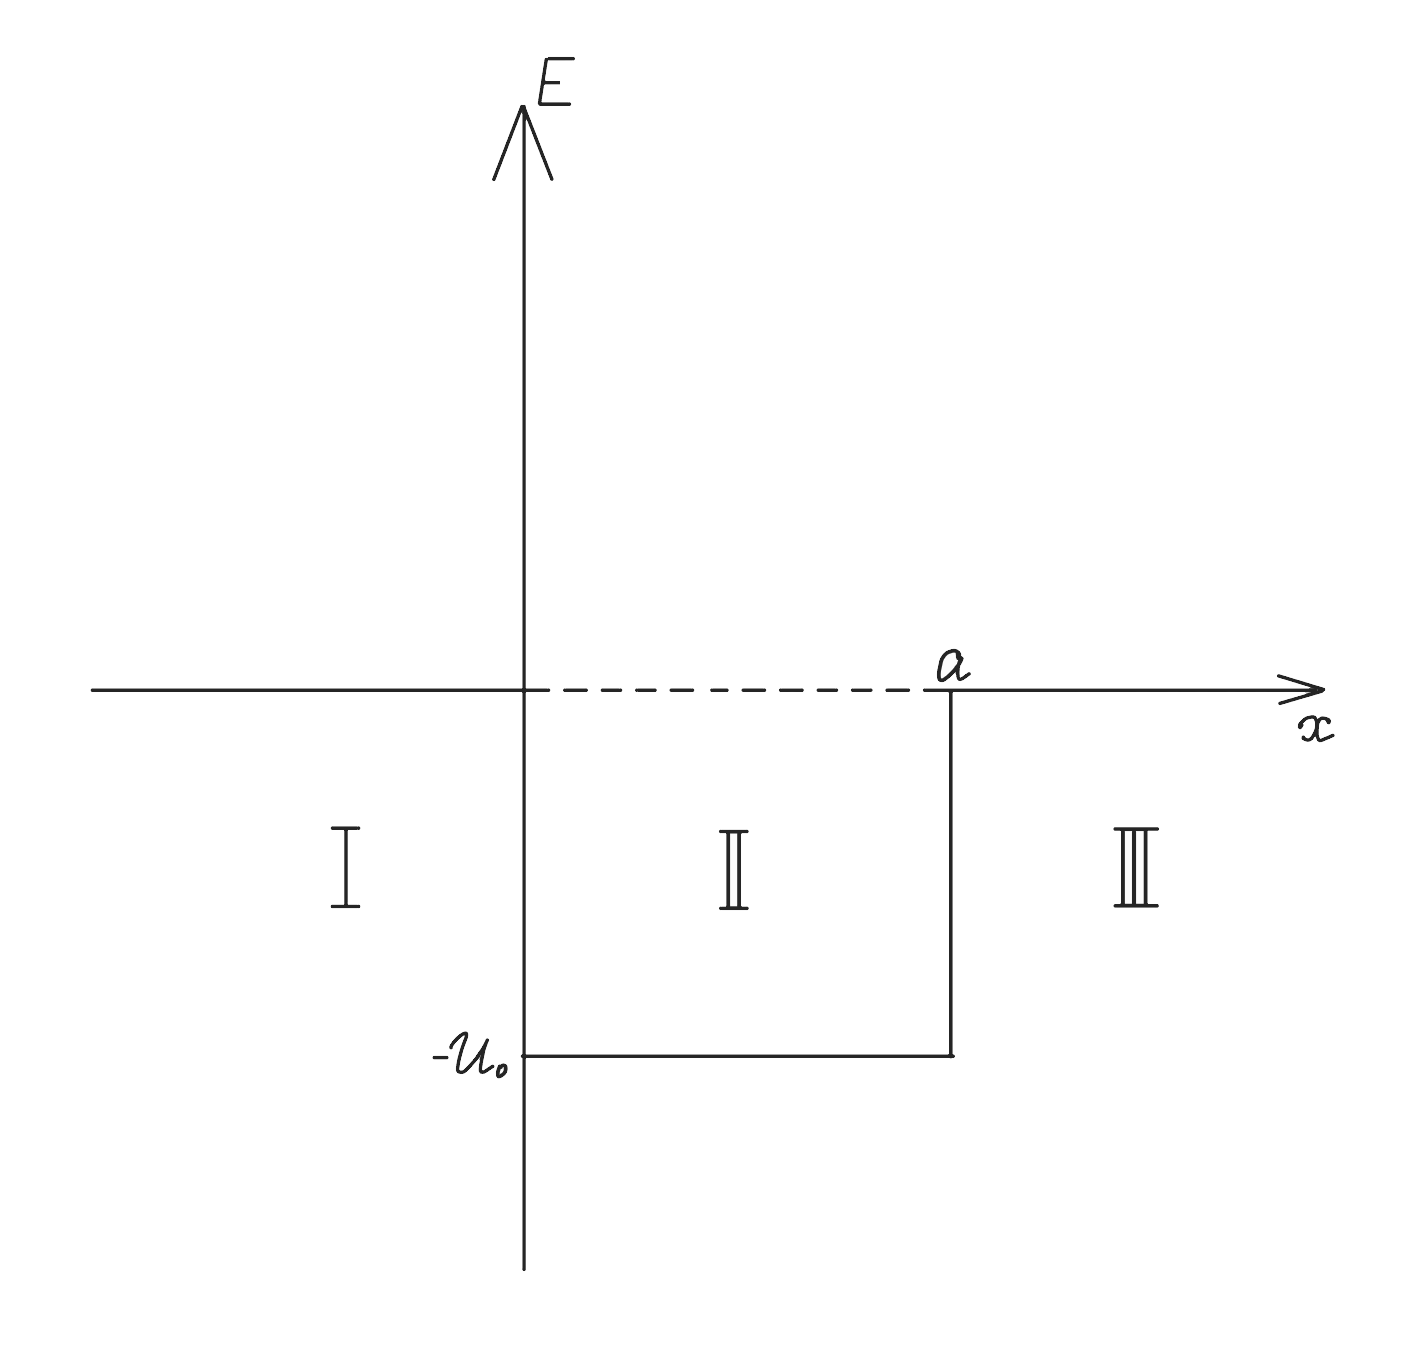
\includegraphics[scale=0.27]{class 4/images/half-inf hole.png}
\caption{Потенциальная яма с одной бесконечной стенкой}
\label{fig 4.1}
\end{figure}\\
Запишем уравнение Шрёдингера:
\[
\psi'' + \frac{2m}{\hbar^2}(E-U(x))\psi = 0 
\]
Не трудно заметить, что правая часть очень похожа на задачу 1.1. Рассмотрим, что происходит у левой стенки. Мы считаем, что, как и на бесконечности в случае обычной ямы, частица не может пройти через такой барьер, т.е. $\psi(x) = 0$ при $x\leq 0$. Тогда, из условия непрерывности, получим условия сшивки (напоминаю, что решения в области $II$ имеет вид $\psi(x) = \widetilde{A}\cos kx + A\sin kx$):
\[
\psi(0) = \widetilde{A} = 0 => \psi(x) =
\begin{cases}
    0,& x < 0,\\
    A\sin kx,& 0<x<a,\\
    Be^{-\kappa x},& x>a
\end{cases}
\]
Я думаю, уже видно, что мы можем переписать это через нечетные волновые функции из задачи 1.1. Тогда получим:
\[
\psi(x) =
\begin{cases}
    0,& x\leq 0,\\
    \sqrt{2}\psi_-(x), x>0
\end{cases}
\]
Коэффициент $\sqrt{2}$ появился из следующих соображений: волновая функция, относительно первой задачи, уменьшилась вдвое, значит нужно её перенормировать. Если хотите в этом убедиться, подставьте вместо корня из двух коэффициент C и решите уравнение $\int\limits_0^{+\infty}|\psi(x)|^2 = 1$. Получится то же самое!
\csquare{darklavender}

\excersize{Упражнение №14}{rosewood}
\begin{center}
    \textit{Частица массы m совершает финитное движение в одномерной модельной потенциальной яме, вид которой может быть представлен $\delta$-функцией:}
    \[
    U(x) = -\frac{\hbar^2\kappa_0}{m}\delta(x),
    \]
    \textit{где $\kappa_0$ - параметр ямы. Покажите, что в этой яме имеется только одно связанное состояние и найдите энергию и волновую функцию частицы связанного состояния в координатном представлении. Вычислите $\langle x\rangle,\,\langle p\rangle,\,\langle (\Delta x)^2\rangle$ и $\langle (\Delta p)^2\rangle$ в этом состоянии}
\end{center}
Не переживайте, дельта функция только выглядит страшно. На деле у нас получается примерно такой рисунок:
\begin{figure}[h!]
\centering
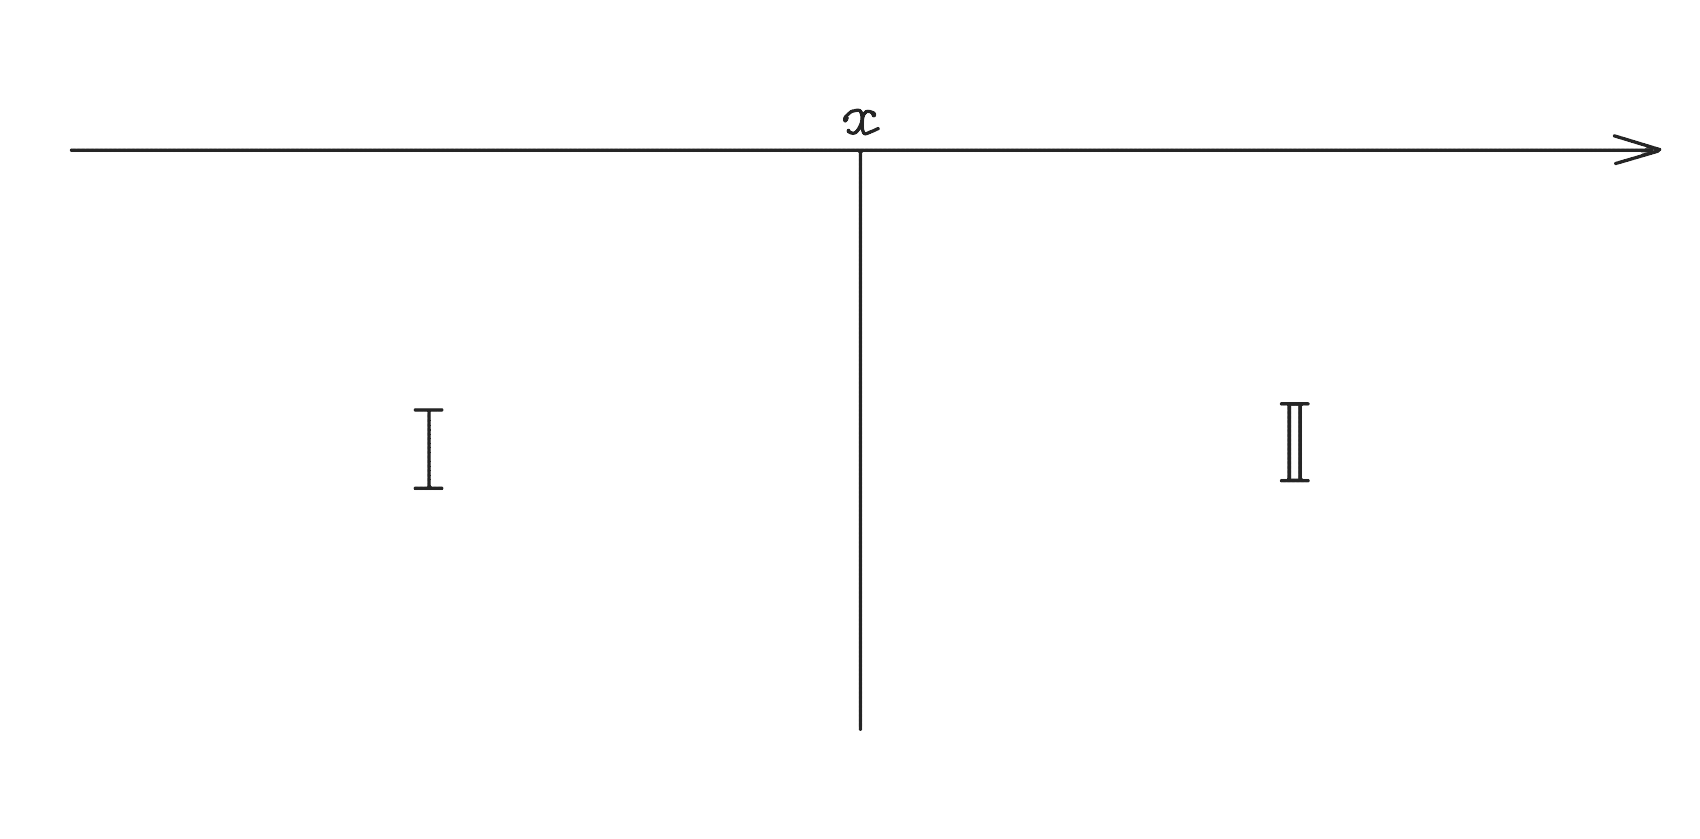
\includegraphics[scale=0.26]{class 4/images/delta hole.png}
\caption{Потенциальная дельта яма}
\label{fig 4.2}
\end{figure}\\
Введём уже знакомую нам величину $\kappa^2 = \frac{2m|E|}{\hbar^2}$ и запишем уравнение Шрёдингера:
\[
\psi''(x) - (\kappa^2 - 2\kappa_0\delta(x))\psi(x) = 0
\]
Решение для областей $I$ и $II$ мы уже сто раз нашли, так что сразу выпишу их:
\[
\begin{cases}
    \psi_I(x) = Ae^{\kappa x}\\
    \psi_{II}(x) = Be^{-\kappa x}\\
\end{cases}
\]
Волновая функция в нуле должна быть непрерывна: 
\begin{equation}
\psi(+0) = \psi(-0)    
\end{equation}

Производная же будет разрывна (из-за дельта-функции). Доопределим разрыв, проинтегрировав уравнение Шрёдингера с пределами от $-\epsilon$ до $\epsilon$, где $\epsilon \rightarrow 0$. Получим:
\[
\int\limits_{-\epsilon}^{\epsilon}\psi''(x)dx = \int\limits_{-\epsilon}^{\epsilon}\psi(x)\kappa^2 dx - \int\limits_{-\epsilon}^{\epsilon}2\kappa_0\delta(x)\psi(x) dx =>
\]
\[
    \psi'(+0) - \psi'(-0) = -2\kappa_0\psi(0)    
\]
Второй интеграл равен нулю, так как по теореме о среднем этот интеграл равен $\mu2*\epsilon\psi(0)$, но $\epsilon \rightarrow 0$.

Выпишем волновые функции и воспользуемся полученными условиями:
\[
\begin{cases}
    \psi_I(x) = Ae^{\kappa x}\\
    \psi_{II}(x) = Be^{-\kappa x}\\
    \psi(+0) = \psi(-0)
\end{cases}
=> A = B => \psi(x) = Ae^{-\kappa|x|}
\]
Подставим условие на производную и получим:
\[
-A\kappa - A\kappa = -2A\kappa_0 => \kappa = \kappa_0 => 
\]
\[
E_0 = - \frac{\hbar^2 \kappa_0^2}{2m}
\]
Выходит, что в дельта яме только один уровень энергии. Найдём коэффициент A из условия нормировки:
\[
\int\limits_{-\infty}^{+\infty} |\psi(x)|^2 dx = A^2\int\limits_{-\infty}^{+\infty} e^{-2\kappa |x|} = A^2\left[\int\limits_{-\infty}^0 e^{2\kappa x}\right] + \int\limits_0^{+\infty} e^{-2\kappa x}) = A^2\left[ \frac{1}{2\kappa}(1 - 0) - \frac{1}{2\kappa}(0-1)\right] = 
\]
\[
= \frac{A^2}{\kappa} = 1 \; => \; A = \sqrt{\kappa}
\]
Наконец, запишем итоговую волновую функцию:
\[
\psi(x) = \sqrt{\kappa_0}e^{-\kappa_0 x}
\]
Найдём среднее значение координаты и импульса. Дисперсию читателю представляется найти самостоятельно в виде упражнения.
\[
\langle x \rangle = \int\psi^*x\psi dx = 0, \text{т.к. $\psi$ - чётная}
\]
\[
\langle p \rangle = \int\psi^*(-i\hbar\frac{\partial}{\partial x}\psi) dx = -i\hbar\kappa_0^2\int e^{-\kappa_0|x|}(-e^{-\kappa_0|x|}sign(x)) dx = 0
\]
\csquare{darklavender}
\excersize{Упражнение №15}{darklavender}
\begin{center}
    \textit{Частица массы m совершает финитное движение в одномерном потенциальном поле вида:}
    \[
    U(x) = -\frac{\hbar^2\kappa_0}{m}(\delta(x+a) + \delta(x-a)),
    \]
    \textit{где $\kappa_0$ - параметр ямы. Найдите энергии уровней и волновые функции стационарных состояний. Как зависит число связанных состояний от параметров $a$ и $\kappa_0$?}
    
    \textit{Покажите, что в случае $\kappa_0a \gg 1$ связанные состояния представляют собой дублет близко расположенных уровней. В этом же пределе $\kappa_0a\gg1$ найдите вероятность нахождения частицы в момент $t$ в правой яме ($x=a$), если при $t=0$ она находилась в левой яме ($x=-a$)}
\end{center}
На рисунке \ref{fig 4.3} можно увидеть ситуацию, описываемую в задаче.
\begin{figure}[h!]
\centering
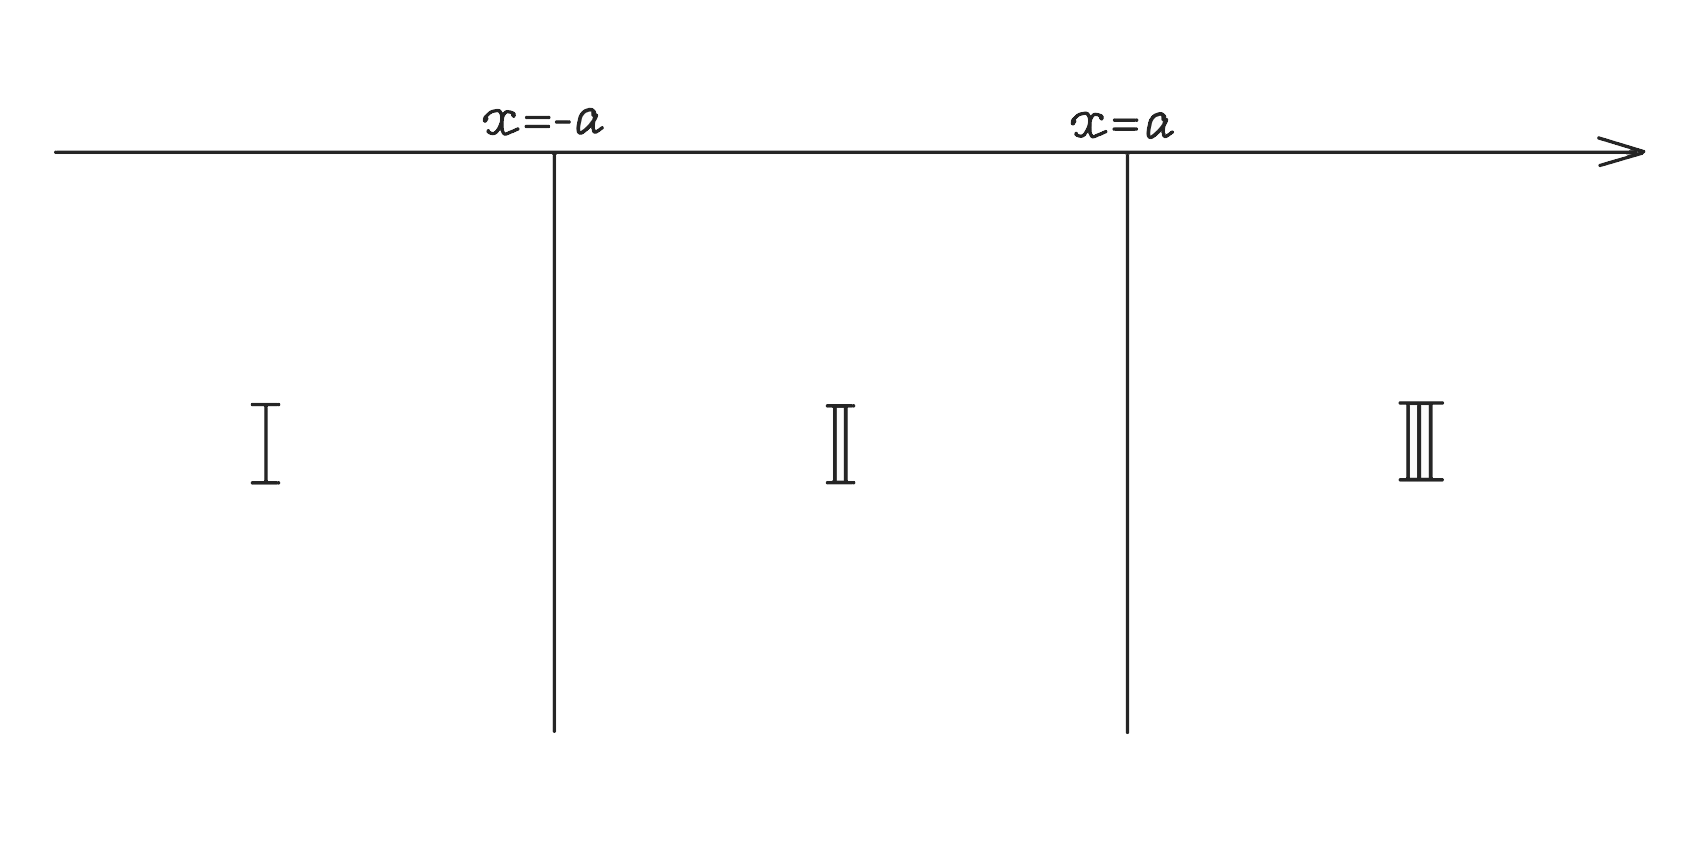
\includegraphics[scale=0.27]{class 4/images/two delta hole.png}
\caption{Две потенциальные дельта ямы}
\label{fig 4.3}
\end{figure}

Давайте для начала рассмотрим области вне дельта ям. Ясно (если нет, проделайте те же самые выкладки, что мы делали в задаче 1.1), что решением здесь будут так же четные и нечетные функции следующего вида:
\[
\psi_+ =
\begin{cases}
    Ae^{\kappa x}& x < -a,\\
    B\,ch\,\kappa x & -a < x < a,\\
    Ae^{-\kappa x}& x > a
\end{cases}\quad
\psi_- =
\begin{cases}
    -De^{\kappa x}& x < -a,\\
    C\, sh\, \kappa x & -a < x < a,\\
    De^{-\kappa x}& x > a
\end{cases}
\]
Тригонометрические функции превратились в гиперболические из-за отсутствия отрицательного потенциала между ямами. Далее, приведём к форме, удобной для анализа (в очередной раз графического). Для этого вновь воспользуемся условиями ``сшивки'', а именно разрывом производной и непрерывностью, полученной в прошлой задаче:
\[
\begin{cases}
\psi'(a+0) - \psi'(a-0) = -2\kappa_0\psi(a)\\
\psi(a+0) = \psi(a-0)    
\end{cases}
\]
Проведем все необходимые преобразования для чётных функций (для нечётных аналогично):
\[
Ae^{-\kappa a} = B\,ch\,ka => B = \frac{1}{2}A(e^{2\kappa a} + 1)
\]
Из первого уравнения получим:
\[
-A\kappa e^{-\kappa a} - B\kappa\,\sh\,\kappa a = -2\kappa_0 Be^{-\kappa a}
\]
Подставляя $B$ и проведя все сокращения, получим итоговое выражение:
\begin{equation}
    \frac{\kappa a}{\kappa_0 a} = 1 + e^{-2\kappa a}
\end{equation}
Для нечетного же случая:
\begin{equation}
    \frac{\kappa a}{\kappa_0 a} = 1 - e^{-2\kappa a}
\end{equation}
Давайте опять сделаем красивый (или не очень) график и обсудим его.
\begin{figure}[h!]
\centering
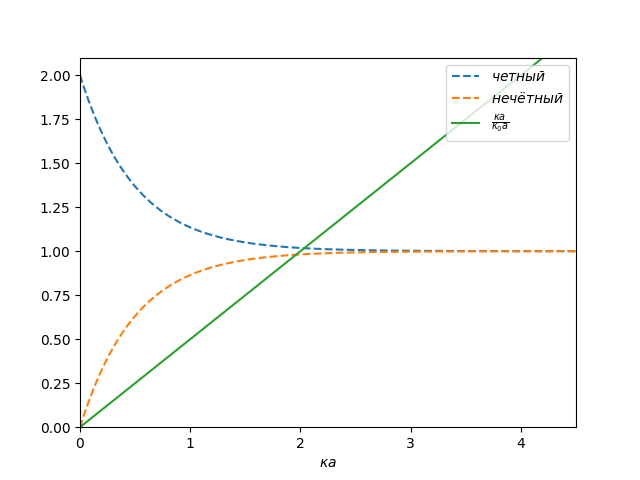
\includegraphics[scale=0.5]{class 4/images/delta.png}
\caption{График для нечетных и четных функций}
\label{fig 4.4}
\end{figure}

Два важных замечания по графику:
\begin{enumerate}
    \item Видно, что чётное решение, в отличие от нечётного, существует всегда. Нечётное решение же существует только при $\kappa_0a\geq 1/2$.
    \item При $\kappa_0a\gg 1$ решения почти неразличимы. Однако, если $\kappa a \ll 1$, то у нас остаётся одна дельта яма с удвоенным $\kappa_0$.
\end{enumerate}
Найдём коэффициенты для собственных функций (так же, как в задаче 1.1).
\[
|A|^2 =  (a + \frac{sh\, 2\kappa a}{2\kappa} + \frac{ch ^2\,\kappa a}{\kappa})^{-1},\; B = Ae^{\kappa a}\,ch\,\kappa a
\]
\[
|D|^2 = (-a + \frac{sh\, 2\kappa a}{2\kappa} + \frac{sh ^2\,\kappa a}{\kappa})^{-1},\;C = De^{\kappa a}\,sh\,\kappa a
\]
Задача на вероятность перехода будет решена на семинаре :)
\csquare{darklavender}

\excersize{Упражнение №16}{darklavender}
\begin{center}
    \textit{Частица массы m движется в одномерном периодическом поле вида}
    \[
    U(x) = -\frac{\hbar^2\kappa_0}{m}\sum\limits_{n=-\infty}^{n = +\infty}\delta(x-na),
    \]
    \textit{где $\kappa_0$ и $a$ - параметры потенциала. Исследуйте, при каких отрицательных и положительных энергиях $E$ частицы такое движение возможно. Покажите, что имеются зоны ``разрешенных'' и ``запрещенных'' энергий.}
    \textit{Исследуйте, что происходит с шириной зон в предельных случаях $\kappa_0a\gg1$ (сильная связь) и $\kappa_0a\ll1$(слабая связь).}
    
\end{center}
Мы решили задачу на одну яму, на две ямы, следующий логичный шаг - решить задачу на \sout{три} бесконечность дельта ям.

Писать условие сшивки для бесконечного количества ям не самая приятная задача и предоставляется читателю в качестве упражнения на дом. Мы же пойдём другим путём, заметив важную особенность задачи. Посмотрев на рисунок \ref{fig 4.5} и на дельта потенциал, становится понятно, что задача a-периодична. А какой оператор у нас двигает частицу на a? Правильно, оператор трансляции $\hat{T}_a$. Проверим, коммутирует ли гамильтониан с оператором трансляции:
\[
[\hat{H}, \hat{T}_a] = [u(x), \hat{T}_a] + [\hat{p}^2, \hat{T}_a] = [\sum\delta(x-na), \hat{T}_a] + [\hat{p}^2, e^{-\frac{i}{\hbar}a\hat{p}}] = 0.
\]
Значит, мы можем искать собственные функции гамильтониана в виде $e^{ikx}\phi(x)$, где $\phi(x + a) = \phi(x)$. Помимо этого, нам достаточно написать условия сшивки для зоны I и зоны II. Выпишем действие оператора трансляции отдельно, оно нам ещё понадобится:
\[
\hat{T}_a\psi(x) = \psi(x+a) = e^{ia\kappa}\psi(x)
\]
\begin{figure}[h!]
\centering
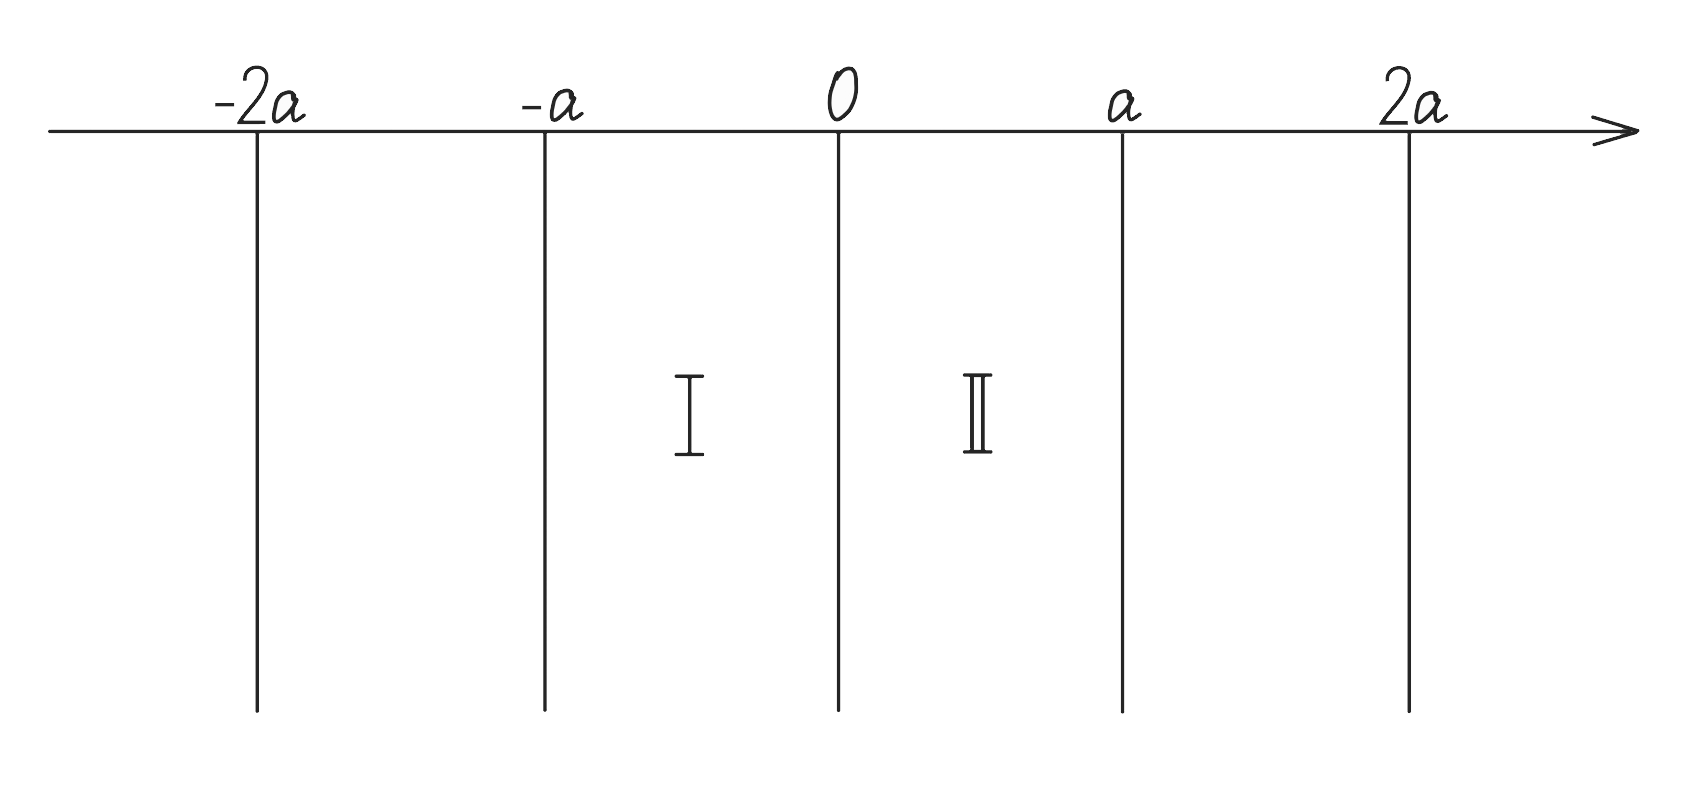
\includegraphics[scale=0.27]{class 4/images/inf delta hole.png}
\caption{Бесконечные дельта ямы}
\label{fig 4.5}
\end{figure}

Напишем уравнение Шрёдингера для зоны I и зоны II без учёта дельта потенциала и с положительной энергией (!):
\[
\psi''(x) + \kappa^2\psi(x) = 0, \; \kappa^2 = \frac{2m}{\hbar^2}E
\]
Решение этого уравнение мы запишем в следующем виде:
\[
\psi_I(x) = Ae^{i\kappa x} + Be^{-i\kappa x}
\]
\[
\psi_{II}(x) = e^{ika}\left[Ae^{i\kappa(x-a)} + Be^{-i\kappa(x-a)}\right]
\]
Второе уравнение мы получили, не решая уравнение Шрёдингера, а сдвинув его во вторую область с помощью оператора трансляции. Таким образом, мы смогли выразить оба наших решения через одни коэффициенты A и B.

Теперь запишем условия сшивки. Напомню, что $\psi_I(0) = \psi_{II}(0)$ и $\psi'_{II}(0) - \psi'_I(0) = -2\kappa_0\psi(0)$. Тогда
\[
\begin{cases}
A + B = e^{ika}\left[Ae^{-i\kappa a} + Be^{i\kappa a}\right]\\
e^{ika}(Ae^{-i\kappa a}i\kappa - Be^{i\kappa a}i\kappa) - Ai\kappa + Bi\kappa = -2\kappa_0(A+B)
\end{cases}
\]
Чтобы у системы уравнений было нетривиальное решение, необходимо, чтобы определитель матрицы системы был равен нулю. Давайте выпишем матрицу системы:
\[
\begin{cases}
A(1 - e^{i(k-\kappa)a}) + B(1 - e^{i(k+\kappa)a}) = 0\\
A(e^{i(k-\kappa)a}i\kappa - i\kappa + 2\kappa_0) - B(e^{i(k+\kappa)a}i\kappa - i\kappa - 2\kappa_0) = 0
\end{cases}
=>
\]
\[
\begin{vmatrix}
1 - e^{i(k-\kappa)a} & 1 - e^{i(k+\kappa)a} \\
e^{i(k-\kappa)a}i\kappa - i\kappa + 2\kappa_0 & e^{i(k+\kappa)a}i\kappa - i\kappa - 2\kappa_0
\end{vmatrix}
= 0
\]
Распишем детерминант и применим всю силу тригонометрии:
\begin{multline*}
(1 - e^{i(k-\kappa)a})(e^{i(k+\kappa)a}i\kappa - i\kappa - 2\kappa_0) - (1 - e^{i(k+\kappa)a})(e^{i(k-\kappa)a}i\kappa - i\kappa + 2\kappa_0) = \\
i\kappa - i\kappa e^{i(k-\kappa)a} - i\kappa e^{i(k+\kappa)a} + i\kappa e^{2ika} - \kappa_0 e^{i(k-\kappa)a} + \kappa_0 e^{i(k+\kappa)a} = \\
e^{ika}\left( i\kappa e^{-ika} - i\kappa e^{-i\kappa a} - i\kappa e^{i\kappa a} + i\kappa e^{ika} - \kappa_0 e^{-i\kappa a} + \kappa_0 e^{i\kappa a}\right) = \\
i\kappa\left( 2\cos ka - 2\cos\kappa a \right) + 2i\kappa_0\sin\kappa a = i\kappa\cos ka - i\kappa\cos\kappa a + i\kappa_0\sin\kappa a = 0
\end{multline*}
В итоге получим:
\[
\cos ka = \cos\kappa a - \frac{\kappa_0}{\kappa}\sin\kappa a.
\]
Проделав то же самое для отрицательной энергии, получим
\[
\cos ka = \cosh(\eta a) - \frac{\kappa_0}{\eta}\sinh(\eta a), \; \eta^2 = \frac{2m}{\hbar^2}|E|
\]
\begin{figure}[h!]
\centering
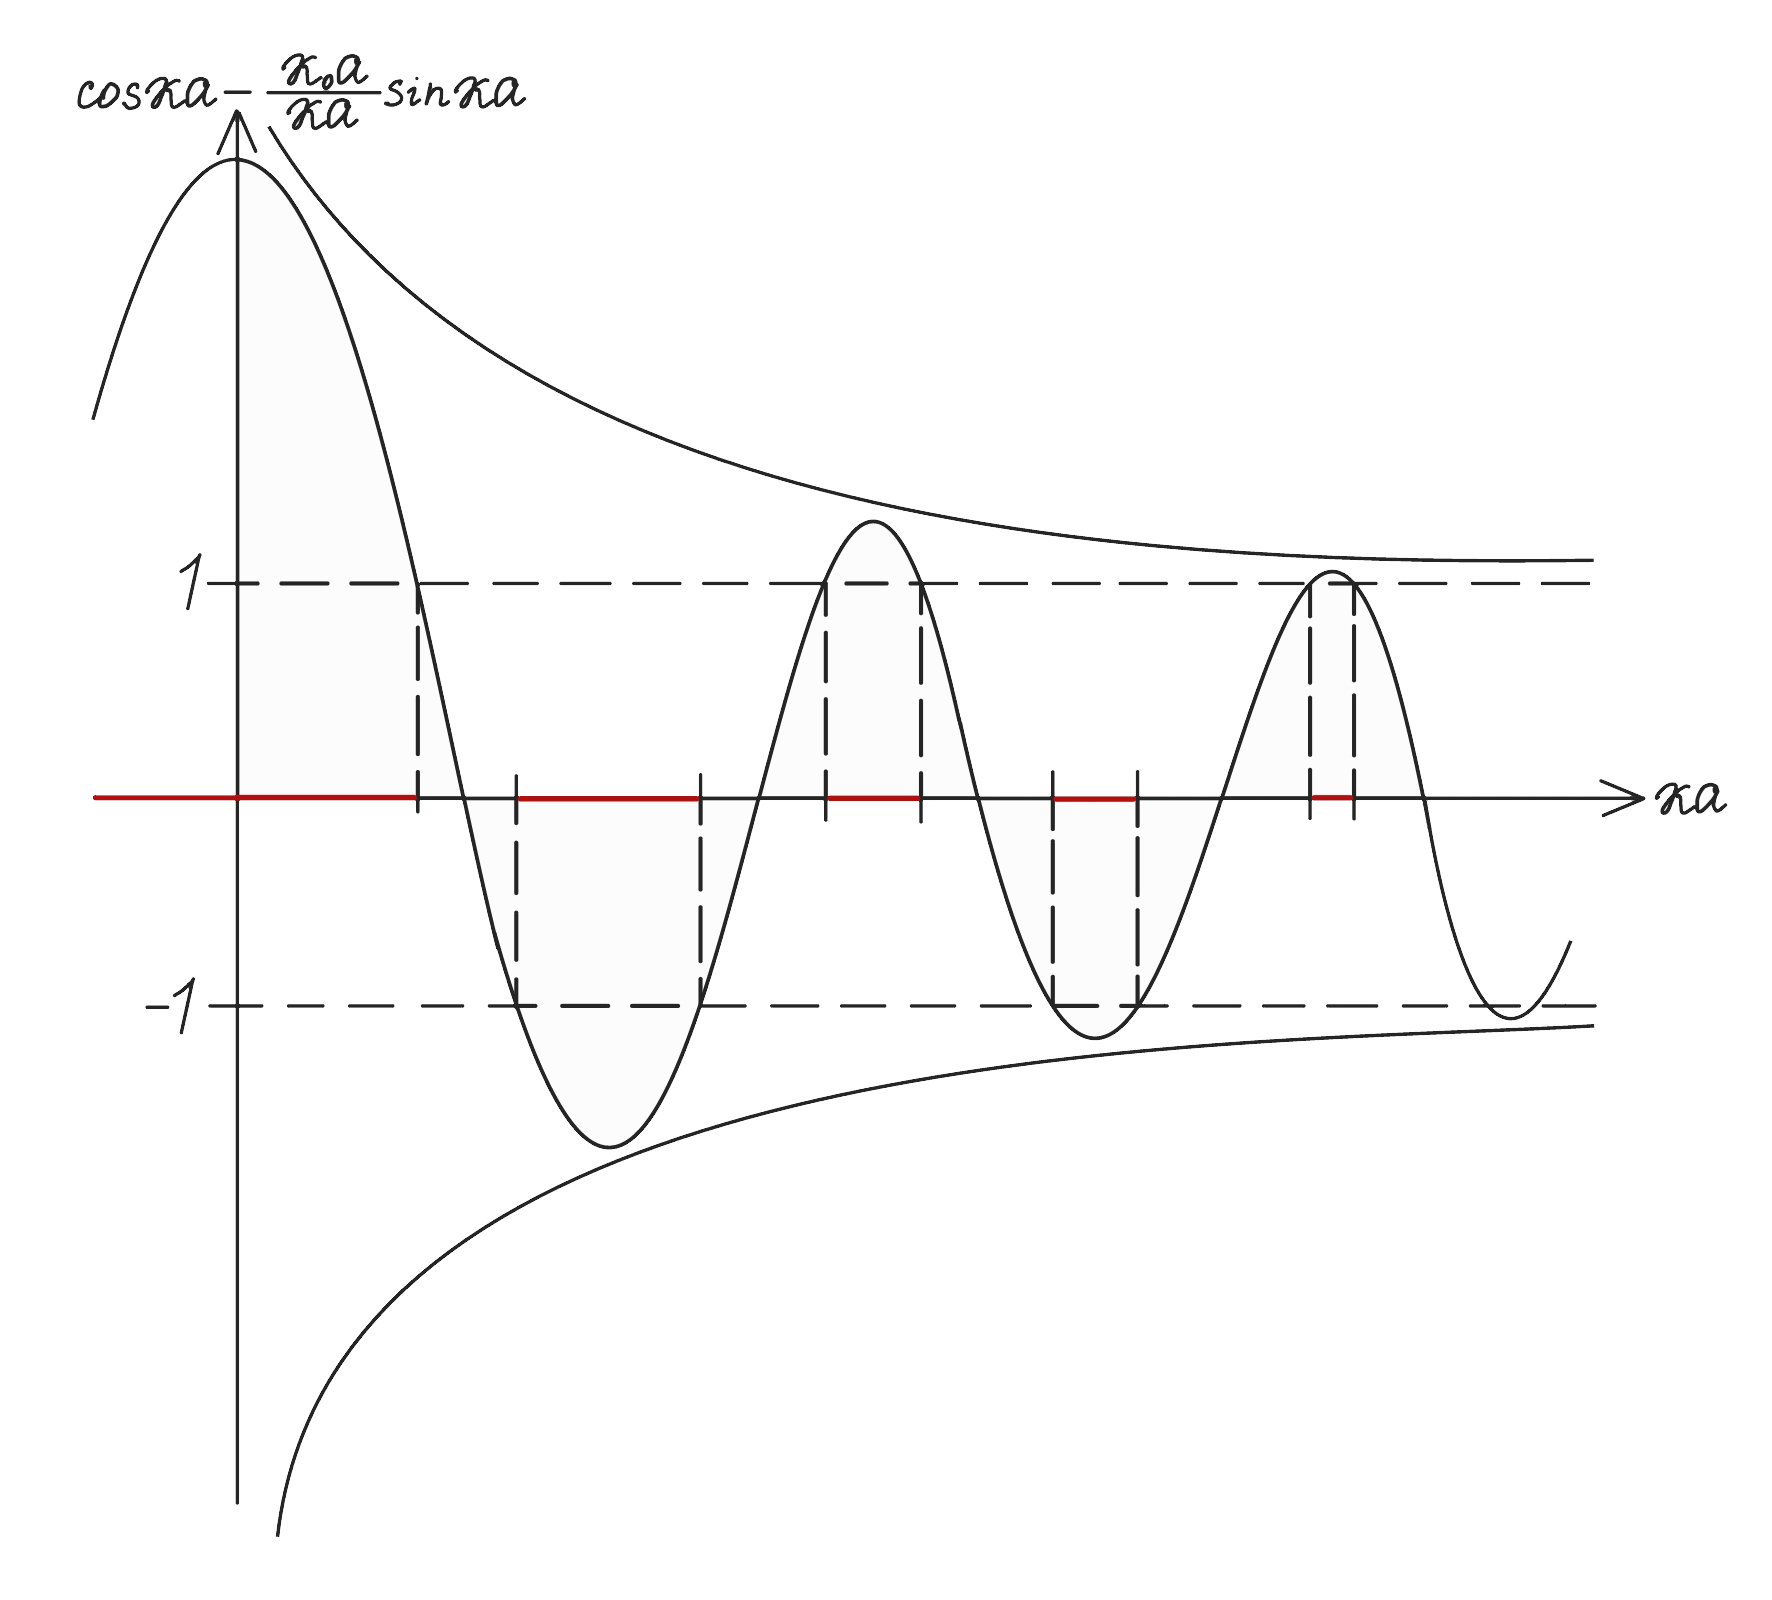
\includegraphics[scale=0.23]{class 4/images/pos energy delta.png}
\caption{График для положительных энергий}
\label{fig 4.6}
\end{figure}

Мы получили зависимость энергии ($\kappa$ или $\eta$) от квазиимпульса $k$, т.е. у нас получились дисперсионные соотношения. Проанализируем эти уравнения на графике (\ref{fig 4.6}). Так как значение k у нас действительные, косинус энергии не может выходить за пределы 1 и -1. Получается, что все зоны, когда график выходит за пределы, являются запрещёнными для энергии. И наоборот, значения внутри наших пределов будут разрешенными. Мы получили зонную структуру. Дальнейший численный анализ можно провести самостоятельно, главное, что идею мы уловили. 
\csquare{darklavender}
На следующем семинаре мы с вами решим последнюю задачу на ямы и обсудим ситуацию с барьерами.
    \newpage
    \begin{center}
    \section{Семинар V}
\end{center}
\subsection{Решение задач на потенциальные барьеры}
\excersize{Упражнение №17}{darklavender}
\begin{center}
    \textit{Получите стационарное уравнение Шрёдингера в задаче 1.4 в импульсном представлении. Найдите решение этого уравнения, описывающее связанное состояние частицы. Преобразуйте найденную волновую функцию частицы в импульсном представлении в волновую функцию в координатном представлении и удостоверьтесь в правильности ответа.}
\end{center}
Вообще, задача очень нудная, но если прорешать её самостоятельно (что я вам очень советую), то можно очень хорошо разобраться с переходами между импульсными и координатными представлениями. Напомню, что в бракет форме волновое уравнение выглядит так:
\[
i\hbar \frac{d}{dt} \ket{\psi} = \hat H \ket{\psi}
\]
Уравнение Шрёдингера из него получается путем проецирования обеих частей на вектор координаты. В нашем же случае нужно спроецировать на вектор импульса. Буду писать эту часть достаточно подробно:
\[
\bra{p} i\hbar \frac{d}{dt} \ket{\psi} = \bra{p} \hat H \ket{\psi}
\]
Раскроем оператор Гамильтона как $\hat H = \frac{\hat p^2}{2m} + U(\hat x)$ и перепишем $\bra{p}\ket{\psi}$ в виде $\psi_p$
\[
i\hbar \frac{d}{dt} \psi_p = \frac{p^2}{2m}\psi_p + \bra{p}U(\hat{x})\hat{1}_p\ket{\psi} = \frac{p^2}{2m}\psi_p + \int\bra{p}U(\hat x)\ket{p'}\psi_{p'}\;dp'.
\]
Нам необходимо вычислить матричный элемент $U(\hat{x})$ в импульсном представлении. Используем единичный оператор (только на этот раз координаты), вставляя его в наше скалярное произведение:
\[
\int\bra{p}U(\hat x)\hat{1}_x\ket{p'}\psi_{p'}\;dp' = \int \bra{p}U(\hat x)\left[\int\ket{x}\bra{x}dr\right]\ket{p'} \psi_{p'}\;dp'=
\]
\[
= \int\int U(\hat x)\bra{p}\ket{x}\bra{x}\ket{p'} \psi_{p'} dx\,dp' = \frac{1}{2\pi\hbar}\int\int U(x) e^{-\frac{i}{h}(p-p')x}\psi_{p'} dx\,dp'
\]
Подставляя его в изначальное уравнение, получим уравнение Шрёдингера в импульсном представлении:
\[
i\hbar \frac{d}{dt} \psi_p =\frac{p^2}{2m}\psi_p + \frac{1}{2\pi\hbar}\int\int U(x) e^{-\frac{i}{h}(p-p')x}\psi_{p'} dx\,dp'.
\]
Подставляя потенциальную энергию из задачи 1.4, получим:
\[
\frac{p^2}{2m}\psi_p - \frac{\kappa_0\hbar}{2\pi m}\int\int \delta(x) e^{-\frac{i}{h}(p-p')x}\psi_{p'} dx\,dp'= \frac{p^2}{2m}\psi_p - \frac{\kappa_0\hbar}{2\pi m}\int\psi_{p'} dp' =  E\psi_p
\]
Предположим, что интеграл сходится, и введём для него обозначение $I = \int \psi_{p'}dp'$. Далее, выражая энергию через $\kappa$, получим простое алгебраическое выражение на $\psi_p$:
\[
\frac{p^2}{2m}\psi_p - I\frac{\kappa_0\hbar}{2\pi m} = -\frac{\hbar^2\kappa^2}{2m}\psi_p => \psi_p = \frac{\hbar\kappa_0}{\pi}\frac{I}{p^2 + \hbar^2\kappa^2}
\]
Теперь выразим $\psi_p$ обратно через $I$ и получим:
\[
I = \frac{\hbar\kappa_0}{\pi}\int\frac{I}{p^2 + \hbar^2\kappa^2}dp = \frac{\hbar \kappa_0}{\pi}\frac{I \pi}{\hbar\kappa^2} = I\frac{\kappa_0}{\kappa} => \kappa_0 = \kappa
\]
Тогда, можем записать энергию как 
\[
E = -\frac{\kappa^2_0\hbar^2}{2m}
\]
Волновую функцию в импульсном представлении можно найти двумя путями: либо решить ранее полученное алгебраическое уравнение относительно $I$ с условием нормировки $\int|\psi_p|^2dp = 1$, либо спроецировав уже известное нам решение из задачи 1.4 $\psi(x) =\sqrt{\kappa_0}e^{-\kappa_0|x|}$ на вектор импульса, то есть посчитать скалярное произведение $\bra{p}\ket{\psi}$ (не забудьте воспользоваться единичным проекционным оператором). Удачи!
\csquare{darklavender}

\excersize{Упражнение №18}{darklavender}
\begin{center}
    \textit{Частица массы m свободно движется вдоль оси $x$ с энергий $E$ и в области $x>0$ попадает в область действия потенциала, который имеет вид:}
    
    \textit{а) прямоугольного потенциального барьера ширины $a$ и глубины $U_0$,}

    \textit{б) прямоугольного потенциального барьера ширины $a$ и высоты $U_0$. Найдите коэффициенты прохождения $T(E)$ и отражения $R(E)$ частицы от указанных потенциалов. Определите значения энергии, при которых ямы и барьеры полностью прозрачны для падающих частиц. Чем определяются эти энергии?}

    \textit{В случае потенциальной ямы предложите способ оценки энергии $E_0$, выше которой квантовые ответы практически совпадают с классическими. Какова эта энергия при прохождении электрона сквозь наноскопический слой металла: $a=10$ нм и $U_0 = 10$ эВ?}
\end{center}

Запишем стационарное уравнение Шрёдингера и уравнения для волновых функций этой задачи:
\[
\begin{cases}
\hat H\psi=E\psi \\
\psi(x\rightarrow -\infty) = e^{i\kappa x} + re^{-i\kappa x} \\
\psi(x \rightarrow +\infty) = te^{i\kappa x}
\end{cases}
\]
Первый член в левой части второго уравнения – волна до взаимодействия с барьером. Второй – волна после отражения от барьера. Соответственно, левая часть третьего уравнения отвечает за прошедшую волну. Давайте разберёмся с коэффициентами. Для этого запишем уравнение для области в потенциальной яме:
\[
\psi'' + k^2\psi = 0, \quad k^2 = \frac{2m}{\hbar^2}(|U_0| + E)
\psi(x) = c_1e^{ikx} + c_2e^{-ikx}
\]
Отмечу, что мы поменяли обозначения $k$, так как теперь рассматриваем положительные энергии. Воспользуемся условиями непрерывности ВФ и её производной и найдём коэффициенты:
\[
\begin{cases}
    \psi_I(0) = \psi_{II}(0) \\
    \psi'_I(0) = \psi'_{II}(0) 
\end{cases}
\quad
\begin{cases}
    \psi_{II}(a) = \psi_{III}(a) \\
    \psi'_{II}(a) = \psi'_{III}(a) 
\end{cases}
\]
\[
\begin{cases}
    1 + r = c_1 + c_2 \\
    1-r = \frac{k}{\kappa}(c_1 - c_2) 
\end{cases}
\quad
\begin{cases}
    c_1e^{ika} + c_2e^{-ika} = te^{i\kappa a}\\
    c_1e^{ika} - c_2e^{-ika} = \frac{\kappa}{k}te^{i\kappa a}
\end{cases}
\]
Из правой части выражаем $c_1(t)$ и $c_2(t)$:
\[
c_1 = \frac{t}{2}e^{ia(\kappa - k)}(1 + \frac{\kappa}{k})
\]
\[
c_2 = \frac{t}{2}e^{ia(\kappa + k)}(1 - \frac{\kappa}{k})
\]
Подставим в левую часть и выразим $\frac{1}{t}$:
\[
\frac{4}{te^{i\kappa a}} = e^{-ika}\frac{(\kappa + k)^2}{k\kappa} + e^{ika}\frac{(\kappa - k)(k - \kappa)}{k\kappa}
\]
Теперь сделаем небольшое отступление. Из лекции или литературных источников мы знаем, что для волновой функции выполняется уравнение непрерывности вида $\frac{\partial \rho}{\partial t} + div \vec{j} = 0$, где ток равен $\vec{j} = \frac{i\hbar}{2m}(\psi\nabla\psi^* - \psi^*\nabla\psi)$. Пусть $\psi = |\psi|e^{i\phi}$ - какое-то комплексное число. Тогда $\vec{j} = \frac{\hbar i*i}{2m}(-|\psi|^2\nabla\phi - |\psi^2|\nabla\phi) = \frac{\hbar}{m}|\psi|^2\nabla\phi$. Но тогда, вспоминая нашу задачу, видим, что коэффициент прохождения $T$ связан с коэффициентом $t$ уравнением 
\[
T = \frac{j_{\text{прох}}}{j_{\text{пад}}} = |t|^2
\]
Для коэффициента отражения аналогично $R = |r|^2$. Возвращаясь к нашей задаче, возводим модуль $\frac{1}{t}$ в квадрат и получаем:
\[
\frac{1}{T} = 1 + \frac{U_0^2}{4E(E+|U_0|)} \sin(ak)
\]
Так как $R = 1 - T$, получим 
\[
\frac{1}{R} = -\frac{U_0^2}{4E(E+U_0)} \sin(ak)
\]
Для случая потенциального барьера б достаточно заменить $(|U_0| + E)$ на $(E-U_0)$, если $E > U_0$ и на $(U_0 - E)$, если $U_0 > E$.
\csquare{darklavender}
\excersize{Упражнение №19}{darklavender}
\begin{center}
    \textit{Частица массы m свободно движется вдоль оси $x$ с энергий $E$ и попадает в область действия $\delta$-потенциала(см. задачу 1.4). Найдите коэффициенты прохождения $T(E)$ и отражения $R(E)$ частицы.}
\end{center}
Мы уже прорешали все необходимые задачи для решения этой, поэтому здесь выпишем только основные необходимые уравнения.
\[
\begin{cases}
\hat H \psi = E \psi \\
\psi(x\rightarrow -\infty) = e^{ikx} + re^{-ikx}\\
\psi(x\rightarrow +\infty) = te^{ikx}\\
\psi(+0) = \psi(-0)\\
\psi'(+0) - \psi'(-0) = -2\kappa_0\psi(0)
\end{cases}
\]
Решая эти уравнения, получим
\[
R = \frac{\kappa_0^2}{\kappa^2+\kappa^2_0}, \quad T = \frac{\kappa^2}{\kappa^2 + \kappa^2_0}
\]
\csquare{darklavender}

\excersize{Упражнение №20}{darklavender}
\begin{center}
    \textit{Частица массы m находится в связанном состоянии в $\delta$-потенциале (см. задачу 1.4). В момент t=0 происходит мгновенное изменение параметра ямы от $\kappa_0$ до $\kappa_1$. Найдите вероятность "ионизации". Обсудите эволюцию волновой функции частицы сразу после ионизации в случае, когда $\kappa_1=0$.}
\end{center}
Расчёты в задаче не представляют никакой сложности, если понимать, что есть что. Разберём по порядку. Мгновенное изменение говорит о том, что уравнение Шрёдингера остаётся стационарным. Вероятность ионизации – вероятность вылета частицы из ямы. Теперь давайте всё покажем наглядно. Из задачи 1.4 мы знаем, что волновая функция дельта ямы есть $\psi_0(x) = \sqrt{\kappa_0}e^{-\kappa_0|x|}$. Соответственно, в момент $t=0$ волновая функция запишется в виде $\psi_1(x) = \sqrt{\kappa_1}e^{-\kappa_1 |x|}$. Найдём вероятность перехода от $\psi_0$ к $\psi_1$, используя правила Борна (т.е. через скалярное произведение):
\[
P = |\int\psi_0(x)\psi_1(x)dx|^2 =\kappa_0\kappa_1|\int e^{-(\kappa_0 + \kappa_1)|x|}dx|^2 = \kappa_0\kappa_1\frac{4}{(\kappa_0 + \kappa_1)^2}
\]
Тогда вероятность выхода, то есть ионизации, есть $1 - P$, то есть
\[
P_{exit} = 1 - \kappa_0\kappa_1\frac{4}{(\kappa_0 + \kappa_1)^2}
\]
\csquare{darklavender}

На этой задаче мы временно прощаемся с одномерными потенциалами и переходим к темам осциллятора и углового момента, которые будут обсуждаться на следующем семинаре. 
    \newpage
    \begin{center}
    \section{Семинар VI}
\end{center}
\subsection{Гармонический осциллятор в квантовой механике.}
Изучение гармонического осциллятора является настолько важным, потому что любое колебательное движение описывается гамильтонианом, аналогичным гамильтониану гармонического осциллятора. Этот семинар будет полностью посвящен особенностям описания колебательного движения в квантовой механике. Есть два подхода к описанию осциллятора в квантмехе: через непосредственное решение уравнения Шрёдингера и через операторы рождения и уничтожения. Я считаю второй подход более изящным и показательным, поэтому будем пользоваться именно им. Но сначала выполним несколько подготовительных действий. 

Во-первых, вспомним классическое описание гармонического осциллятора. Запишем его гамильтониан:
\[
H = \frac{p^2}{2M} + \frac{kx^2}{2}.
\]
Тогда уравнения движения будут иметь вид:
\[
\frac{dx}{dt} = \frac{p}{M}
\]
\[
\frac{dp}{dt} = -kx
\]
Найдя их решения и выразив частоту как $\omega = \sqrt{k/M}$, получим:
\[
x(t) = x(0)\cos\omega t + \frac{1}{M\omega}p(0)\sin\omega t
\]
\[
p(t) = p(0)\cos \omega t - M\omega x(0) \sin\omega t
\]

Во-вторых, перемасштабируем наблюдаемые координаты и импульса и сделаем их безразмерными. Для этого найдём коэффициенты A и B, где $\hat{X} = A\hat{x}$, $\hat{P} = B\hat{p}$, коммутатор этих наблюдаемых $\left[X, P \right] = i$  и эти наблюдаемые удовлетворяют уравнениям движения классического осциллятора:
\[
X(t) = X(0)\cos\omega t + P(0)\sin\omega t
\]
\[
P(t) = P(0)\cos \omega t - X(0) \sin\omega t
\]
Подставим в классические уравнения движения координату и импульс, выраженные через наши новые операторы $\hat{x} = \hat{X}/A\,\;\hat{p} = \hat{P}/B$:
\[
X(t) = X(0)\cos \omega t + \frac{1}{M\omega}\frac{A}{B}P(0)\sin\omega t;
\]
\[
P(t) = P(0)\cos \omega t - M\omega\frac{B}{A}X(0)\sin\omega t;
\]
Чтобы эти уравнения имели такой же вид, как и уравнения выше, необходимо чтобы
\[
\frac{A}{B} = M\omega
\]
Из коммутации же следует, что $\left[\hat{X}, \hat{P}\right] = AB\left[\hat{x},\hat{p}\right] = i\hbar AB$, т.е. $AB = \frac{1}{\hbar}$. Решая два полученных уравнения, находим
\[
A = \sqrt{\frac{M\omega}{\hbar}}; \; B = \frac{1}{\sqrt{M\omega \hbar}}
\]
Подставив их в выражения для операторов, получим
\[
\hat{X} = \sqrt{\frac{M\omega}{\hbar}}\hat{x}; \; \hat{P} = \frac{1}{\sqrt{M\omega \hbar}}\hat{p}
\]
Выпишу свойства этих операторов без вывода, так как их можно проверить самостоятельно:
\begin{itemize}
    \item $\bra{X}\ket{P} = \frac{1}{\sqrt{2\pi}}e^{iPX}$
    \item $\psi(X) = \left(\frac{\hbar}{M\omega}\right)^{1/4}\psi(x)$; $\;\psi(P) = \left(\hbar M\omega \right)^{1/4}\psi(p)$
    \item $\hat{P}\psi(X) = -i\frac{d}{dX}\psi(X)$;   $\;\hat{X}\psi(P) = i\frac{d}{dP}\psi(P)$
    \item $\langle\Delta X^2\rangle\langle\Delta P^2\rangle \geq \frac{1}{4}$
\end{itemize}
Гамильтониан же запишется как:
\[
\hat{H} = \frac{1}{2}\hbar\omega(\hat{X}^2 + \hat{P}^2)
\]
В-третьих, введём \textit{операторы рождения и уничтожения}. Оператор уничтожения определяется следующим образом:
\[
\hat{a} = \frac{1}{\sqrt{2}}\left(\hat{X} + i\hat{P} \right).
\]
Оператор рождения, в свою очередь, определяется как эрмитово сопряженный ему:
\[
\hat{a}^{\dagger} = \frac{1}{\sqrt{2}}\left(\hat{X} - i\hat{P} \right).
\]
Обратно, оператор координаты и импульса можно выразить как:
\[
\hat{X} = \frac{1}{\sqrt{2}}(\hat{a} + \hat{a}^{\dagger}); \;\; \hat{P} = \frac{1}{i\sqrt{2}}(\hat{a} - \hat{a}^{\dagger})
\]
Операторы рождения и уничтожения не коммутируют:
\[
[\hat{a}, \hat{a}^{\dagger}] = 1.
\]
Нам понадобится ещё одно коммутационное соотношение:
\[
[\hat{a}, \hat{a}^{\dagger}\hat{a}] = \hat{a}
\]
Теперь мы готовы обсудить квантовый гармонический осциллятор, его собственные значения и собственные состояния и особенности, которые отличают его от классического. Начнём с гамильтониана, записав его через операторы рождения и уничтожения:
\[
\hat{H} = \hbar\omega\left( \hat{a}^{\dagger}\hat{a} + \frac{1}{2}\right).
\]
Порядок операторов здесь очень важен. Именно оператор $\hat{a}^{\dagger}\hat{a}$ определяется как оператор числа квантов с собственным значением n и собственным состоянием $\ket{n}$. Такие состояния называются \textit{состояниями Фока}. Ясно, что собственные состояния и собственные значения гамильтониана будут такими же. Получается, что:
\[
\hat{a}^{\dagger}\hat{a}\ket{n} = n\ket{n}.
\]
Однако это не объясняет в полной мере, почему операторы имеют такое название. Давайте посмотрим на то, как операторы $\hat{a}$ и $\hat{a}^{\dagger}$ действуют на состояние $\ket{n}$. Для этого покажем, что состояние $\hat{a}\ket{n}$ является собственным для оператора $\hat{a}^{\dagger}\hat{a}$ с собственным значением $n-1$:
\[
\hat{a}^{\dagger}\hat{a}\hat{a}\ket{n} = (\hat{a}\hat{a}^{\dagger}\hat{a} - \hat{a})\ket{n} = (\hat{a}n - \hat{a})\ket{n} = (n-1)\hat{a}\ket{n}.
\]
Для оператора рождения аналогично:
\[
\hat{a}^{\dagger}\hat{a}\hat{a}^{\dagger}\ket{n} = (n+1)\hat{a}^{\dagger}\ket{n}.
\]
Мы все ещё не знаем, как действует оператор $\hat{a}$ на состояние $\ket{n}$, но теперь мы можем понять это из следующих рассуждений. Мы знаем, что энергетические спектры связанных состояний не вырождены, то есть каждому состоянию $\ket{n}$ соответствует только одно конкретное $n$. Тогда, так как собственное значение состояния $\hat{a}\ket{n}$ равно $n-1$, можно заключить, что состояние так же будет пропорционально $\ket{n-1}$. Почему пропорционально, а не равно? Потому что, в отличие от состояний $\hat{a}\ket{n}$ и $\hat{a}^{\dagger}\ket{n}$, состояния $\ket{n-1}$ и $\ket{n+1}$ нормированы по определению. Для первых же необходимо определить нормировочный коэффициент. Давайте сделаем это.

Пусть $\hat{a}\ket{n} = \ket{\phi}$. Мы знаем, что $\ket{\phi} = A\ket{n-1}$. Посчитаем двумя способами скалярное произведение введенного состояния на себя:
\[
\left[
\begin{gathered}
\bra{\psi}\ket{\psi} = \bra{n}\hat{a}^{\dagger}\hat{a}\ket{n} = n\\
\bra{\psi}\ket{\psi} = |A|^2\bra{n-1}\ket{n-1} = |A|^2
\end{gathered}
\right. => |A| = \sqrt{n}
\]
Сделав то же самое для оператора рождения, получим следующие уравнения:
\[
\hat{a}\ket{n} = \sqrt{n}\ket{n-1}
\]
\[
\hat{a}^{\dagger}\ket{n} = \sqrt{n+1}\ket{n+1}
\]
Теперь выбор названия этих операторов может стать чуть понятнее. Действительно, действие одного из этих операторов, например оператора уничтожения, на состояние с определенным количеством квантов энергии $E = \hbar\omega(n + 1/2)$ уменьшит количество квантов на единицу, и получится $E = \hbar\omega(n - 1/2)$. Получается, что, во-первых, количество уровней энергии в гармоническом осцилляторе дискретно, а во-вторых, эти уровни эквидистантны с расстоянием $\hbar\omega$, называемым квантом энергии. Получается, что мы представляем осциллятор как набор квазичастиц, количество которых определяет энергию системы. Такой подход (описание состояния системы через частицы и квазичастицы) называется \textit{вторичным квантованием}. Это очень элегантный метод, с которым вы познакомитесь более подробно на курсе статистической физики.

Вернёмся к осциллятору. Получается, с помощью оператора уничтожения мы можем понижать количество квантов. Но в какой-то момент энергия станет отрицательной, что не имеет смысла в нерелятивистской теории (с ситуациями, когда это возможно, мы познакомимся во втором семестре). Поэтому важно определить \textit{вакуумное состояние} $\ket{0}$. Определяется оно следующим образом:
\[
\hat{a}\ket{0} = \vec 0.
\]
Под нулём в правой части подразумевается нулевой вектор Гильбертового пространства. Понятно, что из вакуумного состояния можно получить любое состояние $\ket{n}$, используя оператор рождения:
\[
\ket{n} = \frac{(\hat{a}^{\dagger})^n}{\sqrt{n!}}\ket{0}
\]
Давайте посчитаем волновые функции вакуумных состояний в координатном представлении $\bra{X}\ket{0}$ и затем обобщим это на произвольное фоковское состояние $\ket{n}$:
\[
\hat{a}\ket{0} = (\hat{X} + i\hat{P})\ket{0} = 0
\]
Умножим слева на бра состояние $\bra{X}$:
\[
\bra{X}\hat{X}\ket{0} + i\bra{X}\hat{P}\ket{0} = (X + \frac{d}{dX})\psi(X) = 0
\]
Решением этого обыкновенного дифференциального уравнения будет функция $\psi(X) = Ae^{-X^2/2}$. Вычислим коэффициент A из условия нормировки:
\[
\braket{\psi} = \int |\psi(X)|^2 dX = |A|^2\int e^{-X^2}dX = |A|^2\sqrt{\pi}
\]
В итоге получаем:
\[
\psi_0(X) = \frac{1}{\pi^{1/4}}e^{-X^2/2}
\]
В общем случае волновая функция будет выглядеть следующим образом:
\[
\psi_n(X) = \frac{H_n(X)}{\pi^{1/4}\sqrt{2^n n!}}e^{-X^2/2}, \text{где } H_n(X) = (X - \frac{d}{dX})^n - \text{полиномы эрмита}.
\]
Теперь немного обсудим результаты, которые получили. Для начала заметим, что в вакуумном состоянии импульс и координата неопределенны. Это называется \textit{Нулевыми колебаниями} – в состоянии минимальной энергии мы обнаруживаем отклонение от положения равновесия. То же самое со скоростью. Это отличает квантовый осциллятор от классического. Далее, волновые функции фоковских состояний, в отличие от потенциальных ям, которые мы рассматривали на прошлых семинарах, не кусочно определены, а представляют собой единые элементарные функции. Количество пересечений с осью абсцисс равно числу квантов n (рис. \ref{fig 6.8}). 
\begin{figure}[h!]
\centering
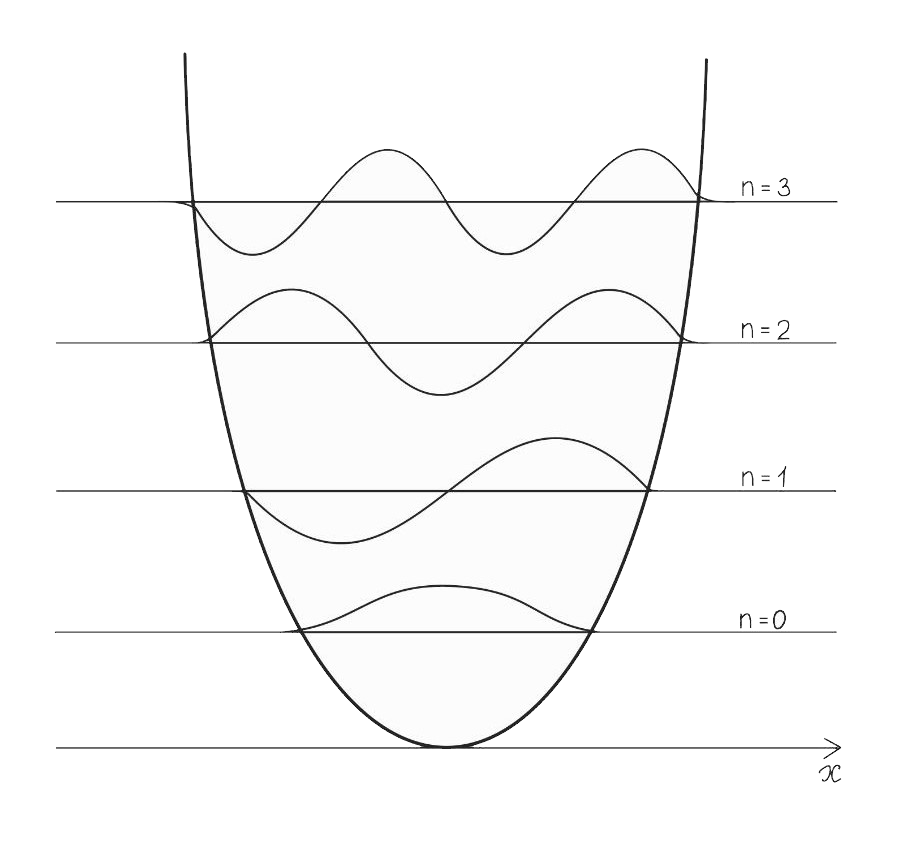
\includegraphics[scale=0.4]{class 6/images/oscillator.png}
\caption{Первые несколько уровней квантового гармонического осциллятора.}
\label{fig 6.8}
\end{figure}
\newpage
Может возникнуть вопрос: чему равны собственные состояния для оператора $\hat{a}$ или $\hat{a}^{\dagger}$ (напомню, что состояния $\ket{n}$ собственные для оператора $\hat{a}^{\dagger}\hat{a}$)? Оказывается, что такие состояния называются когерентными. Они играют большую роль в описании физических систем, так как в когерентном состоянии неопределенность минимальная – значит оно максимально приближает классический осциллятор. Мы не будем обсуждать когерентные состояния подробнее, так как они не присутствует в задачах, однако настоятельно рекомендую прочитать про эту тему самостоятельно. Мы переходим к решению задач на осциллятор.


\excersize{Упражнение №21}{darklavender}
\begin{center}
    \textit{Воспользовавшись повышающим и понижающим операторами $\hat a^+$ и $\hat a$, найдите средние значения оператора $\hat x^2,\,
    \hat x^4$ и $\hat x^{2k+1}$ в $n$-м стационарном состоянии линейного гармонического осциллятора.}
\end{center}
Давайте вспомним из теории, как выглядит оператор координаты $\hat X$: 
\[
\hat x = \frac{x_0}{\sqrt{2}}(\hat a^{\dagger} + \hat a),\quad x_0 = \sqrt{\frac{\hbar}{m\omega}}
\]
Тогда, запишем среднее значение по определению и, используя действия оператора рождения и оператора уничтожения на энергетический уровень n ($\hat a\ket{n} = \sqrt{n}\ket{n-1}$ и $\hat{a}^{\dagger}\ket{n} = \sqrt{n+1}\ket{n+1}$) посчитаем:
\begin{multline*}
    \bra{n}\hat x^2 \ket{n} = \frac{x^2_0}{2}\bra{n}(\hat a^{\dagger} + \hat a)^2\ket{n} = \frac{x^2_0}{2}(\bra{n}\hat a^{\dagger}\hat a^{\dagger}\ket{n} +\bra{n}\hat a\hat a\ket{n} + \bra{n}\hat a^{\dagger}\hat a\ket{n} + \bra{n}\hat a\hat a^{\dagger}\ket{n}) =\\
    \frac{x^2_0}{2}(\sqrt{(n+1)(n+2)}\bra{n}\ket{n+2} + \sqrt{(n)(n-1)}\bra{n}\ket{n-2} + \sqrt{(n+1)(n+1)}\bra{n}\ket{n} + \sqrt{(n) (n)}\bra{n}\ket{n})
\end{multline*}
Мы знаем, что вектора различных уровней ортогональны, а значит все скалярные произведения для различных n будут равны 0. Тогда останется следующее:
\[
\bra{n}\hat x^2\ket{n} = \frac{x^2_0}{2}((n+1) + n) = x^2_0(n + \frac{1}{2})
\]
Поступая точно так же с четвертой степенью, получим:
\[
\bra{n}\hat x^4\ket{n} = \frac{x_0^4}{4}(6n^2 + 6n + 3)
\]
Теперь с нечетной степенью. Достаточно заметить, что в случае разложения по нечетным степеням, у нас не будет членов с последовательными действиями операторов с одинаковыми степенями ($\hat a\hat a^{\dagger},\; \hat a\hat a^{\dagger}\hat a\hat a^{\dagger}$ и т.п.). Тогда все скалярные произведения будут равны нулю. Значит: 
\[
\bra{n}\hat x^{2k+1}\ket{n} = 0
\]
\csquare{darklavender}
\excersize{Упражнение №22}{darklavender}
\begin{center}
    \textit{Частица массы $m$ движется в потенциале трехмерного изотропного осциллятора:}
    \[
    U(r) = \frac{m\omega^2r^2}{2}.
    \]
    \textit{Найдите энергии уровней, кратности их вырождения, а также волновые функции стационарных состояний, разделяя переменные: а) в декартовых координатах, б) в сферических координатах. Обсудите связь задачи с моделью ядерных оболочек и получите первые магические числа: 2, 8, 20.}

    \textit{Определите четности стационарных состояний. Может ли осциллятор, находящийся в состоянии с определенной энергией, обладать отличным от нуля электрическим дипольным моментом (см. задачу 1)?}
\end{center}
В этом семинаре решим только в декартовых координатах. В следующих семинаре, когда пройдём движение в центральном поле, решим в сферических координатах.

Давайте подставим потенциал в уравнение Шрёдингера:
\[
-\frac{\hbar^2}{2m}\Delta\psi(\vec{r}) + \frac{m\omega^2\vec{r}^2}{2}\psi(\vec{r}) = E\psi(\vec{r})
\]
Так как координаты декартовы, можем записать Гамильтониан в виде:
\[
\hat H = \sum\limits_{i=1}^3(-\frac{\hbar^2}{2m}\frac{\partial^2}{\partial x_i^2} + \frac{m\omega^2x_i^2}{2})
\]
Такой гамильтониан коммутирует с каждым из операторов координаты $\hat{x}, \hat{y}, \hat{z}$, а значит решение можно искать в виде произведения их собственных функций. В то же время, это гамильтониан гармонического осциллятора, т.е. его можно описать через оператор $\hat{a}^{\dagger}\hat{a}$. Тогда эти функции будут ещё и собственные для этого оператора. В итоге можем записать волновые функции в следующем виде:
\[
\psi_{n_1n_2n_3}(\vec{r}) = u_{n1}(X)u_{n2}(Y)u_{n3}(Z)
\]
\[
u_{n_i}(X_i) = \frac{1}{\pi^{\frac{1}{4}}\sqrt{2^{n_i}n_i!}}e^{-X^2/2}H_{n_i}(X)
\]
где $H_{n}(X)$ - полиномы Эрмита. Энергия тогда будет иметь вид:
\[
E_n = \hbar\omega(n+\frac{3}{2}), \text{ где } n = n_1 + n_2 + n_3
\]
Давайте посчитаем кратность вырождения уровней. Если мы произвольно задаём $n_1 \leq n$, то тогда для $n_2$ останется $n-n_1+1$ вариантов ($n_2 = 0, 1, ... ,n - n1$). В этом случае $n_3 = n - n_1 - n_2$ зафиксировано, и можно посчитать кратность вырождения, используя формулу арифметической прогрессии: 
\[
\sum\limits_{n_1 = 0}^n n_2 = \sum\limits_{n_1 = 0}^n n-n_1 + 1 = \frac{1}{2}(n+1)(n+2)
\]
Посмотри, что получилось. Если n = 0, то кратность вырождения 1, то есть в стационарном состоянии у нас нет вырождения по координате. Если n = 1, то кратность вырождения 3, то есть на втором уровне у нас три возможных состояний координаты с одинаковым состоянием энергии. Если проследить последовательность, то можно заметить, что это очень сильно напоминает расположение электронов на оболочке атома (без учёта вырождения по спину). И это не просто так! Далее мы увидим, что осциллятором вполне можно приблизить модель атомной оболочки.
\csquare{darklavender}

В следующем семинаре мы обсудим движение в центральном поле и спин.


    \newpage
    \begin{center}
    \section{Семинар VII}
\end{center}
\subsection{Трёхмерное пространство.}
Всё хорошее когда-нибудь заканчивается и настаёт пора суровой реальной жизни. Так и для нас самое время переходить к трехмерному пространству. Давайте попробуем разобраться, как изменится подход к описанию систем такого типа.

Так как пространство трёхмерное, мы рассматриваем трёхмерные операторы $\hat{\Vec{r}} = (\hat{x}, \hat{y}, \hat{z})$ и $\hat{\Vec{p}} = (\hat{p}_x, \hat{p}_y, \hat{p}_z)$. Гамильтониан частицы в поле принимает вид:
\[
\hat{H} = \frac{\hat{p}^2_x}{2M} + \frac{\hat{p}^2_y}{2M} + \frac{\hat{p}^2_z}{2M} + V(\Vec{r})
\]
Тогда стационарное уравнение Шрёдингера принимает вид:
\[
\left[\frac{\hat{p}^2}{2M} + V(\Vec{r})\right]\psi(\Vec{r}) = E\psi(\Vec{r})
\]
или, если расписать оператор импульса в координатном представлении:
\[
\left[-\frac{\hbar^2}{2M}\nabla^2 + V(\Vec{r})\right]\psi(\Vec{r}) = E\psi(\Vec{r})
\]
Теперь мы работаем с трёхмерным дифференциальным уравнением в частных производных. Решение этого уравнения в общем виде весьма затруднительно. Поэтому разберём особо важный для физических задач частный случай, а именно -- \textit{центрально -- симметричный потенциал}. В центрально -- симметричном потенциале имеет вид $V(\Vec{r}) = V(r)$, где $r = \sqrt{x^2 + y^2 + z^2}$. Как потом окажется, в этом случае решать трёхмерное уравнение Шрёдингера гораздо удобнее. Но для начала нужно навести немного математики. Начнём с того, что перейдём к сферической системе координат. Делаем мы это, исходя из опыта работы с классическим случаем. Мы хотим разделить потенциал на три отдельные составляющие -- по одной на каждую переменную. Тогда гильбертово пространство будет состоять из тензорного произведения трёх пространств $\mathbf{V} = \mathbf{V}_r\otimes\mathbf{V}_{\theta}\otimes\mathbf{V}_{\phi}$. 

Осуществим переход к сферическим координатам:
\[
\begin{cases}
x = r \sin \theta \cos \phi,\\
y = r \sin \theta \sin \phi, \\
z = r \cos \theta, \\
\end{cases}
\]
Нам так же понадобится скалярное произведение в сферических координатах. Для этого посчитаем якобиан перехода из декартовой системы в сферическую:
\[
J = \left|\frac{\partial(x, y, z)}{\partial(r, \theta, \phi)}\right| = r^2\sin\theta
\]
Тогда, скалярное произведение запишется в виде:
\[
\bra{\psi}\ket{\phi} = \int\limits_{-\infty}^{+\infty}\int\limits_{-\infty}^{+\infty}\int\limits_{-\infty}^{+\infty}\psi^*(r)\phi(r)dxdydz= \int\limits_0^{2\pi}\int\limits_0^{\pi}\int\limits_0^{\infty}\psi^*(r)\phi(r)r^2\sin\theta dr d\theta d\phi
\]
На практике принято объединять пространства, связанные с угловым движением $\mathbf{Y} = \mathbf{V}_{\theta} + \mathbf{V}_{\phi}$ , и оставлять произведение \textit{радиальной} части и \textit{угловой} $\mathbf{V} = \mathbf{V}_r \otimes \mathbf{Y}$. Элементами этих пространств являются волновые функции радиуса $R(r)$ и волновые функции углов $Y(\theta, \phi)$. Для дальнейшего описания нам понадобится новый оператор -- оператор момента импульса.
\subsection{Оператор момента импульса.}
В соответствии с классическим подходом, введём понятие оператора момента импульса как:
\[
\hat{\Vec{L}} = \hat{\Vec{r}} \times \hat{\Vec{p}}
\]
или, если расписать покомпонентно, получим:
\begin{equation*}
\begin{split}
    \hat{L}_x = \hat{y}\hat{p}_z - \hat{z}\hat{p}_y\\
    \hat{L}_y = \hat{z}\hat{p}_x - \hat{x}\hat{p}_z\\
    \hat{L}_z = \hat{x}\hat{p}_y - \hat{y}\hat{p}_x
\end{split}
\end{equation*}
Давайте найдём все важные коммутаторы и оформим это в виде упражнения:
\excersize{Упражнение №23}{darklavender}
\begin{center}
    \textit{Найдите следующие коммутаторы: $[\hat{L}_j, \hat{r}_k]$, $[\hat{L}_j, \hat{p}_k]$, $[\hat{L}_j, \hat{L}_k]$, $[\hat{L}_j, \hat{r}^2]$, $[\hat{L}_j, \hat{p}^2]$, $[\hat{L}_j, \hat{L}^2]$.}
\end{center}
Для удобства записи вспомним, что такое \textit{символ Леви-Чивита}:
\[
\varepsilon_{ijk} = 
\begin{cases}
    1,\; \text{если чётность перестановки индексов \{i, j, k\} чётная};\\
    -1,\;\text{если чётность перестановки индексов \{i, j, k\} нечётная}; \\
    0,\;\text{иначе}.
\end{cases}
\]
Тогда оператор импульса можно переписать в виде $\hat{L}_j = \varepsilon_{jmn} \hat{r}_m \hat{p}_n$. Используя это обозначение, найдём первый коммутатор:
\begin{multline*}
    [\hat{L}_j, \hat{r}_k] = [\varepsilon_{jmn} \hat{r}_m \hat{p}_n, \hat{r}_k] = \varepsilon_{jmn} \hat{r}_m [\hat{p}_n, \hat{r}_k] = \varepsilon_{jmn}\hat{r}_m(-i\hbar)\delta_{nk} = (\text{сворачиваем } \varepsilon_{jmn}\delta_{nk} = \varepsilon_{jmk} \text{ и,} \\ \text{так как символ Леви-Чивита антисимметричный, заменим } \varepsilon_{jmk} = -\varepsilon_{jkm}) = i\hbar\varepsilon_{jkm}\hat{r}_m.
\end{multline*}
Аналогично с импульсом:
\[
[\hat{L}_j, \hat{p}_k] = [\varepsilon_{jmn} \hat{r}_m \hat{p}_n, \hat{p}_k] = \varepsilon_{jmn} \hat{p}_n [\hat{r}_m, \hat{p}_k] = i\hbar\varepsilon_{jmn}\hat{p}_n\delta_{mk} = i\hbar\varepsilon_{jkn}\hat{p}_n
\]
Сейчас придётся немножко помучиться с индексами, но нам не впервой, так что посчитаем третий коммутатор:
\begin{multline*}
    [\hat{L}_j, \hat{L}_k] = [\varepsilon_{jmn} \hat{r}_m \hat{p}_n, \varepsilon_{klq} \hat{r}_l\hat{p}_q] = \varepsilon_{jmn}\varepsilon_{klq}[\hat{r}_m \hat{p}_n, \hat{r}_l\hat{p}_q] = \varepsilon_{jmn}\varepsilon_{klq}(-i\hbar\delta_{nl}\hat{r}_m\hat{p}_q + i\hbar\delta_{mq}\hat{r}_l\hat{p}_n) = \\
    = -i\hbar\varepsilon_{jml}\varepsilon_{klq}\hat{r}_m\hat{p}_q + i\hbar\varepsilon_{jmn}\varepsilon_{klm}\hat{r}_l\hat{p}_n = -i\hbar\varepsilon_{ljm}\varepsilon_{lqk}\hat{r}_m\hat{p}_q + i\hbar\varepsilon_{mnj}\varepsilon_{mkl}\hat{r}_l\hat{p}_n = \\(\text{разворачиваем произведение символов Леви-Чивиты по формуле } \varepsilon_{ljm}\varepsilon_{lqk} = \delta_{jq}\delta_{mk} - \delta_{jk}\delta_{mq})= \\
    = -i\hbar(\delta_{jq}\delta_{mk} - \delta_{jk}\delta_{mq})\hat{r}_m\hat{p}_q + i\hbar(\delta_{nk}\delta_{jl} - \delta_{nl}\delta_{jk})\hat{r}_l\hat{p}_n = -i\hbar\hat{r}_k\hat{p}_j + i\hbar\delta_{jk}\hat{r}_m\hat{p}_m + i\hbar\hat{r}_j\hat{p}_k - i\hbar\delta_{jk}\hat{r}_l\hat{p}_l \\= -i\hbar\hat{r}_k\hat{p}_j + i\hbar\hat{r}_j\hat{p}_k.
\end{multline*}
Теперь давайте попробуем пойти обратным путём, т.е. выразить полученное выражение через произведение символов Леви-Чивиты. Причём мы хотим подобрать индексы так, чтобы в итоге можно было представить выражение как символ Леви-Чивиты, умноженный на оператор момента импульса.
\[
i\hbar\hat{r}_j\hat{p}_k - i\hbar\hat{r}_k\hat{p}_j = i\hbar(\delta_{jm}\delta_{kn} - \delta_{jn}\delta_{km})\hat{r}_n\hat{p}_m = i\hbar\varepsilon_{ljk}\varepsilon_{lmn}\hat{r}_n\hat{p}_m = i\hbar\varepsilon_{ljk}\hat{L}_q
\]
Приравнивая, получим (тут циклически были переставлены индексы в символе Леви-Чивита для красоты записи):
\[
[\hat{L}_j, \hat{L}_k] = i\hbar\varepsilon_{jkl}\hat{L}_l
\]
Полпути пройдено, осталось посчитать коммутатор с квадратами операторов. Приступим:
\[
[\hat{L}_j, \hat{r}^2] = [\hat{L}_j, \hat{r}_k\hat{r}_k] = 2i\hbar\varepsilon_{jkl}\hat{r}_k\hat{r}_l
\]
Индексы k и l -- немые, значит мы можем менять их как хотим. Давайте поменяем их местами. С одной стороны, это нечётная перестановка, значит $\varepsilon_{jkl} = -\varepsilon_{jlk}$. С другой стороны, операторы координаты коммутируют, а значит $2i\hbar\varepsilon_{jkl}\hat{r}_k\hat{r}_l = 2i\hbar\varepsilon_{jlk}\hat{r}_k\hat{r}_l$. Получается, что единственный вариант, когда это выполняется -- когда это выражение равно нулю.
\[
[\hat{L}_j, \hat{r}^2] = [\hat{L}_j, \hat{r}_k\hat{r}_k] = 0
\]
С импульсом аналогично:
\[
[\hat{L}_j, \hat{p}^2] = 2i\hbar\varepsilon_{jkl}\hat{p}_k\hat{p}_l = 0
\]
Вы удивитесь, но то же самое работает и для момента импульса:
\[
[\hat{L}_j, \hat{L}^2] = 2i\hbar\varepsilon_{jkl}\hat{L}_k\hat{L}_l = 0
\]
Последнее выражение играет важную роль, так как это значит, что в системе могут быть одновременно определены и компонента момента импульса, и его квадрат.
\csquare{darklavender}

Может возникнуть вопрос: для чего мы искали коммутатор с квадратом импульса и координаты? Оказывается, что из факта коммутации оператора момента импульса с ними, мы можем получить, что в случае центрально-симметричного потенциала гамильтониан коммутирует с каждой из компонент и квадратом момента импульса. Действительно, гамильтониан равен: 
\[
\hat{H} = \frac{\hat{p}^2}{2M} + V(\sqrt{\hat{r}^2}).
\]
Коммутация с квадратами как раз показывает, что $[\hat{H}, \hat{L}_i] = 0$ и $[\hat{H}, \hat{L}^2] = 0$. Теперь давайте выразим уравнение Шрёдингера через момент импульса. Для этого нам понадобится связь квадрата момента импульса с операторами импульса и координаты:
\[
\hat{L}^2 = \hat{r}^2\hat{p}^2 - (\hat{\Vec{r}}\hat{\Vec{p}})^2 + i\hbar\hat{\Vec{r}}\hat{\Vec{p}}.
\]
Вывести это можно, честно расписав $\hat{L}^2$ как $\hat{L}_j\hat{L}_k = (\varepsilon_{jlm}\hat{r}_l\hat{p}_m)(\varepsilon_{knq}\hat{r}_n\hat{p}_q)$. Умножив стационарное уравнение Шрёдингера на $\hat{r}^2$ и заменив $\hat{r}^2\hat{p}^2$ на $\hat{L}^2 + (\hat{\Vec{r}}\hat{\Vec{p}})^2 - i\hbar\hat{\Vec{r}}\hat{\Vec{p}}$ , получим:
\[
\left[\frac{(\hat{\Vec{r}}\hat{\Vec{p}})^2 - i\hbar\hat{\Vec{r}}\hat{\Vec{p}}}{2M} + \frac{\hat{L}^2}{2M} + \hat{r}^2 V(\Vec{r})\right]\psi(\Vec{r}) = \hat{r}^2 E\psi(\Vec{r})
\]
Можно заметить, что у нас разделились переменные: первое слагаемое влияет только на радиальную часть, второе -- на вращательную, а третье тоже на радиальную, если потенциал вращательно инвариантен, т.е. $V(\Vec{r}) = V(r)$. Но это пока не показано строго, так как мы работаем в сферических координатах, а значит должны перейти к ним.
\excersize{Упражнение №24}{darklavender}
\begin{center}
    \textit{Найдите представление операторов $\hat{L}^2$, $\hat{\Vec{r}}\hat{\Vec{p}}$ и $(\hat{\Vec{r}}\hat{\Vec{p}})^2$ в сферических координатах.}
\end{center}
Расписав компоненту $\hat{L}_j$ в координатном базисе, получим 
\[
\hat{L}_j = -i\hbar\varepsilon_{jkl}r_k\frac{\partial}{\partial r_l}
\]
Далее я подробно буду расписывать случай только для координаты z, для всех остальных вариантов можно проверить выражения по аналогии. Запишем дифференциал в новых координатах:
\[
\frac{\partial }{\partial z} = \frac{\partial}{\partial r}\frac{\partial r}{\partial z} + \frac{\partial}{\partial \theta}\frac{\partial \theta}{\partial z} + \frac{\partial}{\partial \phi}\frac{\partial \phi}{\partial z}
\]
Выразим переменные сферических координат через переменные декартовых:
\begin{equation*}
    \begin{cases}
        x = r\sin\theta\cos\phi\\
        y = r\sin\theta\sin\phi\\
        z = r\cos\theta
    \end{cases}
    =>
    \begin{cases}
        r = \sqrt{x^2 + y^2 + z^2}\\
        \theta = arccos(\frac{z}{r})\\
        \phi = arctg(\frac{y}{x})
    \end{cases}
\end{equation*}
Тогда, честно дифференцируя и выражая результат в сферических координатах, найдём:
\[
\frac{\partial r}{\partial z} = \frac{z}{\sqrt{x^2 + y^2 + z^2}} = \cos\theta.
\]
\[
\frac{\partial \theta}{\partial z} = \frac{-(x^2+y^2)}{\sqrt{\frac{x^2 + y^2}{x^2+y^2+z^2}}(x^2+y^2+z^2)^{3/2}}= -\frac{r^2\sin^2\theta}{\sqrt{\frac{r^2\sin^2\theta}{r^2}}r^3} = -\frac{\sin\theta}{r} 
\]
\[
\frac{\partial \phi}{\partial z} = 0
\]
Выпишу значение производных по оставшимся компонентам, чтобы читатели могли проверить себя:
\[
\frac{\partial r}{\partial x} = \sin\theta\cos\phi; \; \frac{\partial \theta}{\partial x} = \frac{1}{r}\cos\theta\cos\phi; \; \frac{\partial \phi}{\partial x} = -\frac{1}{r}\frac{\sin\phi}{\sin\theta}.
\]
\[
\frac{\partial r}{\partial y} = \sin\theta\sin\phi; \; \frac{\partial \theta}{\partial y} = \frac{1}{r}\cos\theta\sin\phi; \; \frac{\partial \phi}{\partial y} = \frac{1}{r}\frac{\cos\phi}{\sin\theta}.
\]
Теперь, зная все необходимые частные производные, подставим их в изначальное уравнение и получим:
\[
\frac{\partial }{\partial x} = \sin\theta\cos\phi\frac{\partial}{\partial r} + \frac{1}{r}\cos\theta\cos\phi\frac{\partial}{\partial \theta} -\frac{1}{r}\frac{\sin\phi}{\sin\theta}\frac{\partial}{\partial\phi}
\]
\[
\frac{\partial }{\partial y} = \sin\theta\sin\phi\frac{\partial}{\partial r} + \frac{1}{r}\cos\theta\sin\phi\frac{\partial}{\partial \theta} +\frac{1}{r}\frac{\cos\phi}{\sin\theta}\frac{\partial}{\partial\phi}
\]
\[
\frac{\partial }{\partial z} = \cos\theta\frac{\partial}{\partial r} -\frac{\sin\theta}{r}\frac{\partial}{\partial \theta}
\]
Подставим эти значения в компоненты момента импульса:
\begin{multline*}
\hat{L}_z = -i\hbar(x\frac{\partial}{\partial y} - y\frac{\partial}{\partial x}) = -i\hbar\left(r\sin\theta\cos\phi\left(\sin\theta\sin\phi\frac{\partial}{\partial r} + \frac{1}{r}\cos\theta\sin\phi\frac{\partial}{\partial \theta} +\frac{1}{r}\frac{\cos\phi}{\sin\theta}\frac{\partial}{\partial\phi}\right) - ...\right) = \\
= \left(r\sin^2\theta \cos\phi \sin\phi \frac{\partial}{\partial r} - r\sin^2\theta\cos\phi\sin\phi\frac{\partial}{\partial r} = 0. \text{ Аналогично, второй член сократится}\right) =\\ = -i\hbar\left(r\sin\theta\cos\phi\frac{1}{r}\frac{\cos\phi}{\sin\theta}\frac{\partial}{\partial \phi} + r\sin\theta\sin\phi\frac{1}{r}\frac{\sin\phi}{\sin\theta}\frac{\partial}{\partial \phi} \right) = -i\hbar \left(\cos^2\phi+\sin^2\phi\right)\frac{\partial}{\partial \phi} = -i\hbar\frac{\partial}{\partial \phi}
\end{multline*}
Аналогично, для других компонент:
\[
\hat{L}_x = i\hbar\left(\sin\phi\frac{\partial}{\partial \theta} + ctg\,\theta\cos\phi \frac{\partial}{\partial \phi}\right)
\]
\[
\hat{L}_x = i\hbar\left(-\cos\phi\frac{\partial}{\partial \theta} + ctg\,\theta\sin\phi \frac{\partial}{\partial \phi}\right)
\]
Далее найдём квадрат момента импульса, записав его как: $\hat{L}^2 = \hat{L}^2_x + \hat{L}^2_y + \hat{L}^2_z$:
\[
\hat{L}^2 = -\hbar^2\left[\frac{1}{\sin\theta}\frac{\partial}{\partial \theta}\left( \sin\theta\frac{\partial}{\partial \theta} \right) + \frac{1}{\sin^2\theta}\frac{\partial^2}{\partial\phi^2}\right]
\]
Используя производные в сферических координатах, найдём операторы $\hat{\Vec{r}}\hat{\Vec{p}}$ и $(\hat{\Vec{r}}\hat{\Vec{p}})^2$:
\[
\hat{\Vec{r}}\hat{\Vec{p}} = -i\hbar\frac{\partial}{\partial r}
\]
\[
(\hat{\Vec{r}}\hat{\Vec{p}})^2 = -\hbar^2\left( r^2\frac{\partial^2}{\partial r^2} + r\frac{\partial}{\partial r}\right)
\]
\csquare{darklavender}

Посмотрев на получившиеся операторы, сразу можно заметить, что наше предположение о разделении переменных оказалось верным. Действительно, операторы $\hat{\Vec{r}}\hat{\Vec{p}}$ и $(\hat{\Vec{r}}\hat{\Vec{p}})^2$ содержат в себе только радиальную часть, а $\hat{L}^2$ , наоборот, зависит только от углов. Также мы показали, что оператор $\hat{L}^2$ коммутирует с гамильтонианом. Казалось бы, ну и отлично, давайте будем искать решения уравнений Шрёдингера в собственных состояниях квадрата момента импульса. Однако на деле не всё так просто. Проблема в том, что оператор $\hat{L}^2$, как мы выяснили ранее, локален в $\mathbf{Y}$. Это значит, что собственные состояния эквивалентного для него оператора во всём пространстве $\hat{1}\otimes\hat{L}^2$ имеют собственные состояния $\ket{R}\otimes\ket{\lambda}$, где $\ket{\lambda}$ -- собственное состояния оператора $\hat{L}^2$ в $\mathbf{Y}$, а $\ket{R}$ -- произвольное (!) состояние в $\mathbf{V}_r$. Эта произвольность как раз и мешает нам находить решение в таком виде -- сильная вырожденность собственных значений оператора $\hat{1}\otimes\hat{L}^2$ не даёт нам уверенности в том, что случайно выбранное состояние вида $\ket{R}\otimes\ket{\lambda}$ будет собственным для гамильтониана. Получается, из всего многообразия таких состояний нам нужно отобрать те, которые являются собственными для гамильтониана. Для этого подставим найденные в сферических координатах операторы в уравнение Шрёдингера, запишем волновую функцию как $\psi(r, \theta, \phi) = R(r)Y_{\lambda}(\theta, \phi)$ и заменим оператор $\hat{L}^2$ на его собственное значение: 
\[
\left[-\frac{\hbar^2}{2Mr^2}\left( r^2\frac{\partial^2}{\partial r^2} + 2r\frac{\partial}{\partial r} \right)  + \frac{\lambda}{2M} + r^2V(r)\right]R(r)Y_{\lambda}(\theta, \phi) = r^2ER(r)Y_{\lambda}(\theta, \phi).
\]
Тогда, переписывая $r^2\frac{\partial^2}{\partial r^2} + 2r\frac{\partial}{\partial r}$ как $\frac{\partial}{\partial r}\left( r^2 \frac{\partial}{\partial r}\right)$ и сокращая $Y_{\lambda}(\theta, \phi)$, получим так называемое \textit{радиальное уравнение}:
\[
\left[-\frac{\hbar^2}{2Mr^2}\frac{\partial}{\partial r}\left( r^2 \frac{\partial}{\partial r}\right)  + \frac{\lambda}{2Mr^2} + V(r)\right]R(r) = ER(r).
\]
Получается, что, если радиальная часть волновой функции $\psi(r, \theta, \phi) = R(r)Y_{\lambda}(\theta, \phi)$ удовлетворяет радиальному уравнению, то эта волновая функция является собственное для гамильтониана с собственным значением E. Таким образом, мы разделили задачу на две: нахождение собственных значений $\hat{L}^2$ (приведение к диагональному виду) и решения диффура. Первую часть задачу достаточно решить один раз. Этим мы и займёмся в следующем семинаре.
    \newpage 
    \begin{center}
    \section{Семинар VIII}
\end{center}
\subsection{Собственные значения момента импульса.}
Предыдущий семинар мы закончили на радиальном уравнении:
\[
\left[-\frac{\hbar^2}{2Mr^2}\frac{\partial}{\partial r}\left( r^2 \frac{\partial}{\partial r}\right)  + \frac{\lambda}{2Mr^2} + V(r)\right]R(r) = ER(r).
\]

Напомню, что сейчас мы хотим привести оператор $\hat{L}^2$ к диагональному виду. Однако тут возникает проблема: собственные значения $\lambda$ в $\mathbf{Y}$ вырождены. Соответственно, просто найдя $\lambda$ мы не сможем однозначно идентифицировать для неё собственное состояние $\ket{\lambda}$, так как каждому $\lambda$ будет соответствовать линейное подпространство. Для того, чтобы решить проблему, мы добавим к нашей системе оператор, коммутирующий с оператором $\hat{L}^2$. Тогда в каждом вырожденном подпространстве $\lambda$ мы сможем определить ортонормированный собственный базис, так как у коммутирующих операторов общий набор собственных состояний. Оказывается, что очень удачно для такого решения подходит оператор $\hat{L}_z$, собственные значения которого мы обозначим через $\mu$. Тогда задача сводится к поиску $\ket{\lambda\mu}$, т.е. собственных состояний для операторов $\hat{L}^2$ и $\hat{L}_z$.
\begin{equation*}
    \begin{cases}
        \hat{L^2}\ket{\lambda\mu} = \lambda\ket{\lambda\mu}\\
        \hat{L}_z\ket{\lambda\mu} = \mu\ket{\lambda\mu}
    \end{cases}
\end{equation*}

В целом, можно получить волновые функции состояния $\ket{\lambda\mu}$ , честно решив эту систему уравнений. Однако мы пойдём более ``квантовомеханическим'' путём. Подход будет похож на тот, который мы использовали при анализе осциллятора в шестом семинаре. Давайте введём \textit{повышающий и понижающий} операторы следующим образом:
\begin{equation*}
    \begin{split}
        \hat{L}_+ = \hat{L}_x + i\hat{L}_y  \\
        \hat{L}_- = \hat{L}_x - i\hat{L}_y 
    \end{split}
\end{equation*}

Некоторые особенности этих операторов:
\begin{equation*}
    \begin{aligned}
        a)& \hat{L}_+ = \hat{L}^{\dagger}_-  \\
        b)& \left[\hat{L}_z, \, \hat{L}_{\pm}\right] = \pm\hbar \hat{L}_{\pm},\; \left[\hat{L}^2, \, \hat{L}_{\pm}\right] = 0, \; \left[\hat{L}_+, \, \hat{L}_-\right] = 2\hbar \hat{L}_z \\
        c)& \hat{L}^2 = \hat{L}_+\hat{L}_- + \hat{L}^2_z - \hbar\hat{L}_z
    \end{aligned}
\end{equation*}
Используя полученные коммутационные соотношения, покажем, что состояния $\hat{L}_{\pm}\ket{\lambda\mu}$ являются собственными для операторов $\hat{L}^2$ и $\hat{L}_z$ одновременно, с собственным значениями $\lambda$, $\mu \pm \hbar$. Действительно, подействовав оператором $\hat{L}^2$ на состояние $\hat{L}_{\pm}\ket{\lambda\mu}$, получим:
\[
\hat{L}^2\hat{L}_{\pm}\ket{\lambda\mu} = \hat{L}_{\pm}\hat{L}^2\ket{\lambda\mu} = \lambda\hat{L}_{\pm}\ket{\lambda\mu}
\]
Теперь, подействуем оператором $\hat{L}_z$:
\[
\hat{L}_z\hat{L}_{\pm}\ket{\lambda\mu} = (\hat{L}_{\pm}\hat{L}_z \pm \hbar\hat{L}_{\pm})\ket{\lambda\mu} = (\mu\hat{L}_{\pm} \pm \hbar\hat{L}_{\pm})\ket{\lambda\mu} = (\mu \pm \hbar)\hat{L}_{\pm}\ket{\lambda\mu}
\]

Таким образом мы получили то, что хотели. Далее, продолжая похожие рассуждения, как и в случае с операторами рождения и уничтожения, найдём, как действует оператор $\hat{L}_{\pm}$ на состояние $\ket{\lambda\mu}$:
\[
\hat{L}_{\pm}\ket{\lambda\mu} = \sqrt{\lambda - \mu(\mu \pm \hbar)}\ket{\lambda,\mu\pm\hbar}.
\]

В очередной раз операторы оправдывают своё название. Как видите, мы либо повышаем значение $\mu$ на константу $\hbar$, либо понижаем её на то же значение. Но что это за константа? Давайте разбираться.

Для начала заметим, что выполняется неравенство $\lambda \geq \mu^2$. В самом деле, для оператора $\hat{L}^2 - \hat{L}^2_z$ состояние $\ket{\lambda\mu}$ является собственным с собственным значением $\lambda - \mu^2$. Но, в то же время, этот оператор можно переписать как $\hat{L}^2_x + \hat{L}^2_y$ (так как $\hat{L}^2 = \hat{L}^2_x + \hat{L}^2_y + \hat{L}^2_z$). Этот оператор неотрицательный и имеет неотрицательные собственные значения. Значит, $\lambda - \mu^2 \geq 0\; => \; \lambda \geq \mu^2$.

Используя оператор повышения, мы можем поднять состояние $\ket{\lambda,\mu + j\hbar}$, где $j$ - целое неотрицательное число. Но теперь мы знаем, что $(\mu + j\hbar)^2$ не должно быть больше $\lambda$. Тогда, как и в случае с понижающим оператором, нам нужно поставить условие, что, дойдя до определенного $j = j_0$ у нас получится уравнение $\hat{L}_+\ket{\lambda, \mu + j_0\hbar} = 0$. Найдём, при каком $\lambda$ это выполняется:
\begin{multline*}
\hat{L}_{+}\ket{\lambda,\mu + j_0\hbar} = \sqrt{\lambda - (\mu+j_0\hbar)(\mu + (j_0 + 1)\hbar)}\ket{\lambda,\mu +(j_0 + 1)\hbar)} = 0\; => \\ \lambda = [\mu + j_0\hbar][\mu + \hbar(j_0 + 1)]
\end{multline*}

Аналогично, для понижающего оператора должно выполняться $\hat{L}_-\ket{\lambda,\mu - k_0\hbar} = 0$. Тогда $\lambda = [\mu - k_0\hbar][\mu-\hbar(k_0 + 1)]$ и должно выполняться уравнение:
\[
 [\mu + j_0\hbar][\mu + \hbar(j_0 + 1)]=[\mu - k_0\hbar][\mu-\hbar(k_0 + 1)]
\]
Если, для удобства обозначения мы сделаем замену $\mu + j_0\hbar = x$ и $\mu - (k_0 + 1)\hbar = y$, то уравнение примет вид:
\[
x(x+\hbar) = y(y+\hbar)
\]
Если решить это квадратное уравнение относительно y и учесть, что нам подходит только тот корень, который удовлетворяет условию $x > y$, то получим $y = -(x + \hbar)$ или 
\[
\mu - (k_0 + 1)\hbar = -\mu - (j_0 + 1)\hbar\; => \; \mu = \frac{k_0 - j_0}{2}\hbar.
\]

Определим значение $\lambda$, подставив $\mu$ в уравнение, полученное выше:
\[
\lambda = [\mu + j_0\hbar][\mu + \hbar(j_0+1)] = \frac{k_0 + j_0}{2}\left(\frac{k_0 + j_0}{2} + 1\right)\hbar^2
\]

Сейчас мы определим два важных значения, с которыми вы уже не один раз сталкивались ещё со школы. Пусть $l\equiv \frac{k_0 + j_0}{2}$ - будем называть его \textit{орбитальным квантовым числом}. Его значения лежат в множестве $\{n/2,\, n\in \mathbb{Z}_+\}$, то есть являются целочисленными или полуцелыми\footnote[1]{Отмечу, что пока не было доказано, что l - только целочисленное значение, хотя при рассмотрении атомов мы пользовались только целочисленными орбитальными числами. Объяснение этой особенности будет рассмотрено далее.} неотрицательными числами (0, 1/2, 1, ... ).

Запишем собственное значение $\lambda$  через $l$:
\[
\lambda = \hbar^2(l+1)l
\]
То же самое сделаем и с собственным значением $\mu$:
\[
\mu = (l - j_0)\hbar = (-l + k_0)\hbar
\]
Пусть $m \equiv \mu/\hbar$. Мы видим, что значение $m$ зависит от $l$ и определяется в диапазоне от $-l$ до $l$ с шагом единица. Действительно, по условию $m^2 \leq l(l+1)$. Так как $j_0$ и $k_0$ - целочисленные неотрицательные значения, то шаг может происходить только на единицу. Значит, крайние значения для m - это $l$ и $-l$, иначе неравенство нарушается. Число m мы будем называть \textit{магнитным квантовым числом}. С ним вы тоже уже встречались.

Используя новые обозначения, перепишем полученное ранее действие операторов $\hat{L}_{\pm}$:
\[
\hat{L}_{\pm}\ket{lm} = \hbar\sqrt{l(l+1) - m(m \pm 1)}\ket{l, m \pm 1} = \hbar\sqrt{(l \mp m)(l \pm m + 1)}\ket{l,m\pm 1}
\]

Давайте найдём матричные элементы всех наших новых операторов в общем виде, а затем решим упражнение для конкретного орбитального числа. Начнём с самого простого оператора -- $\hat{L}^2$. Напомню, что матричный элемент -- это конструкция вида $\bra{\psi}\hat{A}\ket{\psi'}$. В нашем случае $\bra{lm}\hat{L}^2\ket{l'm'}$. Итак
\[
\bra{lm}\hat{L}^2\ket{l'm'} = \hbar^2l'(l'+1)\bra{lm}\ket{l'm'} = \hbar^2l'(l'+1)\delta_{ll'}\delta_{mm'}
\]
Далее, для оператора $\hat{L}_z$:
\[
\bra{lm}\hat{L}_z\ket{l'm'} = \hbar m'\bra{lm}\ket{l'm'} = \hbar m'\delta_{ll'}\delta_{mm'}
\]
Для повышающего и понижающего мы уже знаем действие на состояние $\ket{lm}$, так что найти матричный элемент не составит проблемы:
\[
    \bra{lm}\hat{L}_{\pm}\ket{l'm'} = \hbar\sqrt{l'(l'+1) - m'(m' \pm 1)}\delta_{ll'}\delta_{m,m'\pm 1}
\]
Операторы $\hat{L}_x$ и $\hat{L}_y$ выражаются через понижающие и повышающие операторы по определению:
\begin{align*}
    \hat{L}_x & = \frac{\hat{L}_+ + \hat{L}_-}{2};\\
    \hat{L}_y & = \frac{\hat{L}_+ - \hat{L}_-}{2i}
\end{align*}
Тогда, подставляя их в такой форме в выражение для матричных элементов, получим:
\[
\bra{lm}\hat{L}_{x}\ket{l'm'} = \frac{\hbar}{2}\left[\sqrt{l'(l'+1) - m'(m' + 1)}\delta_{ll'}\delta_{m,m' + 1} + \sqrt{l'(l'+1) - m'(m' - 1)}\delta_{ll'}\delta_{m,m' - 1}\right]
\]
\[
\bra{lm}\hat{L}_{y}\ket{l'm'} = \frac{\hbar}{2i}\left[\sqrt{l'(l'+1) - m'(m' + 1)}\delta_{ll'}\delta_{m,m' + 1} - \sqrt{l'(l'+1) - m'(m' - 1)}\delta_{ll'}\delta_{m,m' - 1}\right]
\]
Теперь, зная все матричные элементы, выполним следующее упражнение.
\excersize{Упражнение №25}{darklavender}
\begin{center}
    \textit{Постройте матрицы операторов момента импульса $\hat{L}_x$, $\hat{L}_y$, $\hat{L}_z$, а также $\hat{L}^2$, $\hat{L}_+$ и $\hat{L}_-$ для квантовой системы с орбитальным числом $l = 1$. Как выглядят собственные вектора операторов $\hat{L}^2$ и $\hat{L}_z$?}
\end{center}
Всю ``сложную'' часть мы уже проделали, осталось только подставить значение l = 1 в полученные выше формулы:
\[
\hat{L}^2 \simeq  2\hbar^2 \left(\begin{array}{ccc} 1 & 0 & 0 \\ 0 & 1 & 0 \\ 0 & 0 & 1 \end{array} \right); \; \hat{L}_z \simeq  \hbar \left(\begin{array}{ccc} 1 & 0 & 0 \\ 0 & 0 & 0 \\ 0 & 0 & -1 \end{array} \right)
\]
В остальных операторах значения уйдут с главной диагонали, т.к. в дельтах индексы m отличаются на единицу.
\[
\hat{L}_+ \simeq  \sqrt{2}\hbar \left(\begin{array}{ccc} 0 & 1 & 0 \\ 0 & 0 & 1 \\ 0 & 0 & 0 \end{array} \right); \; \hat{L}_- \simeq  \sqrt{2}\hbar \left(\begin{array}{ccc} 0 & 0 & 0 \\ 1 & 0 & 0 \\ 0 & 1 & 0 \end{array} \right)
\]
\[
\hat{L}_x \simeq  \frac{\hbar}{\sqrt{2}} \left(\begin{array}{ccc} 0 & 1 & 0 \\ 1 & 0 & 1 \\ 0 & 1 & 0 \end{array} \right);\; \hat{L}_y \simeq  \frac{i\hbar}{\sqrt{2}} \left(\begin{array}{ccc} 0 & -1 & 0 \\ 1 & 0 & -1 \\ 0 & 1 & 0 \end{array} \right)
\]

Так как матрицы операторов $\hat{L}^2$ и $\hat{L}_z$ диагональны, найти их собственные вектора несложно -- это просто базисные вектора $ \left(\begin{array}{c} 1 \\ 0  \\ 0  \end{array} \right)$, $ \left(\begin{array}{c} 0 \\ 1 \\ 0  \end{array} \right)$ и $ \left(\begin{array}{c} 0 \\ 0  \\ 1  \end{array} \right)$. 
\csquare{darklavender}

\subsection{Собственные состояния момента импульса}
Процесс нахождение собственных функций, к сожалению, не получится свести к определению новых операторов и чисто квантово-механическому подходу. Поэтому рассуждения и поиск волновых функций я вынес в \nameref{appendix:A}. Здесь же я приведу только ответ.

Итак, волновая функция состояния $\ket{lm}$ задаётся сферическими гармониками:
\[
Y^m_l(\theta, \phi) = \mathcal{N}_l\sqrt{\frac{(l+m)!}{(l-m)!}} \frac{1}{\sin^{m}\theta}\,\frac{d^{l-m}}{d(\cos\theta)^{l-m}}\sin^{2l}\theta e^{im\phi},
\]
где $\mathcal{N}_l = (-1)^l \sqrt{\frac{2l+1}{4\pi}}\frac{1}{2^l l!}$ - коэффициент нормировки.

Вычислим явно сферические гармоники для $l=0$ и $l=1$:
\[
Y^0_0(\theta,\phi) = (-1)^0\sqrt{\frac{1}{4\pi}}\sqrt{\frac{0!}{0!}}\sin^0\theta \frac{d^0}{d(\cos\theta)^0} \sin^0 \theta e^{0} = \sqrt{\frac{1}{4\pi}}
\]
\[
Y^1_1(\theta,\phi) = -\sqrt{\frac{3}{8\pi}}\sin\theta e^{i\phi}
\]
\[
Y^0_1(\theta,\phi) = \sqrt{\frac{3}{4\pi}}\cos\theta
\]
\[
Y^{-1}_1(\theta,\phi) = \sqrt{\frac{3}{8\pi}}\sin\theta e^{-i\phi}
\]

Обсудим вопрос, почему l может быть только целым. Действительно, если l может принимать полуцелые значения, значит m также может быть полуцелым. Тогда, множитель $e^{im\phi}$ даст нам ситуацию, в которой $\psi(r, \theta, \phi) = -\psi(r, \theta, \phi + 2\pi)$. А это невозможно, так как мы работаем в координатном базисе. Значит, l в радиально-симметричном поле должна принимать только целые значения.

\subsection*{Спин.}
Чтобы рассказать про спин подробно, нужно уделять этому целую лекцию (а то и две), поэтому здесь мы ограничимся самым необходимым. Если хотите узнать про спин больше, прочитайте \nameref{appendix:B}. Там я постараюсь раскрыть спин с двух сторон: со стороны чистой математики и со стороны физики. Думаю, его должно быть достаточно для более полного понимания, что же такое этот спин и как с ним обращаться.

Очень упрощая, можно сказать, что спин -- это собственный момент импульса частицы. Это не значит, что она крутится -- просто это экспериментальный факт, который был подтвержден в огромном количестве работ. Стоит воспринимать спин как естественную характеристику частицы.

Итак, теперь общее вращение частицы будет задаваться двумя слагаемыми: $\hat{J} = \hat{L} + \hat{S}$, где $\hat{S}$ - спиновый оператор. Его особенность в том, что он коммутирует с операторами координаты и импульса, а значит никак не действует на них.
\[
\left[\hat{S}_j, \, \hat{x}_k\right] = 0,\; \left[\hat{S}_j, \, \hat{p}_k\right] = 0,\; \left[\hat{S}_j, \, \hat{L}_k\right] = 0.
\]
С самим собой оператор $\hat{S}$ коммутирует так же, как и оператор момента импульса.
\[
\left[\hat{S}_j, \, \hat{S}_k\right] = i\hbar\varepsilon_{jkl}\hat{S}_l
\]
Так же, как и у операторов момента импульса, у состояний спина есть повышающие и понижающие операторы.
\[
\hat{S}_{\pm}\ket{s, m_s} = \sqrt{s(s+1) + m_s(m_s \pm 1)}\ket{s, m_s \pm 1}
\]
И точно так же должны выполняться следующие уравнения:
\[
\hat{S}^2\ket{s,m_s} = \hbar^2 s(s+ 1)\ket{s,m_s}, \quad \hat{S}_z\ket{s,m_s} = \hbar m_s\ket{s,m_s}
\]
Аналогично для проекций на другие оси:
\begin{align*}
    \hat{S}_x & = \frac{\hat{S}_+ + \hat{S}_-}{2};\\
    \hat{S}_y & = \frac{\hat{S}_+ - \hat{S}_-}{2i}
\end{align*}
Соответственно, как и в случае момента импульса, у спина будет проекция на ось Z. Обозначаться она будет $m_s$. Ведёт она себя также, как и m - её значения лежат во множестве {-s, -s + 1, ..., s}. Разница в том, что спин может принимать полуцелые значения -- значит, и проекция может быть полуцелая.

Давайте рассмотрим два самых основных примера -- $S = 0$ и $S = 1/2$.
\begin{itemize}
    \item $S = 0$. Тогда и проекция спина на ось z тоже равна нулю: $S_z = 0$. Тогда $\hat{S} = 0$ и волновые функции будут такими, какими мы их знали до того, как появилась внутренняя степень свободы. Примеры частиц с нулевым спином: Бозон Хиггса, $\pi$-мезон.
    \item $S = 1/2$. Проекция спина на ось теперь имеет две компоненты: $S_z = \{1/2, -1/2\}$. Обозначим состояние спина ``вверх'' (в смысле положительной проекции на z) как $\ket{\uparrow} = \ket{1/2,\, 1/2}$, а состояние ``вниз'' -- $\ket{\downarrow} = \ket{1/2, -1/2}$. Посмотрим, как на эти состояния действуют разные операторы.
    \begin{align*}
        &S_z\ket{\uparrow} = \hbar/2\ket{\uparrow}, \quad\, S_z\ket{\downarrow} = -\hbar/2 \ket{\downarrow}\\
        &S_+\ket{\downarrow} = \hbar\ket{\uparrow},\qquad S_+\ket{\uparrow} = 0\\
        &S_-\ket{\uparrow} = -\hbar\ket{\downarrow},\quad\, S_-\ket{\downarrow} = 0\\
        &S_x\ket{\uparrow} =\hbar/2\ket{\downarrow}, \quad\, S_y\ket{\uparrow} =-i\hbar/2\ket{\downarrow}
    \end{align*}
    Зная, как действуют операторы на состояния вверх и вниз, найдём их матрицы:
    \[
    \hat{S}_i \simeq \left(\begin{array}{cc}
        \bra{\uparrow}\hat{S}_i\ket{\uparrow} & \bra{\uparrow}\hat{S}_i\ket{\downarrow} \\
        \bra{\downarrow}\hat{S}_i\ket{\uparrow}  & \bra{\downarrow}\hat{S}_i\ket{\downarrow}
    \end{array}
    \right) = \frac{\hbar}{2}\hat{\sigma}_i,
    \]
    где $\sigma_i$ - \textit{матрицы Паули}. Поговорим про них подробнее, как только найдём, чему они равны. Итак:
    \begin{align*}
    &S_x = \frac{\hbar}{2}\sigma_x = \frac{\hbar}{2}\left(\begin{array}{cc} 0 & 1\\ 1 & 0 \end{array}\right),\\
    &S_y = \frac{\hbar}{2}\sigma_y = \frac{\hbar}{2}\left(\begin{array}{cc} 0 & -i\\ i & 0 \end{array}\right),\\
    &S_z = \frac{\hbar}{2}\sigma_z = \frac{\hbar}{2}\left(\begin{array}{cc} 1 & 0\\ 0 & -1 \end{array}\right).
    \end{align*}
\end{itemize}
Мы видим, что матрицы Паули -- унитарные и эрмитовые матрицы, которыми можно представить обезразмеренный оператор спина. Давайте решим несколько упражнений, чтобы подробнее разобраться с их свойствами.
\excersize{Упражнение №26}{darklavender}
\begin{center}
    \textit{Докажите справедливость следующих соотношений для матриц Паули:}
    \[
    \hat{\sigma}_k\hat{\sigma}_l = \delta_{kl} + ie_{klm}\hat{\sigma_m}
    \]
    \[
    (\hat{\boldsymbol{\sigma}}\mathbf{a})(\hat{\boldsymbol{\sigma}}\mathbf{b}) = (\mathbf{ab}) + i(\boldsymbol{\sigma}[\mathbf{a} \cross \mathbf{b}])
    \]
\end{center}
Ещё раз выпишем явный вид матриц паули для спина $S=1/2$:
\[
    \hat{\sigma}_x = \left(\begin{array}{cc}
        0 & 1 \\
        1 & 0
    \end{array}
    \right), 
    \hat{\sigma}_y = \left(\begin{array}{cc}
        0 & -i \\
        i & 0
    \end{array}
    \right),
    \hat{\sigma}_z = \left(\begin{array}{cc}
        1 & 0 \\
        0 & -1
    \end{array}
    \right)
\]
Данные матрицы обладают следующими свойствами:
\begin{itemize}
    \item $\hat{\sigma}^2 = \hat{1}$,
    \item $[\hat{\sigma}_k, \hat{\sigma}_l] = 2ie_{klm}\sigma_m$,
    \item $\{\hat{\sigma}_k, \hat{\sigma}_l\} = 2\delta_{kl}$, где $\{\hat{\sigma}_k, \hat{\sigma}_l\} = \hat{\sigma}_k\hat{\sigma}_l + \hat{\sigma}_l\hat{\sigma}_k$ -- антикоммутатор.
\end{itemize}
Пользуясь данными свойствами, можем записать:
\[
\hat{\sigma_k}\hat{\sigma_l} = \frac{1}{2}([\hat{\sigma}_k, \hat{\sigma}_l] + \{\hat{\sigma}_k + \hat{\sigma}_l\}) = \frac{1}{2}(2ie_{klm}\sigma_m + 2\delta_{kl}) = \delta_{kl} + ie_{klm}\hat{\sigma}_m,
\]
\[
(\boldsymbol{\sigma}\mathbf{a})(\boldsymbol{\sigma}\mathbf{b}) = \hat{\sigma}_ka_k\hat{\sigma}_lb_l = \hat{\sigma}_k\hat{\sigma}_la_kb_l = (ie_{klm}\hat{\sigma_m} + \delta_{kl})a_kb_l = ie_{klm}\sigma_ma_kb_l + a_kb_k = i(\hat{\sigma}[\mathbf{a}\cross\mathbf{b}]) + (\mathbf{a}\mathbf{b}).
\]
\csquare{darklavender}


\excersize{Упражнение №27}{darklavender}
\begin{center}
    \textit{Найдите собственные значения и собственные векторы спинового оператора $\hat{\sigma}_n = (\hat{\Vec{\sigma}}, \Vec{n})$, где $\Vec{n}$ -- единичный вектор с составляющими:}
    \[
    \Vec{n} = (\sin\theta\cos\phi, \sin\theta\sin\phi, \cos\theta)
    \]
    \textit{Обсудите случаи, когда вектор $\Vec{n}$ направлен вдоль осей $x$, $y$ и $z$.}
\end{center}
Запишем скалярное произведение вектора матриц паули на вектор $\Vec{n}$:
\begin{align*}
    \hat{\sigma}_n & = (\hat{\Vec{\sigma}}, \Vec{n}) = \hat{\sigma}_x n_x + \hat{\sigma}_y n_y + \hat{\sigma}_z n_z = \left(\begin{array}{cc}
        \cos\theta & \sin\theta(\cos\phi - i\sin\phi) \\
        \sin\theta(\cos\phi + i\sin\phi)  & -\cos\Phi
    \end{array}
    \right) = \\ 
    & = 
    \left(\begin{array}{cc}
        \cos\theta & e^{-i\phi} \sin\theta\\
        e^{i\phi} \sin\theta & -\cos\Phi
    \end{array}
    \right)
\end{align*}
Теперь, зная явный вид оператора $\hat{\Vec{\sigma}}_n$, можем решить характеристическое уравнение и найти собственные значения и векторы:

\begin{align*}
    &|\hat{\Vec{\sigma}}_{n} - \lambda E| = \left|\begin{array}{cc}
        \cos\theta - \lambda & e^{-i\phi}\sin\theta \\
         e^{i\phi} & -\cos\theta - \lambda
    \end{array}
    \right| = -\cos^2\theta + \lambda^2 -\sin^2\theta = \lambda^2 - 1 = 0 \; => 
    \\ & => \lambda = \pm 1
\end{align*}
Соответствующие этим собственным значениям собственные функции (нормированные на единицу) имеют вид:
\[
\Psi_1 = \left(\begin{array}{c}
     \cos \frac{\theta}{2} \\
     e^{i\phi} \sin\frac{\theta}{2}
\end{array}
\right),\;
\Psi_{-1} = \left(\begin{array}{c}
    -sin\frac{\theta}{2} \\
    e^{i\phi}\cos\frac{\theta}{2}
\end{array}
\right)
\]
Вектор-функции, элементы которых определяют состояние спина у частиц, мы будем называть \textit{спинорами}. Линейная комбинация функций $\Psi_1$ и $\Psi_2$ как раз и образует спинор. Запомните это обозначение, в будущем оно нам ещё понадобится.
Рассмотрим случаи, когда $\Vec{n}$ направлен вдоль осей $x$, $y$ и $z$:
\begin{enumerate}
    \item $\Vec{n} = (1, 0, 0) \; => \; \theta = \frac{\pi}{2}, \; \phi = 0.$ Подставляя данные значения в найденные собственные функции, получим $\Psi_1 = \left(\begin{array}{c} \frac{\sqrt{2}}{2} \\ \frac{\sqrt{2}}{2} \end{array} \right),\;
    \Psi_{-1} = \left(\begin{array}{c} -\frac{\sqrt{2}}{2} \\ \frac{\sqrt{2}}{2}\end{array}\right)$
    \item $\Vec{n} = (0, 1, 0) \; => \; \theta = \phi = \frac{\pi}{2}$, откуда $\Psi_1 = \left(\begin{array}{c} \frac{\sqrt{2}}{2} \\ \frac{i\sqrt{2}}{2} \end{array}\right),\;
    \Psi_{-1} = \left(\begin{array}{c} -\frac{\sqrt{2}}{2} \\ \frac{i\sqrt{2}}{2} \end{array}\right)$
    \item $\Vec{n} = (0, 0, 1) \; => \; \theta = 0, \; \phi$ любой, откуда $\Psi_1 = \left(\begin{array}{c} 1 \\ 0 \end{array} \right),\;
    \Psi_{-1} = \left(\begin{array}{c} 0 \\ 1 \end{array}\right)$ 
\end{enumerate}
Последний результат особенно важен, так как с помощью него мы будем обозначать волновые функции введённых выше состояний вверх $\ket{\uparrow}$ и вниз $\ket{\downarrow}$.
\csquare{darklavender}
Теперь, когда мы разобрались с матрицами Паули, можно порешать упражнения про спин.
\excersize{Упражнение №28}{darklavender}
\begin{center}
    \textit{Пусть электрон находится в состоянии с проекцией спина на ось $z$, равной $1/2$. Найдите вероятность того, что проекция спина этого электрона на направление $n$ равна $1/2$ (или $-1/2$).}
\end{center}
Из прошлого упражнения мы знаем, как выглядит волновая функция для спина вверх: $\psi_{1/2} = \left(\begin{array}{c} 1 \\ 0 \end{array}\right)$. Так же мы знаем базисные вектора для электрона, спин которого равен 1/2: $\Psi_1 = \left(\begin{array}{c}  \cos \frac{\theta}{2} \\ e^{i\phi} \sin\frac{\theta}{2}\end{array}\right),\; \Psi_{-1} = \left(\begin{array}{c} -sin\frac{\theta}{2} \\ e^{i\phi}\cos\frac{\theta}{2} \end{array} \right)$. Разложим исходное состояние $\psi_{1/2}$ по этим базисным векторам:
\[
\psi_{1/2} = (\Psi_1^{\dagger}\psi_{1/2})\Psi_1 + (\Psi_{-1}^{\dagger}\psi_{1/2})\Psi_{-1}
\]
Заметим, что $\Psi_1^{+} = (\cos\frac{\theta}{2}, e^{-i\phi}\sin\frac{\theta}{2}), \; \Psi_{-1}^{+} = (-\sin\frac{\theta}{2}, e^{i\phi}\cos\frac{\theta}{2})$, откуда
\begin{align*}
    \psi_{1/2} &= (\cos\frac{\theta}{2}, e^{-i\phi}\sin\frac{\theta}{2}) \left(\begin{array}{c} 1 \\ 0 \end{array}\right)\Psi_1 + (-\sin\frac{\theta}{2}, e^{i\phi}\cos\frac{\theta}{2}) \left(\begin{array}{c}
    1 \\ 0 \end{array}\right)\Psi_{-1} = \\
\\ &= \cos\frac{\theta}{2}\Psi_1 - \sin\frac{\theta}{2}\Psi_{-1}
\end{align*}
Как мы помним, если у нас есть разложение нашего состояния, то его вероятность оказаться в каком-то из состояний есть модуль квадрата коэффициента, стоящего при этом состоянии. Тогда, запишем итоговые вероятности:
\[
    P(S_z = 1/2) = \cos^2\frac{\theta}{2},\quad P(S_z = -1/2) = \sin^2\frac{\theta}{2},
\]
\csquare{darklavender}
    \newpage
    \begin{center}
    \section{Семинар IX}
\end{center}
\subsection{Атом водорода.}
Давайте применим полученные нами знания на практике. Попробуем решить радиальное уравнение для атома водорода. В атоме водорода электро движется в электростатическом потенциале, создаваемом тяжелым ядром. Потенциал имеет следующий вид:
\[
V(r) = \frac{e^2}{r}, \text{где e - заряд электрона}.
\]
Видим, что потенциал зависит только от r - значит, задача об атоме водорода представляет собой частный случай движения в центральном поле. Из предыдущих семинаров мы знаем как выглядит волновая функция этой частицы:
\[
\Psi_{nlm}(r, \theta, \phi) = R_{nl}(r)Y^m_l(\theta, \phi).
\]
Что значит первый индекс n - выясним в этом семинаре. Угловая часть нам известна, осталось найти только радиальную часть. Значит, надо решить радиальное уравнение:
\[
\left[ -\frac{\hbar^2}{2Mr^2}\frac{\partial}{\partial r}(r^2 \frac{\partial}{\partial r}) + \frac{\hbar^2 l(l+1)}{2Mr^2} - \frac{e^2}{r}\right]R_{nl}(r) = ER_{nl}(r)
\]
Сделаем замену переменной $R_{nl}=U_{nl}(r)/r$ и перепишем уравнение через новую переменную:
\[
\frac{1}{r^2}\frac{\partial}{\partial r}\left[ r^2 \frac{\partial}{\partial r} R_{nl} \right] = \frac{1}{r^2}\frac{\partial}{\partial r}\left[ r^2 \frac{\partial}{\partial r} \frac{U_{nl}}{r} \right] = \frac{1}{r^2}\frac{\partial}{\partial r}\left[ r^2 (\frac{U'_{nl}}{r} - \frac{U_{nl}}{r^2}) \right] =  \frac{1}{r^2}\left(rU''_{nl}\right) = \frac{U''_{nl}}{r} =>
\]
\[
=>  \left[ -\frac{\hbar^2}{2M}\frac{\partial^2}{\partial r^2} + \frac{\hbar^2 l(l+1)}{2Mr^2} - \frac{e^2}{r}\right]U_{nl}(r) = EU_{nl}(r)
\]
Давайте рассмотрим асимптотики данного уравнения при $r \rightarrow 0$ и $r \rightarrow +\infty$. При $r \rightarrow 0$ доминируют члены с минимальными степенями (максимальными в знаменателе), то есть первый и второй член в квадратных скобках. Перепишем уравнение, оставив только их:
\[
\frac{\partial^2}{\partial r^2} U_{nl}(r) = \frac{l(l+1)}{r^2} U_{nl}(r)
\]
Это уравнение Коши-Эйлера (решается заменой $U_{nl} = r^m$), его решением будет
\[
U_{nl}(r) = c_1r^{l+1} + c_2 r^{-l}
\]
Второе слагаемое отпадает, чтобы волновая функция не имела разрыва при r = 0.

Представим нашу функцию в виде ряда 
\[
U_{nl} = \sum\limits_{j=l+1}^{n}A_j r^j e^{-\kappa r},
\]
где n - некоторое натуральное число и $A_{j+1} \neq 0$ - действительные коэффициенты. Найдём коэффициент $\kappa$, рассмотрев этот ряд и радиальное уравнение при $r \rightarrow +\infty$. В это случае доминировать будут члены с максимальной степенью, т.е. правая часть уравнения. Найдём производную ряда:
\[
\frac{\partial^2}{\partial r^2} U_{nl}(r) =  \sum\limits_{j=l+1}^{n} A_j[\kappa^2r^j - 2\kappa jr^{j-1} + j(j-1)r^{j-2}]e^{-\kappa r}.
\]
Тогда, подставляя максимальную степень, получим:
\[
 -\frac{\hbar^2}{2M}A_n\kappa^2r^n e^{-\kappa r} = EA_n r^n e^{-\kappa r}
\]
Отсюда $\kappa = \sqrt{-2ME}/\hbar$.

Теперь найдём коэффициенты $A_j$ и $n$. Для этого подставим в радиальное уравнение функцию $U_{nl}(r)$ в виде ряда, умножим обе стороны на $2M/\hbar^2$ и выразим энергию через $E = -\hbar^2\kappa^2/2M$. Тогда уравнение преобразуется к следующему виду:
\begin{align*}
    &2\kappa\sum\limits_{j = l+1}^n jA_j r^{j-1} - \sum\limits_{j = l+1}^n j(j-1)A_j r^{j-2} + l(l+1)\sum\limits_{j = l+1}^n A_j r^{j-2} - \\
    & - \frac{2Me^2}{\hbar^2}\sum\limits_{j = l+1}^n jA_j r^{j-1} =0
\end{align*}
Сгруппируем подобные члены и перепишем выражение:
\[
\sum\limits_{j = l+1}^n\left(2\kappa j - \frac{2Me^2}{\hbar^2}\right)A_j r^{j-1} + \sum\limits_{j = l+1}^n [l(l+1) - j(j-1)] A_j r^{j-2} =0
\]
Если во второй сумме сделать замену на $j' = j + 1$, можно заметить, что при $j'=l$ выражение внутри суммы равно нулю. Значит, суммирование мы можем начать с $j'= l+ 1$. Тогда можно переписать:
\[
\sum\limits_{j = l+1}^n\left[\left(2\kappa j - \frac{2Me^2}{\hbar^2}\right)A_j+ [l(l+1) - j(j+1)] A_{j+1} \right]r^{j-1} = 0
\]
Этот многочлен равен нулю при любой степени r тогда, когда выполняется рекурсивное соотношение
\[
\left(2\kappa j - \frac{2}{a}\right)A_j+ [l(l+1) - j(j+1)] A_{j+1} = 0
\]
Здесь мы ввели новую важную величину $a = \frac{\hbar^2}{Me^2} \sim 0.53 \text{\r{A}}$ - \textit{боровский радиус}. Его физический смысл будет понятен чуть позже.

С коэффициентами A разобрались, осталось найти условие на n. Можно появиться вопрос: почему мы вообще решили, что сумма должна быть конечна? Оказывается, что получившийся ряд расходится, если $n=\infty$. Действительно, при больших j $A_j \sim (2\kappa)^j/j!$, и тогда функция имеет вид
\[
U_{nl} \sim \sum\limits_j\frac{(2\kappa r)^j}{j!}e^{-\kappa r} \rightarrow e^{2\kappa r}e^{-\kappa r} = e^{\kappa r}
\]
Волновая функция, которая стремится к бесконечности, нефизична. Значит, n должно быть меньше бесконечности. Условие того, что сумма конечна, выполняется, если множитель перед $A_j$ обнуляется при некотором $j = n$. В этом случае
\[
2\kappa n = \frac{2}{a}
\]
и все $A_j$ при $j > n$ обнуляются.

Теперь мы обладаем достаточным количеством знаний, чтобы найти радиальные волновые функции для конкретных значений $n$ и $l$. Попробуем это сделать в виде упражнения.
\newpage
\excersize{Упражнение №29}{darklavender}
\begin{center}
    \textit{Вычислите радиальные волновые функции $R_{nl}(r)$ атома водорода при $ a)\;n = 1,\, l =0$, $b)\;n = 2,\, l =0$ и $c)\;n = 2,\, l =1$}
\end{center}
a)  При $n = 1,\, l=0$ получим равенство $\kappa = 1/a$. Из всех коэффициентов $A_j$ ненулевым остаётся только $A_1$, так как значения $j$ лежат в промежутке от $l+1$ до $n$. Тогда, вспоминая, что $R_{nl}(r) = U_{nl}(r)/r$, получаем
\[
R_{10}(r) = A_1e^{-r/a}
\]
Получим значение коэффициента $A_1$ из нормировки волновой функции:
\[
\int\limits_0^{+\infty}|R_{10}(r)|^2 r^2 dr = A^2_1\int\limits_0^{+\infty}e^{-2r/a}r^2 dr = A^2_1 2!(\frac{a}{2})^3 = \frac{a^3}{4}A^2_1 = 1\;=>
\]
\[
=>\; A_1 = 2a^{-3/2}.
\]
Тогда итоговая радиальная часть волновой функции имеет вид
\[
R_{10}(r) = 2a^{-3/2}e^{-r/a}
\]
b) При $n = 2,\, l=0$ получим $\kappa = 1/2a$. В этот раз не будут обнуляться у нас два коэффициента - $A_1$ и $A_2$. В нашем случае они связаны соотношением
\[
\left[ 2\kappa - \frac{2}{a} \right]A_1 - 2A_2 = 0\; =>\; A_2 = -\frac{A_1}{2a}
\]
Тогда радиальная часть волновой функции имеет вид
\[
R_{20}(r) = A_1\left( 1 - \frac{r}{2a} \right) e^{-r/2a}
\]
Отнормируем:
\[
\int\limits_0^{+\infty}|R_{20}(r)|^2 r^2 dr = A^2_1\int\limits_0^{+\infty}\left( r^2 - \frac{r^3}{a} +\frac{r^4}{4a^2} \right)e^{-r/a} dr = A^2_1 a^3 (2! - 3! + 4!/4) = 2A^2_1 a^3 = 1\;=>
\]
\[
=>\; A_1 = (2a^3)^{-1/2}.
\]
Итоговый вид:
\[
R_{20}(r) = (2a^3)^{-1/2}\left( 1 - \frac{r}{2a} \right) e^{-r/2a}
\]
c) Для последнего случая $n=2,\, l=1$ у нас остаётся только коэффициент $A_2$, радиальная волновая функция равна
\[
R_{21}(r) = A_2re^{-r/2a}
\]
Нормируя, получим
\[
\int\limits_0^{+\infty}|R_{21}(r)|^2 r^2 dr = A^2_2\int\limits_0^{+\infty}r^4 e^{-r/a} dr = 4! A^2_2 a^5 = 1\;=>
\]
\[
=>\; A_2 = (24a^5)^{-1/2}.
\]

Итог:

\[
R_{21}(r) = (24a^5)^{-1/2}re^{-r/2a}
\]
\csquare{darklavender}

Из этого упражнения становится чуть понятнее, в чём физический смысл боровского радиуса: он определяет характерный размер волновых функций, а также примерный радиус орбитали основного состояния.

Теперь определим энергетический спектр атома водорода. У нас для этого уже всё готово -- достаточно соединить два уравнения на $\kappa$ (выраженное через n и через E):
\[
E_n = -\frac{1}{2M}\left(\frac{\hbar}{na}\right)^2 = -\frac{M}{2}\left(\frac{e^2}{n\hbar}\right)^2
\]
Заметим, что энергия от $l$ не зависит, только от n. Поэтому n называется \textit{главным квантовым числом}. Оно определяет степень вырождения по остальным квантовым числам. Давайте вспомним все квантовые числа, которые у нас имеются на данный момент:
\begin{itemize}
    \item $n \in \mathbb{N}$ - главное квантовое число
    \item $l \in {0, 1, 2, ..., n-1}$ - орбитальное квантовое число
    \item $m \in {-l, -l+1, ... , l-1, l}$ - магнитное квантовое число.
\end{itemize}
Получается, что при заданном главном квантовом числе $n$, вырождение определяется как $2n^2$. Действительно, количество значений $l$ равно n, степень вырождения $l$ в свою очередь $2l+1$. Тогда, посчитав сумму первых n членов арифметической прогрессии, получим $\sum\limits_{l=0}^{n-1}(2l +1 ) = n^2$. Двойка появится, если мы учтём вырождение по спину: он может принимать два значения - $\pm 1/2$.

\subsection{Решение задач в трехмерном пространстве.}
Посчитаем средние значения трёх координат для атома водорода:
\excersize{Упражнение №30}{darklavender}
\begin{center}
    \textit{Атом водорода находится в состоянии с главным квантовым числом $n = 2$. Вычислите все возможные проекции дипольного момента атома $\mathbf{d} = \bra{\psi}e\hat{r}_j\ket{\psi'}$}
\end{center}
Дипольный момент характеризует переход атома из одного состояния в другое после излучения фотона Отсюда становится понятно, что остаться на одном и том же уровне электрон никак не может - если фотон излучился, то энергия должна уменьшится. Давайте покажем это на одной из проекций. Напомню, что $r_j = r\sin\theta\cos\phi$, $r\sin\theta\sin\phi$, $r\cos\theta$ для $x$, $y$ и $z$ соответственно.
\begin{align*}
    \bra{2,\, 0,\, 0}z\ket{2,\, 0,\, 0} &= \int\limits_{0}^{+\infty}\int\limits_{0}^{\pi}\int\limits_{0}^{2\pi}(R_{20})^2(Y^0_0)^2r\cos\theta \, r^2\sin\theta dr\, d\theta\, d\phi =\\& = \frac{1}{8a^3\pi} \int\limits_{0}^{+\infty}\int\limits_{0}^{\pi}\int\limits_{0}^{2\pi} \left( 1 - \frac{r}{2a} \right)^2 e^{-r/a} r^3\cos\theta\sin\theta\, dr \, d\theta\, d\phi = \\ & = \left(\int\limits_{0}^{\pi} \cos\theta \sin\theta d\theta = 0\right) = 0
\end{align*}
То же самое будет и со всеми остальными проекциями. Теперь посмотрим на переходы между энергетическими уровнями. Давайте попробуем сделать это в общем виде:
\begin{align*}
    \bra{nlm}\begin{pmatrix} x \\ y \\ z \end{pmatrix}\ket{n'l'm'} &= \int\limits_{0}^{+\infty} r^2 R^*_{nl} R_{n'l'} dr \int\limits_{0}^{\pi}\sin\theta\,d\theta\int\limits_{0}^{2\pi}(Y^{m'}_{l'}) (Y^m_l)^*d\phi \begin{pmatrix} r\sin\theta\cos\phi \\ r\sin\theta\sin\phi \\ r\cos\theta \end{pmatrix}\\ & = I_r(n,\,l,\,n',\,l')I_{\theta\phi}(l,\,m,\,l',\,m'),
\end{align*}
где $I_r(n,\,l,\,n',\,l')$ и $I_{\theta\phi}(l,\,m,\,l',\,m')$ - радиальный и угловой интеграл, соответственно:
\[
I_r(n,\,l,\,n',\,l') = \int\limits_{0}^{+\infty} r^3 R^*_{nl} R_{n'l'} dr
\]
\[
I_{\theta\phi}(l,\,m,\,l',\,m') = \int\limits_{0}^{\pi}\sin\theta\,d\theta\int\limits_{0}^{2\pi}(Y^{n'}_{l'}) (Y^n_l)^*d\phi \begin{pmatrix} \sin\theta\cos\phi \\ \sin\theta\sin\phi \\ \cos\theta \end{pmatrix}
\]

Посчитаем сначала радиальные интегралы, так как их всего два.
\begin{align*}
    I_r(1,\,0,\,2,\,0) = \int\limits_{0}^{+\infty} R_{10}^*\,R_{20}\,r^3\,dr &= \int\limits_{0}^{+\infty} 2a^{-\frac{3}{2}} e^{-\frac{r}{a}} \, (2a)^{-\frac{1}{2}} (1 - \frac{r}{2a}) e^{-\frac{r}{2a}} \, r^3 dr = \\& = \frac{\sqrt{2}}{a^3} \int\limits_{0}^{+\infty} e^{-\frac{3}{2a}r} r^3 dr - \frac{1}{\sqrt{2}a^4} \int\limits_{0}^{+\infty} e^{-\frac{3}{2a}} r^4 dr = \\& = \left(\int\limits_{0}^{+\infty} x^n e^{-ax} dx = \frac{n!}{a^{n + 1}}, n = 0, 1, 2..., a > 0\right) = -\frac{32\sqrt{2}}{81} a \\
\end{align*}
\begin{align*}
    I_r(1, 0, 2, 1) = \int\limits_{0}^{+\infty} R_{10}^* R_{21} r^3 dr &= \int\limits_{0}^{+\infty} 2a^{-\frac{3}{2}} e^{-\frac{r}{a}} * (24a^5)^{-\frac{1}{2}} r e^{-\frac{r}{2a}} * r^3 dr = \frac{256}{81} \frac{a}{\sqrt{6}} 
\end{align*}
Теперь посчитаем угловые интегралы. Начнём с того, что убедимся, что переход между уровнем $\bra{1,\,0,\,0}\mathbf{r}\ket{2,\,0,\,0}$ невозможен.
\begin{align*}
    I_{\theta\phi}(0,\,0,\,0,\,0) &= \int\limits_{0}^{\pi}\sin\theta\,d\theta\int\limits_{0}^{2\pi}(Y^0_0)^2d\phi \begin{pmatrix} \sin\theta\cos\phi \\ \sin\theta\sin\phi \\ \cos\theta \end{pmatrix} = \\& = \int\limits_{0}^{\pi} \begin{pmatrix} \sin^2 \theta \\ \sin^2 \theta \\ \sin\theta\cos\theta \end{pmatrix} \, d\theta \int\limits_{0}^{2\pi} \left(\frac{1}{2\sqrt{\pi}}\right)^2 \begin{pmatrix} \cos\phi \\ \sin\phi \\ 1 \end{pmatrix} \, d\phi = \\& = \left( \int\limits_{0}^{2\pi} \cos\phi d\phi = \int\limits_{0}^{2\pi} \sin\phi d\phi = \int\limits_{0}^{\pi} \sin\theta \cos\theta d\theta = 0 \right) = \begin{pmatrix} 0 \\ 0 \\ 0
    \end{pmatrix}
\end{align*}
Найдём возможные переходы.
\begin{align*}
    I_{\theta\phi}(0,\,0,\,1,\,0) &= \int\limits_{0}^{\pi}\sin\theta\,d\theta\int\limits_{0}^{2\pi}(Y^0_1)(Y^0_0)^* d\phi \begin{pmatrix} \sin\theta\cos\phi \\ \sin\theta\sin\phi \\ \cos\theta \end{pmatrix} = \\
    & = \frac{\sqrt{3}}{4\pi}\int\limits_{0}^{\pi} \begin{pmatrix} \sin^3\theta\\ \sin^3 \theta \\ \sin^2\theta\cos\theta \end{pmatrix} \, d\theta \int\limits_{0}^{2\pi} \begin{pmatrix} \cos\phi \\ \sin\phi \\ 1 \end{pmatrix} \, d\phi = \\
    & = \frac{\sqrt{3}}{4\pi}\begin{pmatrix} 0 \\  0 \\ 2/3 \end{pmatrix} \begin{pmatrix} 0 \\  0 \\ 2\pi \end{pmatrix} = \frac{\sqrt{3}}{3}\begin{pmatrix} 0 \\  0 \\ 1 \end{pmatrix}
\end{align*}
\begin{align*}
    I_{\theta\phi}(0,\,0,\,1,\,1) &= \int\limits_{0}^{\pi}\sin\theta\,d\theta\int\limits_{0}^{2\pi}(Y^1_1)(Y^0_0)^* d\phi \begin{pmatrix} \sin\theta\cos\phi \\ \sin\theta\sin\phi \\ \cos\theta \end{pmatrix} = \\
    & = -\frac{\sqrt{3}}{4\pi\sqrt{2}}\int\limits_{0}^{\pi} \begin{pmatrix} \sin^2 \theta\cos\theta \\ \sin^2 \theta\cos\theta \\ \sin\theta\cos^2\theta \end{pmatrix} \, d\theta \int\limits_{0}^{2\pi} \begin{pmatrix} e^{i\phi}\cos\phi \\ e^{i\phi}\sin\phi \\ e^{i\phi} \end{pmatrix} \, d\phi = \\
    & = -\frac{\sqrt{3}}{4\pi\sqrt{2}}\begin{pmatrix} 4/3 \\  4/3 \\ 0 \end{pmatrix} \begin{pmatrix} \pi \\ i\pi \\ 0 \end{pmatrix} = -\frac{1}{\sqrt{6}}\begin{pmatrix} 1 \\  i \\ 0 \end{pmatrix}
\end{align*}
\begin{align*}
    I_{\theta\phi}(0,\,0,\,1,\,-1) &= \int\limits_{0}^{\pi}\sin\theta\,d\theta\int\limits_{0}^{2\pi}(Y^0_0)^* \, (Y^{-1}_1) d\phi \begin{pmatrix} \sin\theta\cos\phi \\ \sin\theta\sin\phi \\ \cos\theta \end{pmatrix} = \\& = \frac{\sqrt{3}}{4\sqrt{2}\pi} \int\limits_0^{\pi} \begin{pmatrix} \sin^3 \theta \\ \sin^3\theta \\ \sin^2\theta\cos\theta \end{pmatrix} d\theta \int\limits_{0}^{2\pi} \begin{pmatrix} e^{-i\phi}\cos\phi \\ e^{-i\phi}\sin\phi \\ e^{-i\phi} \end{pmatrix} \, d\phi = \\& = \frac{\sqrt{3}}{4\sqrt{2}\pi} \begin{pmatrix} 4/3 \\ 4/3 \\ 0 \end{pmatrix} \begin{pmatrix} \pi \\ -i\pi \\ 0 \end{pmatrix} = \frac{1}{\sqrt{6}} \begin{pmatrix} 1 \\ -i \\ 0 \end{pmatrix}
\end{align*}
В итоге, получим:
\[
 \bra{1,\, 0,\, 0}x\ket{2,\, 1,\, \pm 1} = \mp \frac{2^7}{3^5}a
\]
\[
 \bra{1,\, 0,\, 0}y\ket{2,\, 1,\, \pm 1} = \mp i\frac{2^7}{3^5}a
\]
\[
 \bra{1,\, 0,\, 0}y\ket{2,\, 1,\,  0} = \frac{2^7 \sqrt{2}}{3^5}a
\]
\csquare{darklavender}
    \newpage
    \begin{center}
    \section{Семинар X}
\end{center}
\subsection{Решение задач в трёхмерном пространстве.}
\excersize{Упражнение №31}{darklavender}
\begin{center}
    \textit{Записать уравнение Шрёдингера для двух частиц с массами $m_1$ и $m_2$, взаимодействующих по закону $U(\Vec{r}_1 - \Vec{r}_2)$ в системе центра масс. Какой вид имеет волновая функция $\psi(\Vec{r}_1, \Vec{r}_2)$?}
\end{center}
Запишем уравнение Шрёдингера для двух частиц:
\[
i\hbar\frac{\partial}{\partial t}\psi(\Vec{r}_1, \Vec{r}_2, t) = \hat{H}\psi(\Vec{r}_1, \Vec{r}_2, t),
\]
где гамильтониан $\hat{H}$ в координатном представлении имеет следующий вид:
\[
\hat{H} = -\frac{\hbar^2}{2m_1}\Delta_{\Vec{r}_1} -\frac{\hbar^2}{2m_2}\Delta_{\Vec{r}_2} + U(\Vec{r}_1 - \Vec{r}_2)
\]
Так как мы хотим получить уравнение Шрёдингера в системе центра масс, перейдем от радиус-векторов частиц $\Vec{r}_1$ и $\Vec{r}_2$ к радиус-вектору центра масс $\Vec{R}$ и относительному расстоянию $\Vec{r}$:
\[
\Vec{R} = \frac{m_1\Vec{r}_1 + m_2\Vec{r}_2}{m_1 + m_2}, \; \Vec{r} = \Vec{r}_1 - \Vec{r}_2
\]
Пользуясь правилами дифференцирования сложной функции, выразим лапласианы $\Delta_{\Vec{r}_1}$, $\Delta_{\Vec{r}_2}$ через производные по $\Vec{R}$ и $\Vec{r}$:
\[
\frac{\partial}{\partial r_1} = \frac{\partial}{\partial R}\frac{\partial r}{\partial r_1} + \frac{\partial}{\partial r}\frac{\partial r}{r_1} = \frac{\partial}{\partial R}\frac{m_1}{m_1 + m_2} + \frac{\partial}{\partial r}
\]
\[
\frac{\partial}{\partial r_2} = \frac{\partial}{\partial R}\frac{m_2}{m_1 + m_2} - \frac{\partial}{\partial r}
\]
\begin{align*}
\frac{\partial^2}{\partial r_1^2} &= \frac{\partial^2}{\partial R^2} \frac{\partial^2 R}{\partial r_1^2} + 2\frac{\partial^2}{\partial R\,\partial r}\frac{\partial R\,\partial r}{\partial r_1^2} + \frac{\partial^2}{\partial r^2} \frac{\partial^2 r}{\partial r_1^2} = \\
&= \frac{\partial^2}{\partial R^2} \frac{m_1^2}{(m_1 + m_2)^2} + 2\frac{\partial^2}{\partial R\,\partial r}\frac{m_1}{m_1 + m_2} +  \frac{\partial^2}{\partial r^2}
\end{align*}
\begin{align*}
    \frac{\partial^2}{\partial r_2^2} &= \frac{\partial^2}{\partial R^2} \frac{\partial^2 R}{\partial r_2^2} + 2\frac{\partial^2}{\partial R\,\partial r}\frac{\partial R\,\partial r}{\partial r_2^2} + \frac{\partial^2}{\partial r^2} \frac{\partial^2 r}{\partial r_2^2} = \\
    & = \frac{\partial^2}{\partial R^2} \frac{m_2^2}{(m_1 + m_2)^2} - 2\frac{\partial^2} {\partial R\,\partial r} \frac{m_2}{m_1 + m_2} + \frac{\partial^2}{\partial r^2}
\end{align*}
Так как $\frac{\partial^2}{\partial r_i^2} = \Delta_{\Vec{r}_i}$, выпишем гамильтониан в новых переменных:
\begin{align*}
    \hat{H} &= -\frac{\hbar^2}{2m_1}\left(\frac{m_1^2}{(m_1 + m_2)^2}\Delta_{\Vec{R}} + 2\frac{m_1}{m_1 + m_2}\frac{\partial^2}{\partial R \partial r} + \Delta_{\Vec{r}}\right) - \\
    & -\frac{\hbar^2}{2m_2}\left(\frac{m_2^2}{(m_1 + m_2)^2} \Delta_{\Vec{R}} - 2\frac{m_2}{m_1 + m_2} \frac{\partial^2}{\partial R \partial r} + \Delta_{\Vec{r}}\right) + U(\Vec{r}) = \\
    & = -\frac{\hbar^2}{2}\left(\frac{m_1 + m_2}{(m_1 + m_2)^2}\Delta_{\Vec{R}} + \left(\frac{1}{m_1} + \frac{1}{m_2}\right)\Delta_{\Vec{r}}\right) + U(\Vec{r})
\end{align*}
или, вводя общую массу системы $M = m_1 + m_2$ и приведённую массу $\frac{1}{\mu} = \frac{1}{m_1} + \frac{1}{m_2}$:
\[
\hat{H} = -\frac{\hbar^2}{2M}\Delta_{\Vec{R}} - \frac{\hbar}{2\mu}\Delta_{\Vec{r}} + U(\Vec{r})
\]
Ввиду того, что система является стационарной, а переменные $\Vec{R}$ и $\Vec{r}$ в гамильтониане можно разделить, волновая функция будет иметь вид
\[
\psi(\Vec{r}_1, \Vec{r}_2, t) = \exp^{-\frac{i}{\hbar}Et}\Phi(\Vec{R})\phi(\Vec{r}), \; E = E_{\text{цм}} + E_{\text{отн}}
\]
где полная энергия $E$ складывается из энергии движения центра масс $E_{\text{цм}}$ и энергии относительного движения $E_{\text{отн}}$. Функции $\Phi(\Vec{R})$ и $\phi(\Vec{r})$ подчиняются уравнениям
\begin{align*}
    -\frac{\hbar^2}{2M}\Delta_{\Vec{R}}\Phi(\Vec{R}) &= E_{\text{цм}}\Phi(\Vec{R}), \\
    \left[-\frac{\hbar^2}{2\mu}\Delta_{\Vec{r}} + U(\Vec{r})\right]\phi(\Vec{r}) &= E_{\text{отн}}\phi(\Vec{r}),
\end{align*}
причём из первого уравнения следует, что функция $\Phi(\Vec{R})$ описывает свободное движение центра масс: $\Phi(\Vec{R}) = C\exp^{\frac{i}{h}\Vec{P}\Vec{R}}$, характеризуемое полным импульсом $P$ и энергией $E_{\text{цм}} = \frac{\Vec{P}^2}{2M}$.
\csquare{darklavender}

\excersize{Упражнение №32}{darklavender}
\begin{center}
    \textit{Частица массы $m$ движется в потенциале трехмерного изотропного осциллятора:}
    \[
    V(r) = \frac{m\omega^2r^2}{2}
    \]
    \textit{Найдите энергии уровней, кратности их вырождения, а также волновые функции стационарных состояний, разделяя переменные в декартовых и сферических координатах.}
\end{center}
Запишем уравнение Шрёдингера для трехмерного изотропного осциллятора:
\[
\left[\frac{\hbar^2}{2m}\Delta + \frac{m\omega^2\Vec{r}^2}{2}\right]\psi(\Vec{r}) = E\psi(\Vec{r})
\]
В декартовой системе координат данная задача была решена в семинаре 6.
\csquare{darklavender}

\excersize{Упражнение №33}{darklavender}
\begin{center}
    \textit{Частица массы $m$ движется в трехмерной потенциальной яме с ``плоским'' дном и бесконечно высокими стенками:}
    \[
    V(r)=
    \begin{cases}
        0,\; r<a\\
        \infty, \; r>a
    \end{cases}
    \]
    \textit{Найдите уровни энергии и волновые функции s-состояний. Чему равна $\psi_{ns}(0)$?}
\end{center}
Запишем уравнение Шрёдингера для данного потенциала. Оно, как мы знаем из предыдущих семинаров, будет разделяться на угловую и радиальную часть. Таким образом, волновую функцию можно записать в виде $\Psi_{nlm}(r, \theta, \phi) = R_{nl}(r)Y^{m}_l(\theta, \phi) = \frac{1}{r}U_{nl}(r)Y^{m}_l(\theta, \phi)$, где $U_{nl}(r) = rR_{nl}(r)$. Тогда, подставляя её в радиальное уравнение, получим:
\begin{gather*}
\left(\frac{d}{dr^2} - \frac{l(l-1)}{r^2} + \kappa^2\right)U_{nl}(r) = 0;\\ 
\kappa^2 = \frac{E\hbar^2}{2m},\; V(r) = 0.
\end{gather*}
Функция $U_{nl}(r)$ удовлетворяет данному уравнению при $ 0 < r < a$. При $r = 0$ и $r > a$ функция $U_{nl}(r)$ должна быть равна 0. Решим это уравнения для двух различных значений орбитального числа $l$: $l = 0$ и $l>0$.

1) Пусть $l = 0$. Тогда уравнение Шрёдингера принимает вид 
\begin{gather*}
\left(\frac{d}{dr^2} + \kappa^2\right)U_{n0}(r) = 0;\\
U_{n0}(0) = U_{n0}(a) = 0
\end{gather*}
Это уравнение аналогично одномерному уравнению для ямы с бесконечными стенками. Тогда, запишем энергию и волновую функцию:
\[
E_{n0} = \frac{\pi^2\hbar^2}{2ma^2}n^2;\quad U_{n0}(r) =
\begin{cases}
    \frac{1}{\sqrt{2\pi a}r}\sin\frac{\pi n}{a}r, \; 0 < r < a\\
    0, \; r > a
\end{cases}
\]

2) Пусть $l > 0$. Приведём уравнение Шрёдингера к уравнению Бесселя с помощью замены $U_{nl}(r) = \sqrt{r}\phi_{nl}(r)$:
\begin{gather*}
\frac{d}{dr^2}\left(\varphi(r)r^{1/2}\right) = \frac{d}{dr}\left( \varphi'r^{1/2} + \frac{1}{2}\varphi r^{-1/2} \right) = r^{1/2}\left(\varphi'' + \varphi'r^{-1} - \frac{1}{4}\varphi r^{-2}\right) \implies \\
\implies r^{1/2}\varphi'' + r^{-1/2}\varphi' - \frac{1}{4}r^{-3/2}\varphi + \kappa^2r^{1/2}\varphi - l(l+1)r^{-3/2}\varphi = 0 \; \Bigg| \cdot r^{3/2} \implies \\
\implies r^2\varphi''+ r\varphi' + (r^2\kappa^2 - (l+1/2)^2)\varphi = 0
\end{gather*}
Решением данного уравнения является линейная комбинация сферических функций Бесселя (обратите внимание, что мы перешли обратно к $U_{nl}(r)$, отсюда домноженние на $\sqrt{r}$):
\[
U_{nl}(r) = C_1j_l(r\kappa) + C_2n_l(r\kappa),
\]
где
\[
j_l(r) = \sqrt{\frac{\pi r}{2}}J_{l+1/2}(r), \quad n_l(r) = (-1)^{l+1}\sqrt{\frac{\pi r}{2}}J_{-l-1/2}(r)
\]
Воспользуемся асимптотикой при малых значениях аргумента:
\[
j(r)\rightarrow\frac{2^l l!}{(2l+1)!}r^l \text{ при } r\rightarrow0; \;\; n(r)\rightarrow -\frac{(2l)!}{2^l l!}\frac{1}{r^{l+1}} \text{ при } r\rightarrow 0; 
\]

Заметим, что сферическая функция Неймана $n(r)$ уходит в бесконечность при $r \rightarrow 0$. В нашем случае должно выполняться граничное условие $U_{nl}(0) = 0$, поэтому мы оставляем в решении только первый член:
\[
U_{nl}(r) = Cj_l(r\kappa)
\]
Значение $\kappa$ нужно подобрать такие, чтобы они соответствовали второму граничному условию $U_{nl}(a) = Cj_l(a\kappa) = 0$. Это возможно, если $\kappa = 1/a \lambda_{nl}$, где $\lambda_{nl}$ - n-ый ноль l-ой сферической функции Бесселя. 

Теперь мы можем записать энергию и радиальную функцию:
\[
E_{nl} = \frac{\pi^2\hbar^2}{2ma^2}\lambda_{nl}^2;\quad R_{nl}(r) =
\begin{cases}
    \frac{c}{r}j_{l}\left( \frac{\lambda_{nl}}{a}r \right), \; 0 < r < a\\
    0, \; r > a
\end{cases}
\]

Если расположить нули $\lambda_{nl}$ в порядке следования, то получится известная нам из химии последовательность:
\[
1s,\,1p,\,1d,\,2s,\,1f,\,2p,\,1g,\,2d,\,1h,\,3s,\,2f,\, ...,
\]
где число перед буквой обозначает номер уровня $n$, а буквы $s,\,p,\,d,\,f,\,g,\,h$ описывают состояния с орбитальным моментом $l=1,\,2,\,3,\,4,\,5,\,6,\,...$, соответственно. На графике \ref{fig 10.1} можно увидеть их расположение.
\csquare{darklavender}


\excersize{Упражнение №34}{darklavender}
\begin{center}
    \textit{Электрон покоится в осциллирующем магнитном поле, направленном вдоль оси z:}
    \[
    \mathbf{B} = B_0\cos(\omega t)\hat{z}.
    \]
    \textit{Пусть в момент $t_0 = 0$ электрон со спином, направленным вдоль оси $x$, начинает движение. Определите положение спина (спинор) $\chi(t)$ в произвольный момент времени. Найдите вероятность получить $-\hbar/2$ при измерении спина по оси $x$ (то есть применяя оператор $\hat{S}_x$). Найдите минимальное поле $B_0$ необходимое для полного поворота спина в сторону против оси $x$.}
\end{center}

Для начала, немного теории. У частиц со спином есть так называемый собственный магнитный момент, который обозначается как $\boldsymbol{\mu}$. Эта величина зависит от спинового момента $\mathbf{S}$ следующим образом:
\[
\boldsymbol{\mu} = \gamma \mathbf{S}, \text{ где $\gamma$ - это гиромагнитное отношение.}
\]
Когда частица со спином помещается в магнитное поле, она испытывает крутящий момент $\boldsymbol{\mu} \times \mathbf{B}$, который поворачивает её спин по полю. Энергию этого крутящего момента можно вычислить как:
\[
H = -\boldsymbol{\mu}\cdot\mathbf{B} = -\gamma\mathbf{B}\cdot\mathbf{S}
\]
Зная это, запишем гамильтониан для нашей задачи:
\[
H = -\gamma\mathbf{B}\cdot\mathbf{S} = -\gamma B_0\cos(\omega t) \hat{S}_z = -\frac{\gamma B_0\hbar}{2}\cos(\omega t)\begin{pmatrix} 1 & 0 \\ 0 & -1 \end{pmatrix}
\]
Если забыли, откуда появилась такая матрица и что такое спин - вам в 8 семинар. 

Запишем спинор, определяющий положение спина на оси x:
\[
\chi(t) = \begin{pmatrix}\alpha(t)\\ \beta(t)\end{pmatrix}, \; \alpha(0) = \beta(0) = \frac{1}{\sqrt{2}}
\]
Теперь, чтобы получить значения $\alpha$ и $\beta$ в произвольный момент времени, решим уравнение Шрёдингера для спинора:
\begin{gather*}
i\hbar\frac{d\chi(t)}{dt} = H\chi(t) = -\frac{\gamma B_0\hbar}{2}\cos(\omega t)\begin{pmatrix} 1 & 0 \\ 0 & -1 \end{pmatrix}\begin{pmatrix}\alpha\\ \beta\end{pmatrix} =  -\frac{\gamma B_0\hbar}{2}\cos(\omega t) \begin{pmatrix} \alpha \\ -\beta \end{pmatrix} \implies \\
\implies i\hbar\begin{pmatrix} \dot{\alpha}\\ \dot{\beta} \end{pmatrix} = -\frac{\gamma B_0\hbar}{2}\cos(\omega t) \begin{pmatrix} \alpha \\ -\beta \end{pmatrix}
\end{gather*}
Решаем эту систему диффуров:
\begin{align*}
    \dot{\alpha} = i\frac{\gamma B_0}{2}\cos(\omega t)\alpha &\implies \frac{d\alpha}{\alpha} = i\frac{\gamma B_0}{2}\cos(\omega t)dt \implies \ln\alpha = i\frac{\gamma B_0}{2}\frac{\sin(\omega t)}{\omega} + C \implies \\ 
    & \implies \alpha(t) = Ae^{i\frac{\gamma B_0}{2\omega}\sin(\omega t)};\; \alpha(0) = A = \frac{1}{\sqrt{2}} \implies \\
    & \implies \alpha(t) = \frac{1}{\sqrt{2}}e^{i\frac{\gamma B_0}{2\omega}\sin(\omega t)}
\end{align*}
Аналогично для коэффициента $\beta$:
\[
\beta(t) = \frac{1}{\sqrt{2}}e^{-i\frac{\gamma B_0}{2\omega}\sin(\omega t)}
\]
Тогда
\begin{align*}
\chi(t) = \frac{1}{\sqrt{2}}\begin{pmatrix} e^{i\frac{\gamma B_0}{2\omega}\sin(\omega t)} \\ e^{-i\frac{\gamma B_0}{2\omega}\sin(\omega t)} \end{pmatrix}
\end{align*}

Найдём вероятность того, что спин частицы будет повернут антипараллельно оси x. Для этого воспользуемся правилом Борна:
\begin{align*}
P(\chi^{(x)}_-) &= \left|\bra{\chi^{(x)}_-}\ket{\chi(t)}\right|^2 = \left|(\frac{1}{\sqrt{2}})^2\begin{pmatrix}1 & -1\end{pmatrix}\begin{pmatrix} e^{i\frac{\gamma B_0}{2\omega}\sin(\omega t)} \\ e^{-i\frac{\gamma B_0}{2\omega}\sin(\omega t)} \end{pmatrix}\right|^2 = \\ &= \left|\frac{1}{2}(e^{i\frac{\gamma B_0}{2\omega}\sin(\omega t)} - e^{-i\frac{\gamma B_0}{2\omega}\sin(\omega t)})\right|^2 = \left|i\sin(\frac{\gamma B_0}{2\omega}\sin(\omega t))\right|^2 = \\
 & = \sin^2\left(\frac{\gamma B_0}{2\omega}\sin(\omega t)\right)
\end{align*}

Чтобы спин частицы развернулся в другую сторону, необходимо, чтобы $P(\chi^{(x)}_-) = 1$, то есть
\[
\sin^2\left(\frac{\gamma B_0}{2\omega}\sin(\omega t)\right) = 1 \implies \frac{\gamma B_0}{2\omega} = \frac{\pi}{2} \implies B_0 = \frac{\pi\omega}{\gamma}
\]

\csquare{darklavender}
    \newpage
    \begin{center}
    \section{Семинар XI}
\end{center}
\subsection{Квазиклассика.}

Всю первую часть нашего курса мы решали задачи с потенциальными ямами. Решали мы их честно -- решая уравнение Шрёдингера для каждой из областей. Но почти все задачи были модельными -- то и дело приходилось работать с бесконечными стенками, вертикальными барьерами и так далее. На практике же потенциалы совершенно разные, необязательно константные. Для таких потенциалов решать уравнение Шрёдингера становится сильно сложнее. Поэтому для исследования более сложных систем мы начинаем привлекать различные приближённые методы. И первый такой метод -- рассмотрение \textit{квазиклассических} систем. В англоязычной литературе этот подход называется в честь метода аппроксимации, который мы будем использовать -- WKB approximation.

\subsubsection{Классически разрешенные и запрещённые зоны.}

Давно мы не писали уравнение Шрёдингера. Исправим это недоразумение:
\[
-\frac{\hbar^2}{2m}\psi(x)'' + V(x)\psi = E\psi
\]
Пусть E > V(x), то есть рассматриваемая область классически разрешенная. Будем искать решение этого уравнения в виде $\psi(x) = e^{\frac{i}{\hbar}S(x)}$. В отличие от классических для нас решений, здесь потенциал имеет общий вид, поэтому в экспоненте есть функция, зависящая от x. Подставим волновую функцию такого вида в уравнение:
\[
\frac{1}{2m}(S')^2 - \frac{i\hbar}{2m}S'' = E - V(x)
\]
Чтобы продолжить решение этого уравнения, необходимо воспользоваться тем самым квазиклассическим приближением. В классике $\hbar \rightarrow 0$, поэтому мы можем разложить функцию $S(x)$ по степеням $\hbar$ и, включая в решение всё более высокую степень $\hbar$, управлять точностью решения уравнения. Таким образом:
\[
S(x) = S_0 + \hbar S_1 + \hbar^2 S_2 + ...
\]
Для получения важных результатов нам достаточно взять два первых члена. Подставим их в уравнение и получим:
\begin{multline*}
\frac{1}{2m}\left( S'_0 + \hbar S'_1 \right)^2 - \frac{i\hbar}{2m}(S''_0 + \hbar S''_1) = \frac{1}{2m}\left( (S'_0)^2 + 2\hbar S'_0 S'_1 + \hbar^2 (S'_1)^2 \right) - \frac{i\hbar}{2m}(S''_0 + \hbar S''_1) = \\ = E - V(x)
\end{multline*}

Выделим члены при $\hbar^0 = 1$. Получим
\[
\frac{1}{2m}(S'_0)^2 = E - V(x)
\]
Это простое дифференциальное уравнение с разделяющимися переменными. Решением будет:
\[
S_0(x) = \pm \int\sqrt{2m\left( E - V(x) \right)}dx = \int p(x)dx,
\]
где функция p(x) -- классический импульс. Получается, что в первом приближении мы получаем классическое действие. Это логично -- мы отбрасываем квантовый множитель, получая чисто классическое уравнение. Условие для использования такого приближения можно записать в виде $\hbar|S''/(S')^2| \ll 1$. Если подставить $S' = p$, получим
\[
|\frac{d\lambda(x)}{dx}| \ll 1, \quad \lambda(x) = \frac{\hbar}{px}
\]
Получается, что условие квазиклассичности -- малое изменение волны де-Бройля. Если говорить проще, то классический импульс частицы не должен становиться слишком маленьким. Такое происходит, например, в точках поворота, когда $V(x) = E$. Мы рассмотрим этот случай чуть позже. Пока давайте найдём решение при учёте первой степени $\hbar$:
\[
\frac{\hbar}{m}S'_0 S'_1 - \frac{i\hbar}{2m}S''_0 = 0\; => \; S'_1 = \frac{iS''_0}{2S'_0} = \frac{i}{2}\frac{p'}{p}
\]
Тогда, решая этот диффур, находим:
\[
S_1 = C\frac{i}{2}\ln p
\]

Теперь, подставив найденные значения в исходный вид волновой функции $\psi(x) = e^{\frac{i}{\hbar}(S_0 + \hbar S_1)}$, получим:
\[
\psi(x) \simeq \frac{C_1}{\sqrt{p}}\exp\left(\frac{i}{\hbar}\int p dx \right) + \frac{C_2}{\sqrt{p}}\exp\left(-\frac{i}{\hbar}\int p dx \right)
\]
В запрещённой области импульс будет мнимым (так как E - V(x) < 0), поэтому показатель экспоненты будет вещественным. Волновая функция будет иметь вид:
\[
\psi(x) \simeq \frac{C_1}{\sqrt{|p|}}\exp\left(\frac{1}{\hbar}\int |p| dx \right) + \frac{C_2}{\sqrt{p}}\exp\left(-\frac{1}{\hbar}\int |p| dx \right)
\]

Этих знаний уже достаточно, чтобы рассмотреть какой-нибудь простенький потенциал.
\excersize{Упражнение №35}{darklavender}
\begin{center}
    \textit{Используя квазиклассическое приближение, найдите энергию и волновые функции, представленного на рисунке \ref{fig 11.1}.}
    \[
    V(x) = 
    \begin{cases}
    \text{какая-то функция, } 0<x<a\\
    +\infty, \text{в другом случае}
    \end{cases}
    \]
\end{center}
\begin{figure}[ht]
\centering
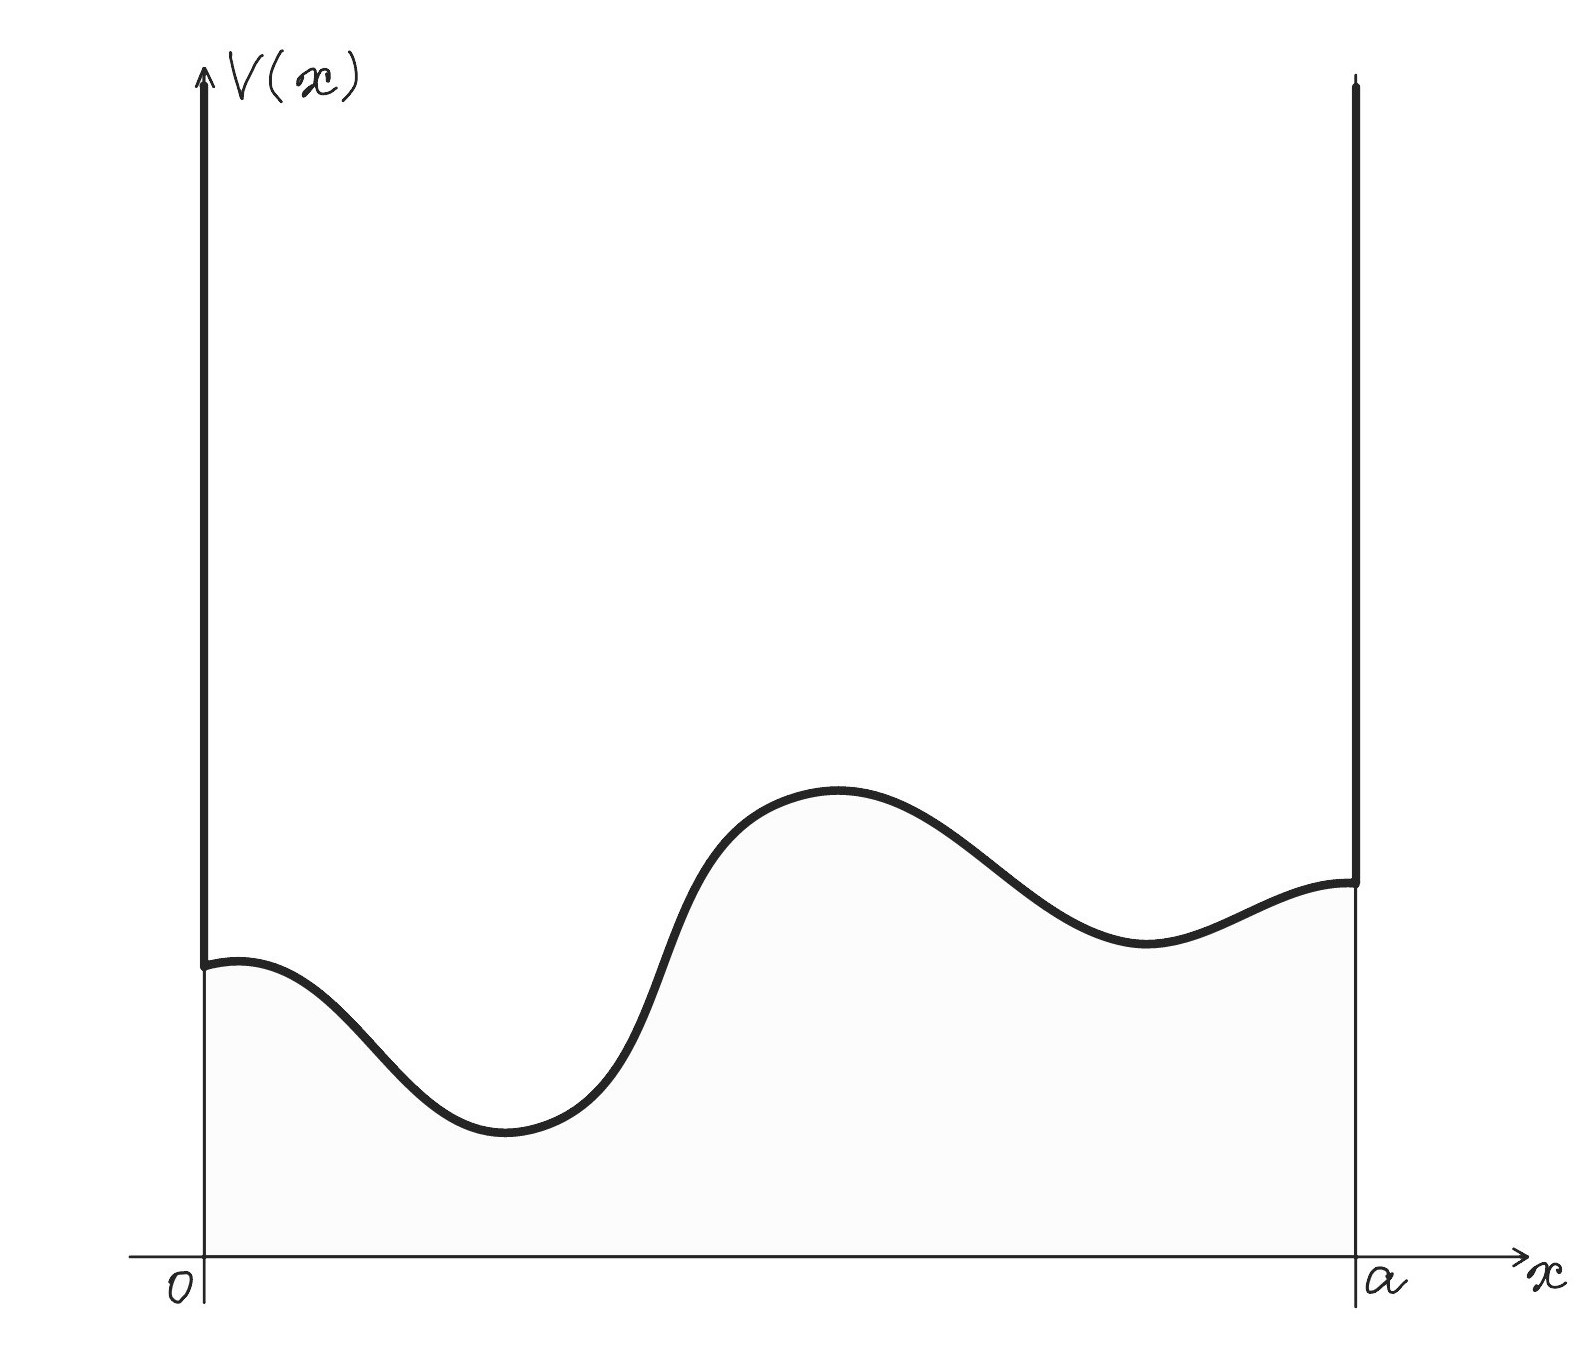
\includegraphics[scale=0.2]{class 11/images/bound-state.jpg}
\caption{Какое-то связанное состояние}
\label{fig 11.1}
\end{figure}
Мы уже решали похожую задачу, однако здесь мы имеем какое-то произвольное дно. Для нас самое главное, чтобы на нём не было резких изменений -- тогда условия квазиклассичности будут соблюдены.

Волновая функция за стенками, очевидно, равна нулю. Внутри ящика мы воспользуемся полученными выражениями:
\[
\psi(x) \simeq \frac{\widetilde{C}_1}{\sqrt{p}}e^{\frac{i}{\hbar}S(x)} + \frac{\widetilde{C}_2}{\sqrt{p}}e^{-\frac{i}{\hbar}S(x)} = \frac{C_1}{\sqrt{p}}\sin (\frac{S(x)}{\hbar}) + \frac{C_2}{\sqrt{p}}\cos(\frac{S(x)}{\hbar}),
\]
где $S(x) = \int\limits_{0}^{x}p\, dx'$. Так как $\psi(0) = 0$, получим, что $C_2 = 0$ (так как $S(0) = 0$). В точке $a \psi(a) = 0$, значит $S(a) = \pi n$, $n = 0, 1, 2, ...$. Тогда
\[
\int\limits_{0}^{a}p\, dx = \pi n \hbar
\]
С помощью этого выражения можно находить приближённые значения энергии. Давайте посмотрим на случай, когда дно ровное (то есть V(x)=0 -- константная функция). В таком случае интеграл от импульса равен $\int\limits_{0}^{a}p\, dx = \int\limits_{0}^{a}\sqrt{2mE} = a\sqrt{2mE}$. Подставляя его в полученное выражение, выразим энергию:
\[
E = \frac{n^2\pi^2\hbar^2}{2ma^2}
\]
Результат получился такой же, как и при честном решении уравнения Шрёдингера. Это отлично!
\csquare{darklavender}

\begin{figure}[ht]
\centering
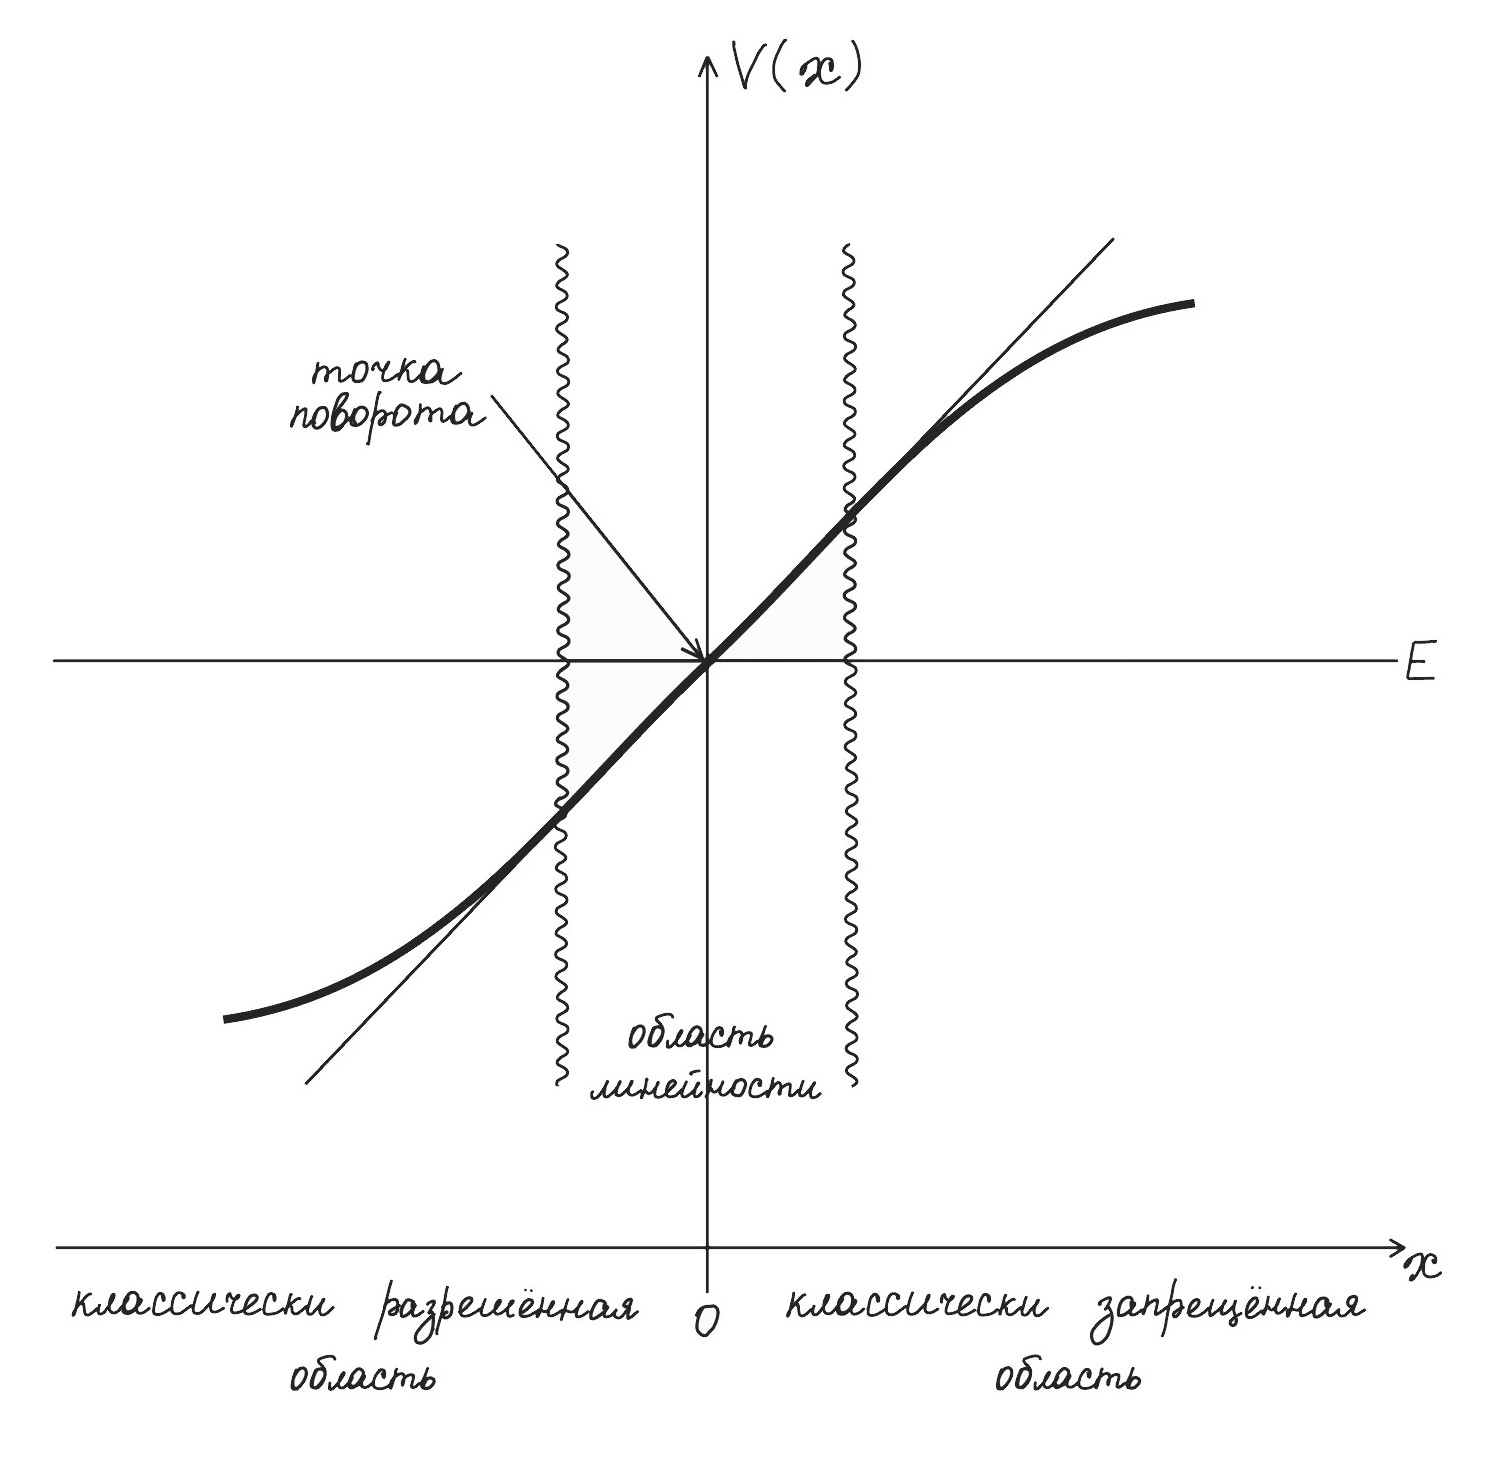
\includegraphics[scale=0.28]{class 11/images/turning-point.jpg}
\caption{Линейное приближение потенциала.}
\label{fig 11.2}
\end{figure}

Теперь эти два решения нужно каким-то образом объединить. Сложность здесь состоит в том, что вблизи точек поворота импульс частицы в классическом случае стремится к нулю и применение квазиклассического приближения становится невозможным. Поэтому приходиться решать уравнение Шрёдингера ``честно''.\footnote{Здесь, в отличие от Ландау, я не буду уходить в ``методически более поучительный'' вариант, так как он привлекает знания ТФКП, которых после сдачи экзамена остаётся не так уж и много. Давайте лучше решать диффуры, это у нас хорошо получается.} Так как мы рассматриваем потенциал достаточно близко к точкам поворота (см. рисунок \ref{fig 11.2}), давайте аппроксимируем наш потенциал прямой линией, используя разложение Тейлора:
\[
V(x) \simeq E + V'(0)x,\; E = V(0)
\]
Подставим этот потенциал в уравнение Шрёдингера:
\[
-\frac{\hbar^2}{2m}\frac{d^2 \psi_T}{dx^2} + [E + V'(0)x]\psi_T = E\psi_T
\]
или
\[
\frac{d^2 \psi_T}{dx^2} = \alpha^3 x \psi_T, \, \alpha = \left[ \frac{2m}{\hbar} V'(0) \right]^{1/3}
\]
Здесь я ввёл обозначение $\psi_T$ для уточнения, что это волновая функция в окрестности точки поворота. Тогда, введя новую переменную $z = \alpha x$, получим \textit{уравнение Эйри}:
\[
\frac{d^2 \psi_T}{dz^2} = z\psi(x)
\]
Решением этого уравнение будут функции Эйри:
\[
\psi_T(x) = aAi(z) + bBi(z)
\]
Подробнее про решение этого уравнения и сами функции можно почитать в третьем томе Ландау, в математических дополнениях. Я не буду вдаваться в это слишком подробно, выпишу лишь основные свойства функций, которые нам понадобятся.

Интегральный вид функций Эйри:
\[
Ai(z) = \frac{1}{\pi}\int\limits_{0}^{\infty}\cos(\frac{s^3}{3} + sz)ds; \quad Bi(z) = \frac{1}{\pi}\int\limits_{0}^{\infty}\left[e^{\frac{-s^3}{3} + sz} + \sin(\frac{s^3}{3} + sz)\right]ds;
\]

Асимптотики:
\[
\begin{rcases}
    Ai(z) \sim \frac{1}{2\sqrt{\pi}z^{1/4}}e^{-\frac{2}{3}z^{3/2}}\\
    Bi(z) \sim \frac{1}{\sqrt{\pi}z^{1/4}}e^{\frac{2}{3}z^{3/2}}
\end{rcases}
 z \gg 0;\quad
 \begin{rcases}
    Ai(z) \sim \frac{1}{\sqrt{\pi}(-z)^{1/4}}\sin\left[\frac{2}{3}(-z)^{3/2} + \frac{\pi}{4}\right]\\
    Bi(z) \sim \frac{1}{\sqrt{\pi}(-z)^{1/4}}\cos\left[\frac{2}{3}(-z)^{3/2} + \frac{\pi}{4}\right]
\end{rcases}
z\ll 0
\]

Теперь мы знаем, как выглядит волновая функция, которая поможет нам объединить две области -- классически запрещённую (слева) и классически разрешенную (справа). Найдём волновую функцию справа. Сначала запишем общий вид волновой функции вне области точки поворота. 
\[
\psi(x) \simeq
\begin{cases}
    \frac{1}{\sqrt{p}}\left[B\exp\left(\frac{i}{\hbar}\int\limits_x^{0}p dx'\right) + C\exp\left(-\frac{i}{\hbar}\int\limits_x^{0}p dx'\right)\right],\; \text{при } x < 0\\
    \frac{1}{\sqrt{|p|}}\left[D\exp\left(-\frac{1}{\hbar}\int\limits_0^{x}|p| dx'\right)\right],\; \text{при } x > 0
\end{cases}
\]
Возьмём область достаточно далёкую от точки поворота, чтобы можно было воспользоваться квазиклассическим приближением, и при этом достаточно близкую, чтобы потенциал был линейный. Тогда:
\[
p(x) \simeq \sqrt{2m (E - E - V'(0)x)} = \hbar\alpha^{3/2}\sqrt{-x}
\]
Тогда для запрещённой области будет выполняться:
\[
\int\limits_{0}^{x}|p|dx' \simeq \hbar\alpha^{3/2}\int\limits_{0}^{x} \sqrt{x'}dx' = \frac{2}{3}\hbar(\alpha x)^{3/2}
\]
Подставляя это в волновую функцию, получим:
\[
\psi(x) \simeq \frac{D}{\sqrt{\hbar}\alpha^{3/4}x^{1/4}}e^{-\frac{2}{3}(\alpha x)^{3/2}}
\]
Возвращаясь к волновой функции у точки поворота, воспользуемся асимптотикой для больших значений z\footnote{Возможность использовать такую аппроксимацию может показаться странной, так как при z=0 мы находимся к точке поворота очень близко. Но, на практике, такое решение имеет место, так как и значение $\alpha x$ достаточно большое, и потенциал ещё линейный. Конкретные значения можно увидеть в \nameref{appendix:C} в первой задаче.}. Тогда её вид в правой области будет следующий:
\[
\psi_T \simeq \frac{a}{2\sqrt{\pi} (\alpha x)^{1/4}}e^{-\frac{2}{3}(\alpha x)^{3/2}} +  \frac{b}{\sqrt{\pi} (\alpha x)^{1/4}}e^{\frac{2}{3}(\alpha x)^{3/2}}
\]
Сравнивая эти волновые функции, мы видим:
\[
a = \sqrt{\frac{4\pi}{\alpha \hbar}}D, \quad b = 0
\]
Проделаем то же самое с областью слева. Посчитаем интеграл от импульса, не забывая, что x теперь отрицательный:
\[
\int\limits_{x}^{0}p\, dx' \simeq \frac{2}{3}\hbar(-\alpha x)^{3/2}
\]
Подставляем в волновую функцию для классически разрешенной области:
\[
\psi(x) \simeq \frac{1}{\sqrt{\hbar}\alpha^{3/4}(-x)^{1/4}}\left[Be^{i\frac{2}{3}(-\alpha x)^{3/2}}+ Ce^{-i\frac{2}{3}(-\alpha x)^{3/2}}\right]
\]
Снова используем асимптотику, но теперь z -- большое отрицательное число, значит и асимптотика будет для $z\ll 0$. Также учитываем, что мы уже нашли коэффициент b -- он равен нулю. Теперь, когда мы ничего не забыли, пишем:
\begin{align*}
\psi_T & \simeq \frac{a}{\sqrt{\pi}(-\alpha x)^{1/4}}\sin\left[\frac{2}{3}(-\alpha x)^{3/2} + \frac{\pi}{4}\right] = \\ & = \frac{a}{\sqrt{\pi}(-\alpha x)^{1/4}}\frac{1}{2i}\left[ e^{i\pi/4}e^{i\frac{2}{3}(-\alpha x)^{3/2}} - e^{-i\pi/4}e^{-i\frac{2}{3}(-\alpha x)^{3/2}}\right]
\end{align*}
Вновь сравнивая функции, получим:
\[
\frac{a}{2i\sqrt{\pi}}e^{i\pi/4} = \frac{B}{\sqrt{\hbar \alpha}}, \quad \frac{-a}{2i\sqrt{\pi}}e^{-i\pi/4} = \frac{C}{\sqrt{\hbar \alpha}},
\]
или, если подставим ранее полученное выражение для $a$:
\[
B = -ie^{i\pi/4}D, \quad C = ie^{-i\pi/4}D
\]
Подставляя эти коэффициенты в первоначальное общее выражение для волновой функции, получим \textit{формулы связи} для области возрастающего потенциала, где $x_2$ -- точка поворота:
\[
\psi_R(x) \simeq 
\begin{cases}
    \frac{2D}{\sqrt{p}}\sin\left[ \frac{1}{\hbar} \int\limits_x^{x_2} p\,dx' + \frac{\pi}{4} \right], \; \text{при } x < x_2\\
    \frac{D}{\sqrt{|p|}}\exp\left[-\frac{1}{\hbar} \int\limits_{x_2}^{x} |p|\,dx' \right],\; \text{при } x > x_2
\end{cases}
\]

Используя тот же самый подход, получим волновую функцию для области убывающего потенциала, где $x_1$ -- точка поворота. Точный расчёт можно посмотреть во второй задаче в \nameref{appendix:C}.
\[
\psi_L(x) \simeq 
\begin{cases}
    \frac{D'}{\sqrt{|p|}}\exp\left[-\frac{1}{\hbar} \int\limits_{x}^{x_1} |p|\,dx' \right],\; \text{при } x < x_1\\
    \frac{2D'}{\sqrt{p}}\sin\left[ \frac{1}{\hbar} \int\limits_{x_1}^{x} p\,dx' + \frac{\pi}{4} \right], \; \text{при } x > x_1\\
\end{cases}
\]
Теперь, когда у нас есть обе волновые функции, вновь рассмотрим потенциальную яму, но теперь у нас нет бесконечных стенок. Рассматривая ``пересекающуюся'' область, волновую функцию для классической области можно записать в виде:
\[
\psi(x) \simeq \frac{2D}{\sqrt{p}}\sin\theta_2(x),\quad \theta_2(x) = \frac{1}{\hbar}\int\limits_{x}^{x_2}p\,dx' + \frac{\pi}{4},
\]
или, используя левую точку поворота:
\[
\psi(x) \simeq \frac{-2D'}{\sqrt{p}}\sin\theta_1(x),\quad \theta_1(x) = -\frac{1}{\hbar}\int\limits_{x_1}^{x}p\,dx' - \frac{\pi}{4}.
\]

Аргументы у синусов должны быть равны по модулю $\pi$, то есть $\theta_2 = \theta_1 + \pi n$. Подставляя полученные выше значения, получим:
\[
\int\limits_{x_1}^{x_2}p\, dx = (n + \frac{1}{2})\hbar\pi,\quad n = 0, 1, 2, ...
\]
Это, так называемое, \textit{правило квантования Бора - Зоммерфельда}. Оно позволяет в случае потенциальных ям с большим значением $n$ найти энергию без решения уравнению Шрёдингера. 

Теперь, имея на руках все инструменты, давайте попробуем решить следующую задачу.
\newpage
\excersize{Упражнение №36}{darklavender}
\begin{center}
    \textit{Найдите энергию и волновые функции для следующих потенциалов:}
    \[
    a)\;V(x) = \frac{m\omega^2 x^2}{2}
    \]
    \[
    b)\;V(x) = 
    \begin{cases}
     \frac{m\omega^2 x^2}{2},\;x > 0\\
    +\infty,\; x < 0
    \end{cases}
    \]
\end{center}

a) Для начала найдём энергию, воспользовавшись правилом Бора-Зоммерфельда. Импульс в нашей задаче равен $p = \sqrt{2mE - m^2\omega^2x^2}$. Точку поворота можно получить, приравняв импульс к нулю и выразив $x$:
\[
x_0 = \sqrt{\frac{2E}{m\omega^2}}
\]
Подставим это в интеграл и посчитаем его:
\begin{align*}
\int\limits_{-x_0}^{x_0}p\;dx & = \int\limits_{-x_0}^{x_0}\sqrt{2mE - m^2\omega^2x^2}\;dx =\\& = \frac{m\omega}{2}\left[x\sqrt{\frac{2E}{m\omega^2}- x^2} + \frac{2E}{m\omega^2}\arctan\left( \frac{x}{\sqrt{\frac{2E}{m\omega^2} - x^2}} \right)\right]\Bigg|_{-x_0}^{x_0} = \\ & = \left( tan^{-1}(+\infty) = \frac{\pi}{2}\right) = 2(\frac{m\omega}{2}\frac{2E}{m\omega^2}\frac{\pi}{2}) = \frac{E\pi}{\omega} = (n + \frac{1}{2})\hbar\pi
\end{align*}
Выражая энергию, получим ожидаемый результат
\[
E_n = \hbar\omega(n + \frac{1}{2})
\]

Теперь найдём волновые функции. Мы знаем, что в аргументе синуса и в показателях экспоненты будут стоять следующие интегралы:
\begin{align*}
I_1 &= \int\limits_{x}^{-x_0}|\sqrt{2mE_n - m^2\omega^2x'^2}|dx'\\
I_2 &= \int\limits_{-x_0}^{x}\sqrt{2mE_n - m^2\omega^2x'^2}dx'\\
I_3 &= \int\limits_{x_0}^{x}|\sqrt{2mE_n - m^2\omega^2x'^2}|dx'
\end{align*}
Посчитаем $I_3$:
\begin{align*}
    I_3 &= \int\limits_{x_0}^{x}|m\omega\sqrt{x_0^2 - x'^2}|dx' = \int\limits_{x_0}^{x}|m\omega\sqrt{x_0^2 - x'^2}|dx' = \\
    &= \frac{m\omega}{2}\left[x'\sqrt{x'^2 - x_0^2} - x_0^2\ln (x' + \sqrt{x'^2 - x_0^2} )\right]\Bigg|_{x_0}^{x} = \\ 
    &= \frac{m\omega}{2}\left[x\sqrt{x^2 - x_0^2} - x_0^2\ln (x + \sqrt{x^2 - x_0^2} ) + x_0^2\ln x_0 \right]= \\
    &= \frac{x_0^2 m\omega}{2} \left[\frac{x}{x_0}\sqrt{\left(\frac{x}{x_0}\right)^2 - 1} - \ln (\frac{x}{x_0} + \sqrt{\left(\frac{x}{x_0}\right)^2 - 1} )\right] = \\
    &=\frac{E_n} {\omega}\left[\frac{x}{x_0}\sqrt{\left(\frac{x}{x_0}\right)^2 - 1} - \ln (\frac{x}{x_0} + \sqrt{ \left(\frac{x}{x_0}\right)^2 - 1} )\right]
\end{align*}
Интеграл $I_1$ будет отличаться от него только знаком:
\begin{align*}
    I_1 = \frac{E_n}{\omega}\left[-\frac{x}{x_0}\sqrt{\left(\frac{x}{x_0}\right)^2 - 1} - \ln (-\frac{x}{x_0} + \sqrt{ \left(\frac{x}{x_0}\right)^2 - 1} )\right]
\end{align*}
Осталось посчитать $I_2$:
\begin{align*}
    I_2 &= \int\limits_{-x_0}^{x}m\omega\sqrt{x_0^2 - x'^2}dx' = \\
    & = \frac{m\omega}{2}\left[x\sqrt{x_0^2- x^2} + x_0^2\arcsin\left(\frac{x}{x_0}\right)\right]\Bigg|_{-x_0}^{x} = \\
    & = \frac{x_0^2 m\omega}{2}\left[\frac{x}{x_0}\sqrt{1 - \left(\frac{x}{x_0}\right)^2 } + \arcsin\left(\frac{x}{x_0}\right) - \arcsin(-1)\right] = \\
    & = \frac{E_n}{\omega}\left[\frac{x}{x_0}\sqrt{1 - \left(\frac{x}{x_0}\right)^2} + \arcsin(\frac{x}{x_0}) + \frac{\pi}{2}\right]
\end{align*}


Подставив эти интегралы, получим волновую функцию в квазиклассическом приближении:
\begin{equation*}
\psi_n(x) = 
\begin{cases}
    \frac{C}{\sqrt{|p|}}e^{-\frac{1}{\hbar}I_1},\; x < -x_0\\
    \frac{C}{\sqrt{p}}\sin(\frac{1}{\hbar}I_2 + \pi/4),\; -x_0 < x < x_0\\
    \frac{C}{\sqrt{|p|}}e^{-\frac{1}{\hbar}I_3},\; x > x_0
\end{cases}
\end{equation*}
Коэффициент $C$ находится из нормировки.

b) Такой потенциал представляет собой правую половину потенциала, рассмотренного нами выше. Значит, в правой части волновая функция будет частично совпадать с волновой функцией из предыдущей задачи. Осталось определить, какой чётностью будет обладать эта часть волновой функции. Для этого воспользуемся граничным условием: $\psi(0) = 0$. Тогда классическая часть квазиклассического приближения волновой функции в той же точке так же должна быть равна нулю:
\[
\sin\left(\frac{1}{\hbar}\int\limits_0^{x_0} p dx + \pi/4 \right) = 0
\]
Тогда, для такой задачи получаем модифицированное правило Бора-Зоммерфельда:
\[
\int\limits_0^{x_0} p dx = \pi\hbar\left(n +\frac{3}{4} \right)
\]
Отсюда, энергия равна:
\[
E_n = \hbar\omega(2n + \frac{3}{2})
\]

Видим, что у нас получились только нечётные значения энергии. Значит, и волновая функция имеет только нечётную часть:
\[
\psi_n(x) =
\begin{cases}
    \sqrt{2}\psi_{2n+1}(x), \; x > 0\\
    0, \; x < 0
\end{cases}
\]
\csquare{darklavender}
    \newpage
    
    \appendix
    \setcounter{figure}{0}  
\begin{center}
    \section{Приложение А}\label{appendix:A}
    \textbf{\Large{Нахождение собственных функций операторов $\hat{L}^2$ и $\hat{L}_z$}.}
\end{center}
Найдём волновые функции состояния $\ket{lm}$. Для начала напишем вид операторов повышения и понижения в координатном базисе
\[
\hat{L}_+ \simeq \hbar e^{i\phi}\left(\frac{\partial}{\partial \theta} + i \ctg\theta\,\frac{\partial}{\partial \phi} \right)
\]
\[
\hat{L}_- \simeq \hbar e^{-i\phi}\left(-\frac{\partial}{\partial \theta} + i \ctg\theta\,\frac{\partial}{\partial \phi} \right)
\]

В каком виде нам искать решения для нашего уравнения? Здесь нам помогут уравнения математической физики и определенные там \textit{сферические функции}. Выпишем их и докажем с помощью математической индукции, что они действительно являются собственными функциями в рассматриваемой системе:
\[
Y^m_l(\theta, \phi) = \mathcal{N}_l\sqrt{\frac{(l+m)!}{(l-m)!}} \frac{1}{\sin^{m}\theta}\,\frac{d^{l-m}}{d(\cos\theta)^{l-m}}\sin^{2l}\theta e^{im\phi},
\]
где $\mathcal{N}_l = (-1)^l \sqrt{\frac{2l+1}{4\pi}}\frac{1}{2^l l!}$ - коэффициент нормирования.

Доказательство построим в 4 шага. Для начала покажем, что при действии оператора повышения на состояние $\ket{ll}$ (то есть $m = l$) мы получим 0. На втором шаге убедимся в том, что правильно определили нормирующий множитель. На третьем шаге применим к сферической функции при $l=m$ оператор $\hat{L}^2$ и убедимся, что функции являются собственными с собственным значением $\hbar^2(l+1)l$. И на последнем шаге сделаем шаг математической индукции: предположим, что состояние $\ket{lm}$ задаётся сферической функцией и покажем, что состояние $\ket{l, m-1}$ так же задаётся сферической функцией.

\begin{enumerate}
    \item При $m = l$ сферические функции имеют вид 
    \[
    Y^l_l(\theta, \phi) = \mathcal{N}_l\sqrt{(2l)!}\sin^l \theta\, e^{i\phi l}.
    \]
    Подействуем на неё повышающим оператором:
    \begin{align*}
        \hat{L}_+\ket{ll} & \simeq \hbar e^{i\phi}{N}_l\sqrt{(2l)!}\left(\frac{\partial}{\partial \theta} + i \ctg\theta\,\frac{\partial}{\partial \phi} \right)\sin^{l}\theta\,e^{i\phi l} = \\
        & = \hbar e^{i\phi}{N}_l\sqrt{(2l)!}\left( l\cos\theta\sin^{l-1}\theta - l\ctg\theta\sin^l\theta\, e^{i\phi l} \right) \\
        & = 0
    \end{align*}
    \item Для проверки нормировки приравняем скалярное произведение состояния на самого себя к единице:
    \begin{align*}
        \braket{ll} & = \int\limits_0^{2\pi}\int\limits_0^{\pi}|Y^l_l(\theta, \phi)|^2 \sin\theta \, d\theta d\phi = \mathcal{N}^2_l(2l)!\int\limits_0^{2\pi}\int\limits_0^{\pi}\sin^{2l}\theta \sin\theta\,d\theta d\phi \\
        & = (\text{сделаем замену} x = \cos\theta,\, dx = -\sin\theta\,d\theta, \text{проинтегрируем по }\phi) =\\
        & = 2\pi\mathcal{N}^2_l(2l)!\int\limits_{-1}^1 (1-x^2)^l dx.
    \end{align*}
    Вычислим этот интеграл. В квадратурах, к сожалению, не получится - решением будет бета-функция. Но мы люди подкованные, таких страшных слов не испугаемся! Напомню, что бета-функция имеет вид
    \[
    B(x, y) = \int\limits_0^1 t^{x-1}(1-t)^{y-1}dt = \frac{\Gamma(x)\Gamma(y)}{\Gamma(x+y)}
    \]
    Приведём наш интеграл к похожему виду:
    \begin{align*}
        & \int\limits_{-1}^1 (1-x^2)^l dx = 2\int\limits_{0}^1 (1-x^2)^l dx =  (z = x^2,\, dz = 2xdx) = \\
        & = \int\limits_{0}^1 z^{-\frac{1}{2}}(1-z)^l dz = B(1/2,\, l+1) = \frac{\Gamma(1/2)\Gamma(l+1)}{\Gamma(l+3/2)}.
    \end{align*}
    Теперь вспоминаем свойства гамма-функций. Во-первых, если n - целое, то $\Gamma(n+1) = n!$. Во-вторых, $\Gamma(1/2 + n) = \frac{(2n)!}{4^n n!}\sqrt{\pi}$. Если подставить n+1, то получим $\Gamma(3/2 + n) = \frac{(2n+2)!}{4^{n+1} (n+1)!}\sqrt{\pi}$. В-третьих, $\Gamma(1/2) = \sqrt{\pi}$. Воспользовавшись этими свойствами, найдём, чему равен интеграл:
    \begin{align*}
        \int\limits_{-1}^1 (1-x^2)^l dx = \frac{\Gamma(1/2)\Gamma(l+1)}{\Gamma(l+3/2)} = 4^{l+1}\frac{(l+1)!\sqrt{\pi}l!}{\sqrt{\pi}(2l+2)!} = 2^{2l + 1}\frac{(l!)^2}{(2l+1)!}
    \end{align*}
    Подставив это выражение, получим
    \begin{align*}
         & 2\pi\mathcal{N}^2_l(2l)!\int\limits_{-1}^1 (1-x^2)^l dx = 2\pi\mathcal{N}^2_l(2l)!\frac{2^{2l+1}(l!)^2}{(2l+1)!}. = \\
         & = 4\pi\mathcal{N}^2_l\frac{2^{2l}(l!)^2}{(2l+1)} = 1\; => \;\mathcal{N} = \sqrt{\frac{{2l+1}}{4\pi}}\frac{1}{2^ll!}
    \end{align*}
    Обычно перед коэффициентом нормирования добавляют $(-1)^{l}$.
    \item Посчитаем $\hat{L}^2\ket{ll}$. Напомню, что оператор $\hat{L}^2$ в координатном базисе имеет вид 
    \[
    \hat{L}^2 \simeq -\hbar^2\left[\frac{1}{\sin\phi}\frac{\partial}{\partial \theta}\left( \sin\theta\frac{\partial}{\partial \theta} \right) + \frac{1}{\sin^2\theta}\frac{\partial^2}{\partial\phi^2}\right]
    \]
    Тогда, подставляя его в выражение, получим:
    \begin{align*}
        \hat{L}^2\ket{ll} & \simeq  -\mathcal{N}_l\sqrt{(2l)!}\hbar^2\left[\frac{1}{\sin\theta}\frac{\partial}{\partial \theta}\left( \sin\theta\frac{\partial}{\partial \theta}\sin^l\theta \right)e^{i\phi l} + \sin^l\theta\frac{1}{\sin^2\theta}\frac{\partial^2}{\partial\phi^2} e^{i\phi l}\right] =\\
        & =  -\mathcal{N}_l\sqrt{(2l)!}\hbar^2\left[\frac{1}{\sin\theta}\frac{\partial}{\partial \theta}\left( l\cos\theta\sin^l\theta \right)e^{i\phi l} - l^2\sin^{l-2}\theta e^{i\phi l}\right] = \\
        & = -\mathcal{N}_l\sqrt{(2l)!}\hbar^2\left[\frac{l}{\sin\theta}\left(-\sin^{l+1}\theta + l\cos^2\theta\sin^{l-1}\theta\right) - l^2\sin^{l-2}\theta\right]e^{i\phi l} = \\
        & = -\mathcal{N}_l\sqrt{(2l)!}\hbar^2\left[-l\sin^{l}\theta + l^2\cos^2\theta\sin^{l-2}\theta - l^2\sin^{l-2}\theta\right]e^{i\phi l} = \\
        & = -\mathcal{N}_l\sqrt{(2l)!}\hbar^2\left[-l\sin^{l}\theta - l^2\sin^{l}\theta \right]e^{i\phi l} = \mathcal{N}_l\sqrt{(2l)!}\hbar^2\left[l(l + 1)\sin^l \theta \right]e^{i\phi l} = \\
        & = \hbar^2l(l+1)Y^l_l(\theta, \phi).
    \end{align*}
    Получилось как раз что нам нужно было: $\hat{L}^2 \ket{ll} = \lambda \ket{ll}$. На этом моменте мы подтвердили базу индукции.
    \item Осталось сделать шаг индукции. Пусть $\ket{lm}$ представим в виде сферической функции. Докажем, что $\ket{l,\, m-1}$ тоже имеет такой вид. Для этого подействуем на состояние $\ket{lm}$ понижающим оператором. Напомню, что в 8 семинаре мы показали, что состояние $\hat{L}_{\pm}\ket{lm}$ является собственным для операторов $\hat{L}^2$ и $\hat{L}_z$. Это позволяет нам спокойной использовать его для доказательства при переходе.
    \begin{align*}
        &\hat{L}_-\ket{lm} \simeq \hbar e^{-i\phi}\mathcal{N}_l\sqrt{\frac{(l+m)!}{(l-m)!}}\left(-\frac{\partial}{\partial \theta} + i \ctg\theta\,\frac{\partial}{\partial \phi} \right)  \frac{1}{\sin^{m}\theta}\,\frac{d^{l-m}}{d(\cos\theta)^{l-m}}\sin^{2l}\theta e^{im\phi} = \\
        & = (\frac{\partial}{\partial \theta} =  -\sin\theta\frac{\partial}{\partial\cos\theta}) = \hbar e^{-i\phi}\mathcal{N}_l\sqrt{\frac{(l+m)!}{(l-m)!}}\biggl(m\ctg\theta\sin^{-m}\theta\frac{d^{l-m}}{d(\cos\theta)^{l-m}}\sin^{2l}\theta + \\
        & + \sin^{-m}\theta(\sin\theta)\frac{d^{l-m+1}}{d(\cos\theta)^{l-m+1}} \sin^{2l}\theta - m\ctg\theta\sin^{-m}\theta\frac{d^{l-m}}{d(\cos\theta)^{l-m}} \sin^{2l}\theta \biggl)e^{im\phi} = \\
        & = \hbar\mathcal{N}_l\sqrt{\frac{(l+m)!}{(l-m)!}}\left( \sin^{-m+1}\frac{d^{l-m+1}}{d(\cos\theta)^{l-m+1}} \sin^{2l}\theta  \right)e^{i\phi(m-1)} = \\
        & =\hbar Y^{m-1}_l(\theta, \phi)\sqrt{(l+m)(l-m+1)}.
    \end{align*}
    Доказательство закончено.
\end{enumerate}
    \newpage
    \begin{center}
    \section{Приложение B}\label{appendix:B}
    \textbf{\Large{Спин. Математический и физический подход}}
\end{center}

План:
\begin{enumerate}
    \item Опыт Штерна -- Герлаха. Сфера Блоха.
    \item Матрицы для вращения поляризации. SO(3), SU(2) матрицы. Сравнение со спинами.
    \item Матрицы и вектора паули. Вращение спиноров.
    \item Сравнение с квантернионами. Группы и алгебра Клиффорда.
\end{enumerate}

Рассказывать про спин в приложении -- затея крайне непростая, так как его строгое математическое описание требует как минимум страниц 30 и пары-тройки семинаров. В связи с этим, я постараюсь дать базовое описание математики спиноров и физики спина. В конце я оставлю ссылки на источники, используя которые я разбирался в этой достаточно запутанной теме. Если вас заинтересует более глубокое понимание -- обязательно пройдите по ссылкам, посмотрите видео и почитайте книги или статьи по этой теме. 

Говорить мы будем в основном не про сам спин, а про объект, которым его описывают математический -  \textit{спинор}. Однако, я попытаюсь не уходить от основной темы и в случае чего всегда возвращаться к ``физике'' процесса. На этом лирические отступления закончены, давайте преступим к изучению спинов и спиноров.

\subsection{Опыт Штерна -- Герлаха}
\hspace{1em} Наверняка подкованный читатель уже много раз слышал про этот эксперимент, однако для полноты картины я не могу обойти его стороной. Поэтому, если вы уверены, что хорошо понимаете суть опыта и вам не нужно напоминать про причину возникновения такого понятия как спин -- можете спокойно пропустить этот параграф и пойти к следующему.

Опыт состоит в пропускании пучка нейтральных частиц (например, атомов серебра) через неоднородное магнитное поле. Схему установки можно посмотреть на рисунке \ref{fig B.1}. Во время проведения эксперимента главенствовала Боровская модель атома, представляющая собой ядро и крутящиеся вокруг него электроны. Исходя из этой модели, в нейтральных атомах магнитное поле, образованное орбитальным моментом, должно распределяться равномерно, образуя на экране прямую линию. На деле же оказалось, что после вылета из магнита частицы летели только в двух направлениях. Это повлекло за собой следующий вывод -- у частиц есть ``внутренний'' магнитный момент, который ещё и квантуется. Его назвали \textit{спин}, так как сначала было предположение, что электрон крутится вокруг своей оси. В итоге оказалось, что это предположение ошибочное и модель Бора в целом неверна, хотя и даёт правильный вектора понимания устройства атома.
\begin{figure}[h!]
\centering
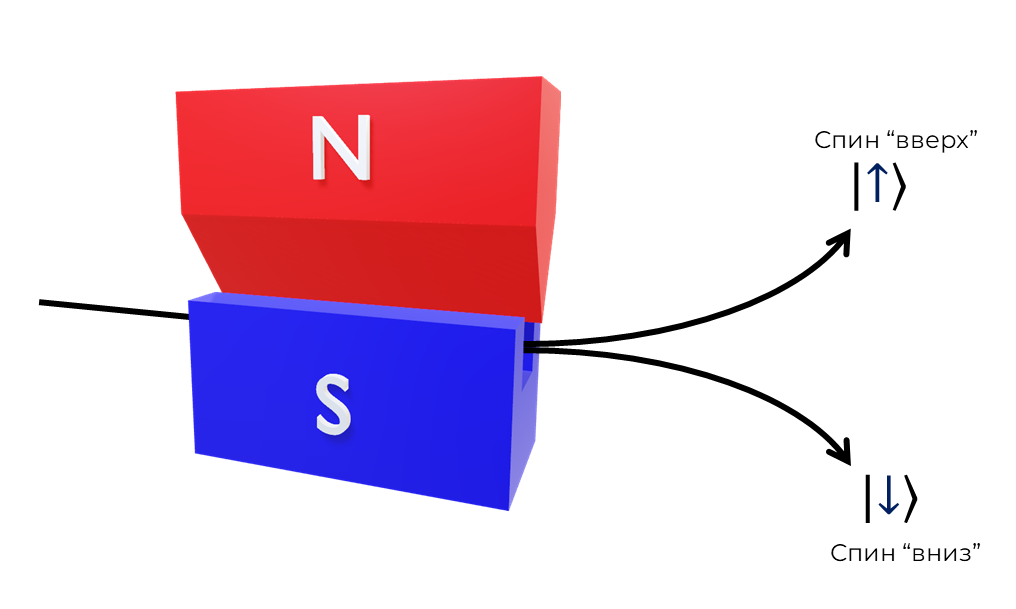
\includegraphics[scale=0.4]{appendix/images/gc.png}
\caption{Магнит с неоднородным магнитным полем. Частицы после вылета попадали на экран.}
\label{fig B.1}
\end{figure}

Итак, у нас есть два состояния - частица летит вверх и частица летит вниз. Пусть вертикальная ось будет ось Z. Обозначим тогда состояние частицы, спин которой направлен "вверх" как $\ket{z}$. Тогда, для частицы со спином вниз будет $\ket{-z}$. Так как частица в момент измерения (т.е. в момент попадания на экран) может оказаться только в одном из состояний, мы считаем, что эти состояния ортогональны. Тогда, если добавить в установку \ref{fig B.1} ещё один магнит, на пути верхней траектории, то частица после второго магнита полетит наверх с вероятностью 1. В формализме квантовой механике это можно записать как:
\[
|\bra{z}\ket{z}|^2 = |\bra{-z}\ket{-z}|^2 = 1,\; |\bra{-z}\ket{z}|^2 = 0
\]
Если мы положим магнит на бок так, что магнитное поле будет направлено вдоль оси X, тогда у нас получится аналогичный результат для состояний $\ket{x}$ и $\ket{-x}$:
\[
|\bra{x}\ket{x}|^2 = |\bra{-x}\ket{-x}|^2 = 1,\;|\bra{-x}\ket{x}|^2 = 0
\]

Разнообразим картину -- пусть подряд идут два магнита, но с разными направлениями. Поставим на пути части, пролетевших первый магнит с состоянием $\ket{z}$, магнит, измеряющий состояние по оси X. Оказывается, вероятность пролететь в ``положительном'' или ``отрицательном'' направлении будет одинаковая и равна 1/2. Другими словами:
\[
|\bra{x}\ket{z}|^2 = |\bra{-x}\ket{z}|^2 = 1/2
\]
Как известно, состояние в квантовой механике можно представить в виде линейной комбинации ``базисных'' состояний. Тогда, разложим состояние $\ket{x}$ как:
\[
\ket{x} = \alpha\ket{z} + \beta\ket{-z}
\]
Из полученной выше вероятности легко найти коэффициенты перед $z$ состояниями:
\[
\ket{x} = \frac{1}{\sqrt{2}}\ket{z} + \frac{1}{\sqrt{2}}\ket{-z}
\]
Из условия ортогональности, получим коэффициенты для состояния $\ket{-x}$:
\[
\ket{-x} = \frac{1}{\sqrt{2}}\ket{z} - \frac{1}{\sqrt{2}}\ket{z}
\]

Для направления по оси Y распределение вероятностей будет точно такое же, как и для оси X. Но те же самые коэффициенты мы взять не можем. Поэтому, чтобы описать состояние $\ket{y}$, будем использовать комплексные числа:
\begin{gather*}
\ket{y} = \frac{1}{\sqrt{2}}\ket{z} + \frac{i}{\sqrt{2}}\ket{-z}\\
\ket{-y} = \frac{1}{\sqrt{2}}\ket{z} - \frac{i}{\sqrt{2}}\ket{-z}
\end{gather*}
Домножение на комплексный множитель не изменяет состояние при измерении, так как берётся квадрат модуля. Поэтому, результаты при подсчёте будут точно такие же.

Обратим внимание на следующий важный момент. Физически состояния $z$ и $-z$ являются антипараллельными, так как частица летит либо вверх, либо вниз. В свою очередь состояния $x$ и $-x$ ортогональный им (рисунок \ref{fig B.2b}). В это же время, соответствующие квантовые состояния имеют следующие отношения: $\ket{z}$ и $\ket{-z}$ ортогональный, а между $\ket{x}$ и $\ket{z}$ угол составляет 45 градусов (рисунок \ref{fig B.2a}). Таким образом, отношение углов между квантовыми состояниями и физическими состояниями соотносится как 1:2. Получается, для полного поворота на 360 градусов в пространстве квантовых состояний необходимо два полных поворота на 720 в физическом пространстве. Это проявление одного из свойств спиноров, о которых мы поговорим далее.

\begin{figure}[!h]
  \centering
  \subfloat[Пространство квантовых состояний]{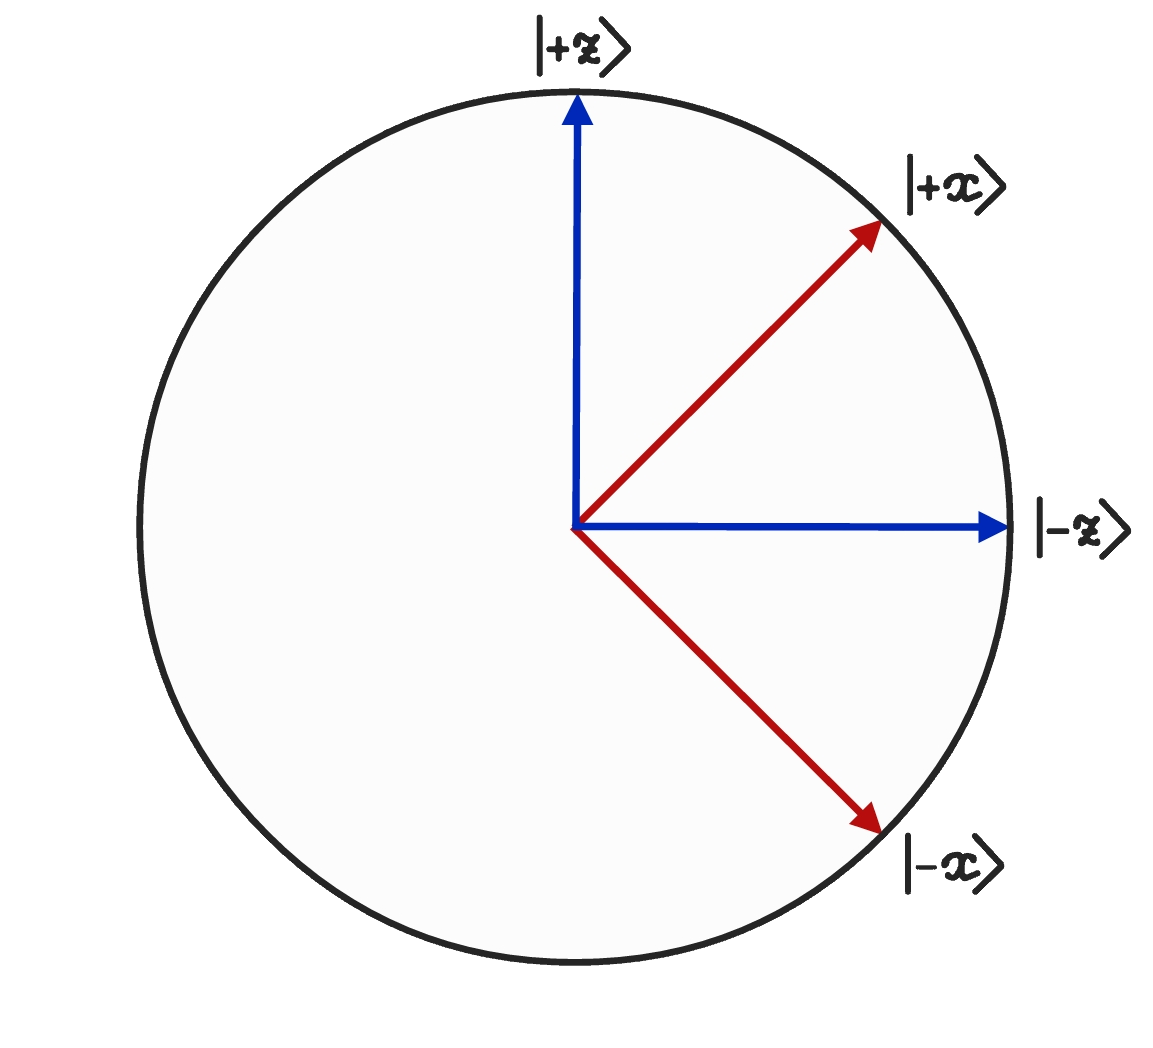
\includegraphics[scale=0.24]{appendix/images/qspace.png}\label{fig B.2a}}
  \hfill
  \subfloat[Физическое пространство]{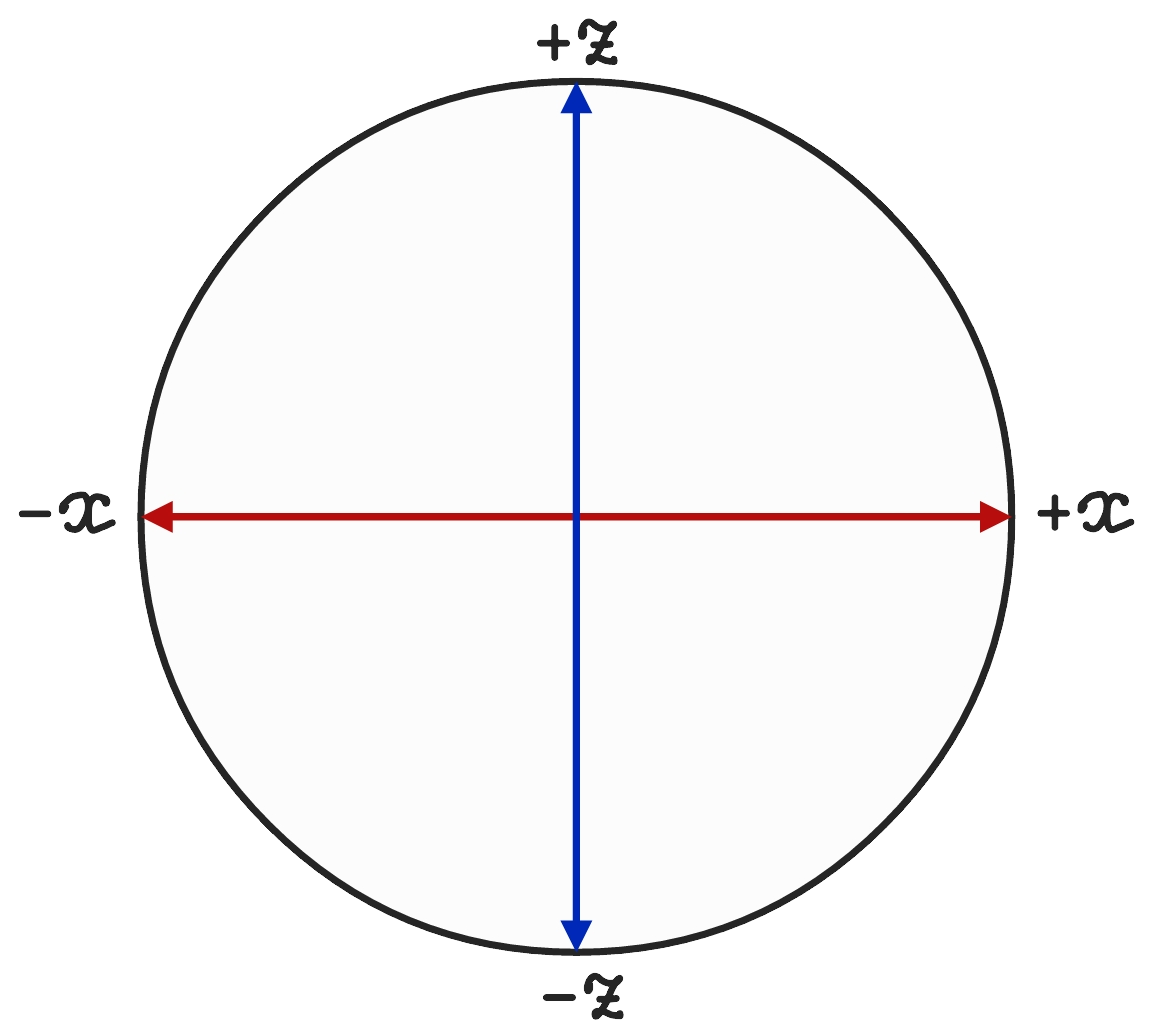
\includegraphics[scale=0.24]{appendix/images/physical space.png} \label{fig B.2b}}
  \caption{}
\end{figure}

В физическом пространстве для представления двухуровневых квантовых состояний используется сфера блоха (рисунок \ref{fig B.3}). Так, состояние $\ket{z}$ можно представить как вектор, направленный вдоль положительной оси Z. Для того, чтобы разобраться, как описывать состояния со спином 1/2 и разобраться со спинорами, нужно обсудить, каким образом вращаются и перемещаются по сфере квантовые состояния. Этим мы и будем заниматься в следующих параграфах.
\begin{figure}[h!]
\centering
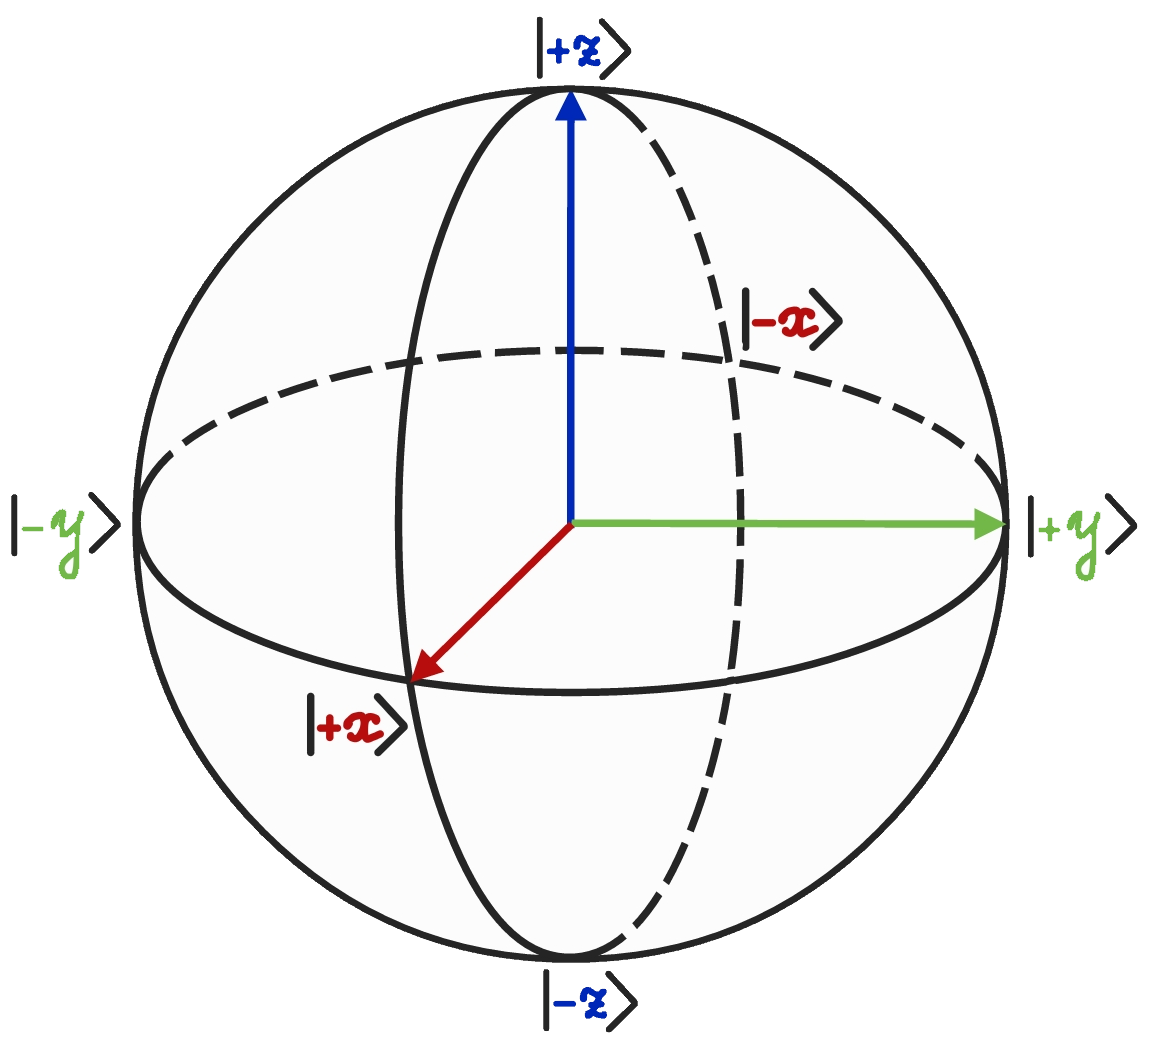
\includegraphics[scale=0.23]{appendix/images/bloch sphere.png}
\caption{Сфера блоха}
\label{fig B.3}
\end{figure}

\subsection{Поляризация света}
Сделаем небольшое отступление от квантовой механики в сторону оптики для того, чтобы укрепить связь между реальной физикой и объектами, используемыми для описания поворота в пространстве. Тем более, с курсом оптики вы уже знакомы, так что многое здесь для вас будет известным и понятным.
\subsubsection{Векторы Джонса}
Поляризацией света можно назвать направление вектора электрического или магнитного поля во время его распространения (рисунок \ref{fig B.4}). Далее в параграфе будем рассматривать только вектор, связанные с электрическим полем. Разложим его в линейную комбинацию трёх базисных векторов:
\[
\Vec{E} = E_x \Vec{e}_x + E_y \Vec{e}_y + E_z \Vec{e}_z
\]
Рассмотрим вертикальную поляризацию. В этом случае $E_z = E_x = 0$. Распишем компоненту $E_y$ :
\[
E_y = A_y \cos(\omega t - kz + \phi_y)
\]
или, используя экспоненциальную форму
\[
E_y = A_y e^{i\phi_y}e^{\omega t - kz}.
\]
Замечу, что если во второй формуле взять реальную часть, получим первую. Так как у нас поляризация реально физическое явление, то в эксперименте мы рассматриваем как раз реальную часть, поэтому такой переход более чем законен.
\begin{figure}[h!]
\centering
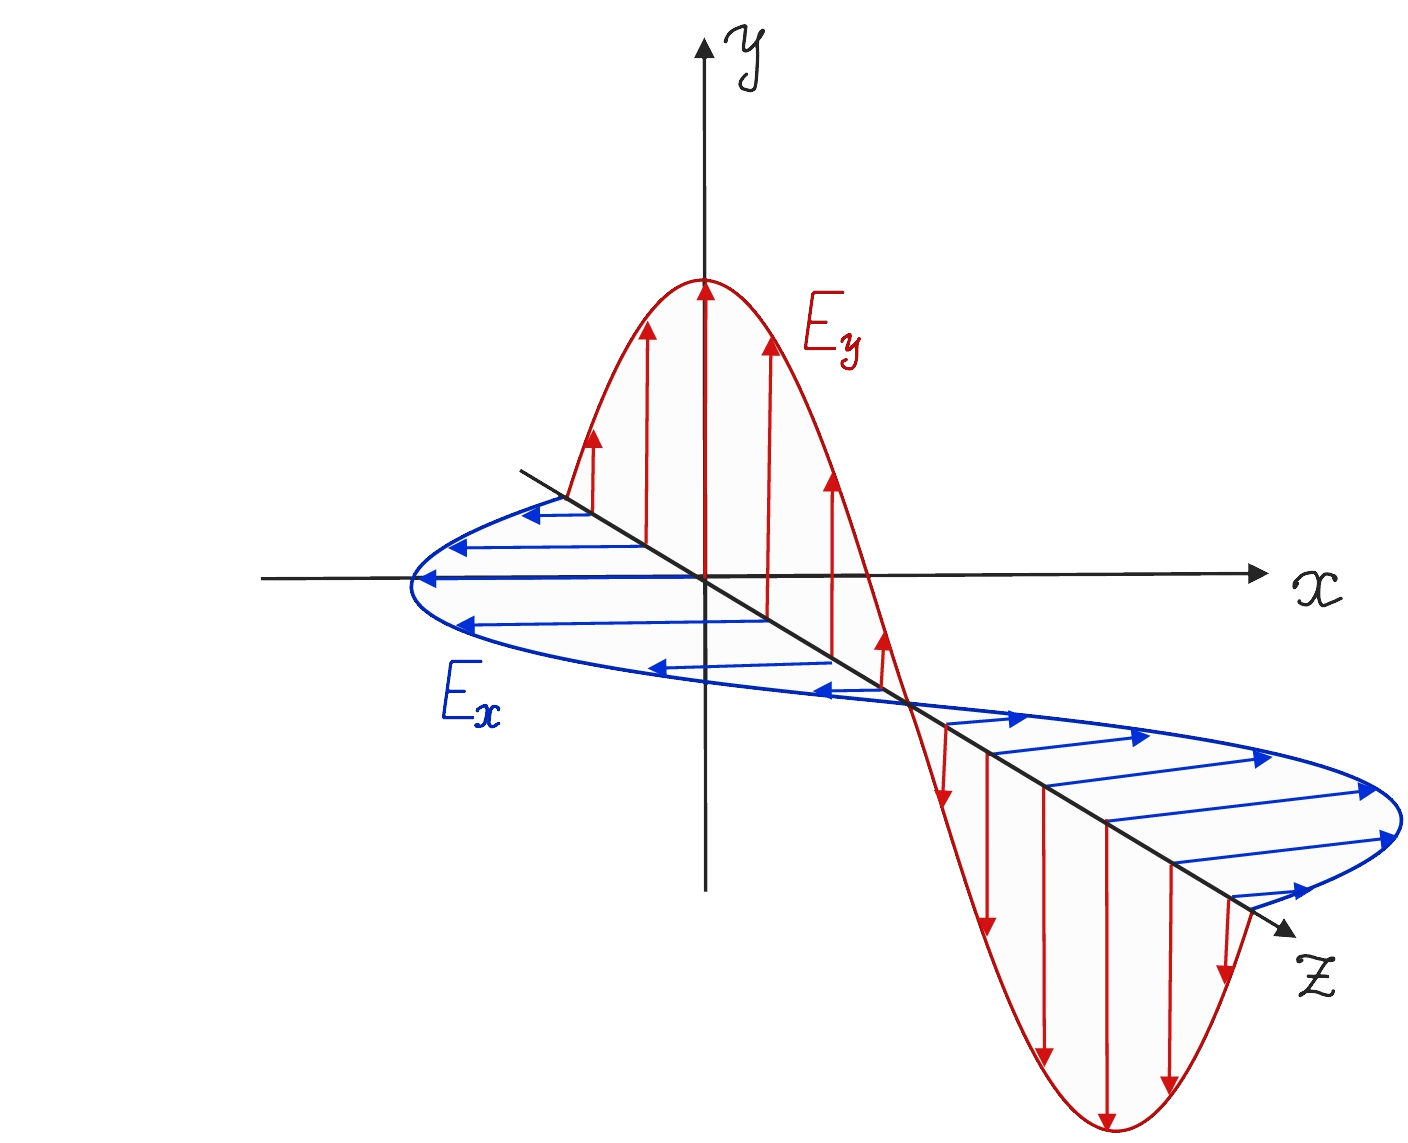
\includegraphics[scale=0.23]{appendix/images/polarization.png}
\caption{Распространение волны вдоль оси Z}
\label{fig B.4}
\end{figure}

Для горизонтальной компоненты аналогично:
\[
E_x = A_x e^{i\phi_x}e^{\omega t - kz}.
\]
Компонента $E_z$ в нашем случае определяет то, в какую сторону будет двигаться волна. Поэтому, мы всегда можем определить координаты так, чтобы эта компонента была равна 0. Тогда, вектор $\Vec{E}$ можно записать в виде
\[
\begin{bmatrix} E_x\\ E_y\\ 0 \end{bmatrix} = \begin{bmatrix} A_x e^{i\phi_x}e^{\omega t - kz}\\ A_y e^{i\phi_y}e^{\omega t - kz}\\ 0 \end{bmatrix}
\]
Легко заметить, что для полного описания поляризации волны нам достаточно знать фазу $\phi$ и амплитуду $A$, так как множитель $e^{\omega t - kz}$ одинаковы для всех членов. Помимо этого, мы можем выкинуть из вектора третий член -- при правильном выборе координат он всегда будет равен 0. Таким образом, мы приходим к \textit{векторам Джонса} -- векторам с двумя членами, описывающими поляризацию волны.
\[
\begin{bmatrix} A_x e^{i\phi_x}e^{\omega t - kz}.\\ A_y e^{i\phi_y}e^{\omega t - kz}\\ 0 \end{bmatrix} \rightarrow \Vec{J} = \begin{bmatrix} A_x e^{i\phi_x}\\ A_y e^{i\phi_y}\end{bmatrix}
\]

Вектор Джонса можно записать в виде линейной комбинации вертикальной и горизонтальной поляризации:
\[
\Vec{J} = A_x e^{i\phi_x}\begin{bmatrix} 1 \\ 0 \end{bmatrix} + A_y e^{i\phi_y}\begin{bmatrix} 0 \\ 1 \end{bmatrix} = A_x e^{i\phi_x}\Vec{H} + A_y e^{i\phi_y}\Vec{V}
\]
Теперь найдём, как используя вектор Джонса описать известные нам диагональную и левую круговую поляризацию. Пусть в обоих членах амплитуда будет равна 1, а фаза равна 0. Тогда, получим сумму двух перпендикулярных векторов с длинной 1. Из прямоугольного треугольника, построенного на этих векторах, находим, что длинна их суммы равна $\sqrt{2}$. Значит, чтобы суммарный вектор получился нормированным, необходимо оба члена разделить на $\frac{1}{\sqrt{2}}$. Назовём его $\Vec{D}$ и запишем его разложение:
\[
\Vec{D} = \frac{1}{\sqrt{2}}\Vec{H} + \frac{1}{\sqrt{2}}\Vec{V}
\]
Ничего не напоминает? Не будем сильно спешить, но я думаю внимательный читатель уже заметил сходство с разложением состояния $\ket{x}$ по базисным состояниям $\ket{z}$ и $\ket{-z}$. Точно также мы можем представить антидиагональную поляризацию $\Vec{A}$, поменяв сумму векторов на разность:
\[
\Vec{A} = \frac{1}{\sqrt{2}}\Vec{H} - \frac{1}{\sqrt{2}}\Vec{V}
\]
Расположение векторов Джонса можно посмотреть на рисунке \ref{fig B.5}
\begin{figure}[h!]
\centering
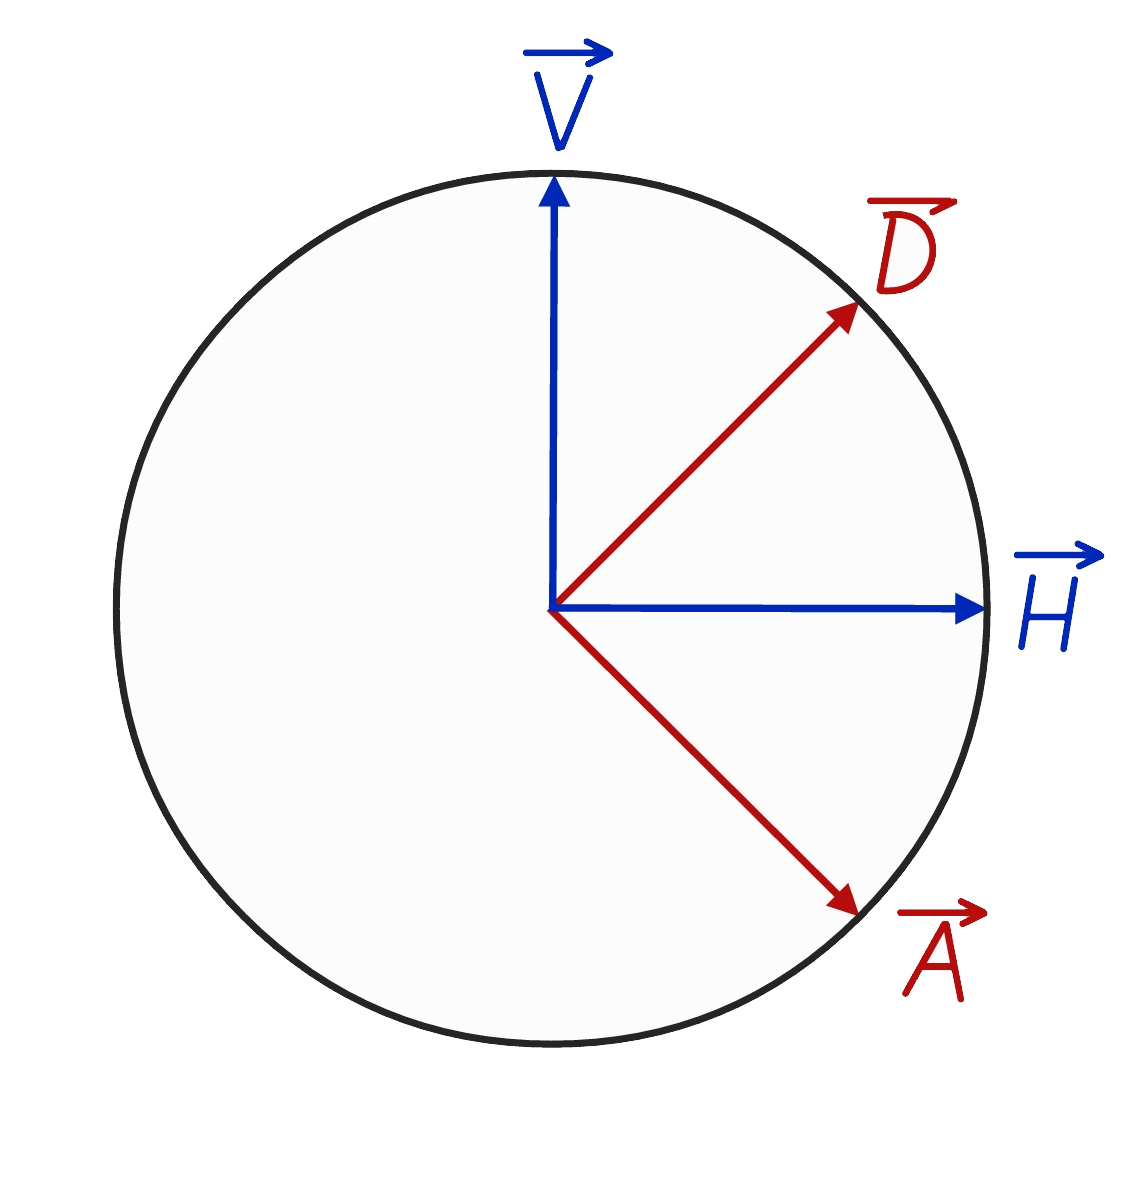
\includegraphics[scale=0.23]{appendix/images/pol phys space.png}
\caption{Расположение векторов Джонса}
\label{fig B.5}
\end{figure}

Рассмотрим ещё одну, более сложную поляризацию. Пусть амплитуда так же равна единице, однако фаза при вертикальной поляризации равна $\pi/2$, то есть:
\[
\Vec{J} = \Vec{H} + e^{i\frac{\pi}{2}}\Vec{V}
\]
Для анализа выберем частоту $\omega = 1$ и $z = 0$. Тогда, вспоминая про наш дополнительный член, который мы вынесли за вектор, можем сделать следующую цепочку преобразований:
\begin{align*}
(\begin{bmatrix} 1 \\ 0 \end{bmatrix} + \begin{bmatrix} 0 \\ e^{i\frac{\pi}{2}} \end{bmatrix})e^{it} = \begin{bmatrix} 1 \\ e^{i\frac{\pi}{2}} \end{bmatrix} e^{it} = \begin{bmatrix} e^{it} \\ e^{i(\frac{\pi}{2} + t)} \end{bmatrix} \rightarrow \begin{bmatrix} \cos t \\ \cos(\frac{\pi}{2} + t) \end{bmatrix} = \begin{bmatrix} \cos t \\ -\sin t \end{bmatrix}
\end{align*}
Подставляя разные значения t, можно заметить, что поляризация вращается по часовой стрелке. Действительно, при $t = 0$ вектор Джонса будет равен $\Vec{H}$, при $t = \frac{\pi}{2}$ вектор равен $-\Vec{V}$ и так далее. Этот вектор будем называть левой круговой поляризацией и обозначать $\Vec{L}$. Ортогональный ему, вектор правой круговой поляризации будем обозначать $\Vec{R}$. Запишем их разложение через вектор $\Vec{H}$ и вектор $\Vec{V}$ сразу с нормировкой:
\begin{gather*}
    \Vec{L} = \frac{1}{\sqrt{2}}\Vec{H} + \frac{i}{\sqrt{2}}\Vec{V}\\
    \Vec{R} = \frac{1}{\sqrt{2}}\Vec{H} - \frac{i}{\sqrt{2}}\Vec{V}
\end{gather*}
Здесь, по формуле Эйлера мы заменили $e^{i\pi/2}$ на $i$.

Итак, как и в случае со спинами, мы нашли 6 состояний, которые описывают любую возможную поляризацию. На самом деле, вектора Джонса ведут себя точно так же, как и спиноры, поэтому являются отличной иллюстрацией последних. В физическом пространстве найденные вектора Джонса между собой ортогональный. Давайте покажем, что в ``поляризационном'' пространстве угол между векторами будет в два раза больше. Для этого посмотрим, как осуществляется переход от одного состояния к другому.
\subsubsection{Матрицы Джонса. Сфера Пуанкаре}
Для вращений векторов Джонса мы используем, как это не удивительно, матрицы Джонса. У них тоже есть физическое воплощение -- волновые пластины. Так, четвертьволновой пластине, которая меняет фазу на $\pi/2$, соответствует матрица $\begin{bmatrix} 1 & 0 \\ 0 & i \end{bmatrix}$. Давайте посмотрим, как она будет действовать на диагональную поляризацию:
\[
\begin{bmatrix} 1 & 0 \\ 0 & i \end{bmatrix}\Vec{D} = \frac{1}{\sqrt{2}}\begin{bmatrix} 1 & 0 \\ 0 & i \end{bmatrix}\begin{bmatrix} 1 \\ 1 \end{bmatrix} = \frac{1}{\sqrt{2}}\begin{bmatrix} 1 \\ i \end{bmatrix} = \Vec{L}
\]
Значит, диагональная поляризация под действием четвертьволновой пластинки переходит в левую круговую поляризацию. Если поставить ещё несколько пластинок, то цепочка переходов будет следующая: $\Vec{D} \rightarrow \Vec{L} \rightarrow \Vec{A} \rightarrow \Vec{R}\rightarrow \Vec{D}$.

Если попробовать подействовать пластинкой на горизонтальную поляризацию, то легко убедиться, что ничего не поменяется. Однако, можно провести трюк -- если повернуть пластину на $45^{\circ}$, то поляризация для неё станет диагональной. С математической точки зрения нам нужно повернуть сначала повернуть базис на $\pi/4$, затем подействовать пластинкой, затем повернуть базис обратно. Запишем матрицу, которая получится при последовательном выполнении этих действий:
\[
\begin{bmatrix} \cos \frac{\pi}{4} & \sin \frac{\pi}{4} \\ -\sin \frac{\pi}{4} & \cos \frac{\pi}{4} \end{bmatrix} \begin{bmatrix} 1 & 0 \\ 0 & i \end{bmatrix} \begin{bmatrix} \cos \frac{\pi}{4} & -\sin \frac{\pi}{4} \\ \sin \frac{\pi}{4} & \cos \frac{\pi}{4} \end{bmatrix} = \frac{1}{2} \begin{bmatrix} 1 + i& -1 + i \\ -1 + i & 1 + i \end{bmatrix} = \frac{1}{\sqrt{2}}\begin{bmatrix} 1 & i \\ i & 1 \end{bmatrix}e^{i\frac{\pi}{4}}
\]
Попробуем применить это преобразование к вектору Джонса $\Vec{H}$, описывающему горизонтальную поляризацию:
\[
e^{i\frac{\pi}{4}}\frac{1}{\sqrt{2}}\begin{bmatrix} 1 & i \\ i & 1 \end{bmatrix}\begin{bmatrix} 1  \\ 0 \end{bmatrix} = e^{i\frac{\pi}{4}}\frac{1}{\sqrt{2}}\begin{bmatrix} 1  \\ i \end{bmatrix} = e^{i\frac{\pi}{4}}\Vec{L}
\]
Результат более чем ожидаемый. Далее я буду опускать фазовый множитель, так как он не влияет на поляризацию. Действительно, домножение элементов вектора Джонса на комплексное значение даст просто смещение волны относительно оси z, однако поляризация останется та же. Осталось определить матрицу для перехода от поляризации $\Vec{H}$ к поляризации $\Vec{A}$:
\[
\frac{1}{\sqrt{2}}\begin{bmatrix} 1 & 1 \\ -1 & 1 \end{bmatrix}\begin{bmatrix} 1  \\ 0 \end{bmatrix} = \frac{1}{\sqrt{2}}\begin{bmatrix} 1  \\ -1 \end{bmatrix}
\]
Теперь у нас есть три матрицы, используя которые мы можем переходить к любой из найденных нами 6 поляризаций. Смотря на цепочки преобразований, можно составить сферу Пуанкаре (рисунок \ref{fig B.6}). По ней видно, что, в отличие от физического пространства, ортогональные поляризации (например $\Vec{H}$ и $\Vec{V}$) находятся под углом $180^{\circ}$ друг к другу. То есть ситуация аналогична ситуации со спинами.
\begin{figure}[h!]
\centering
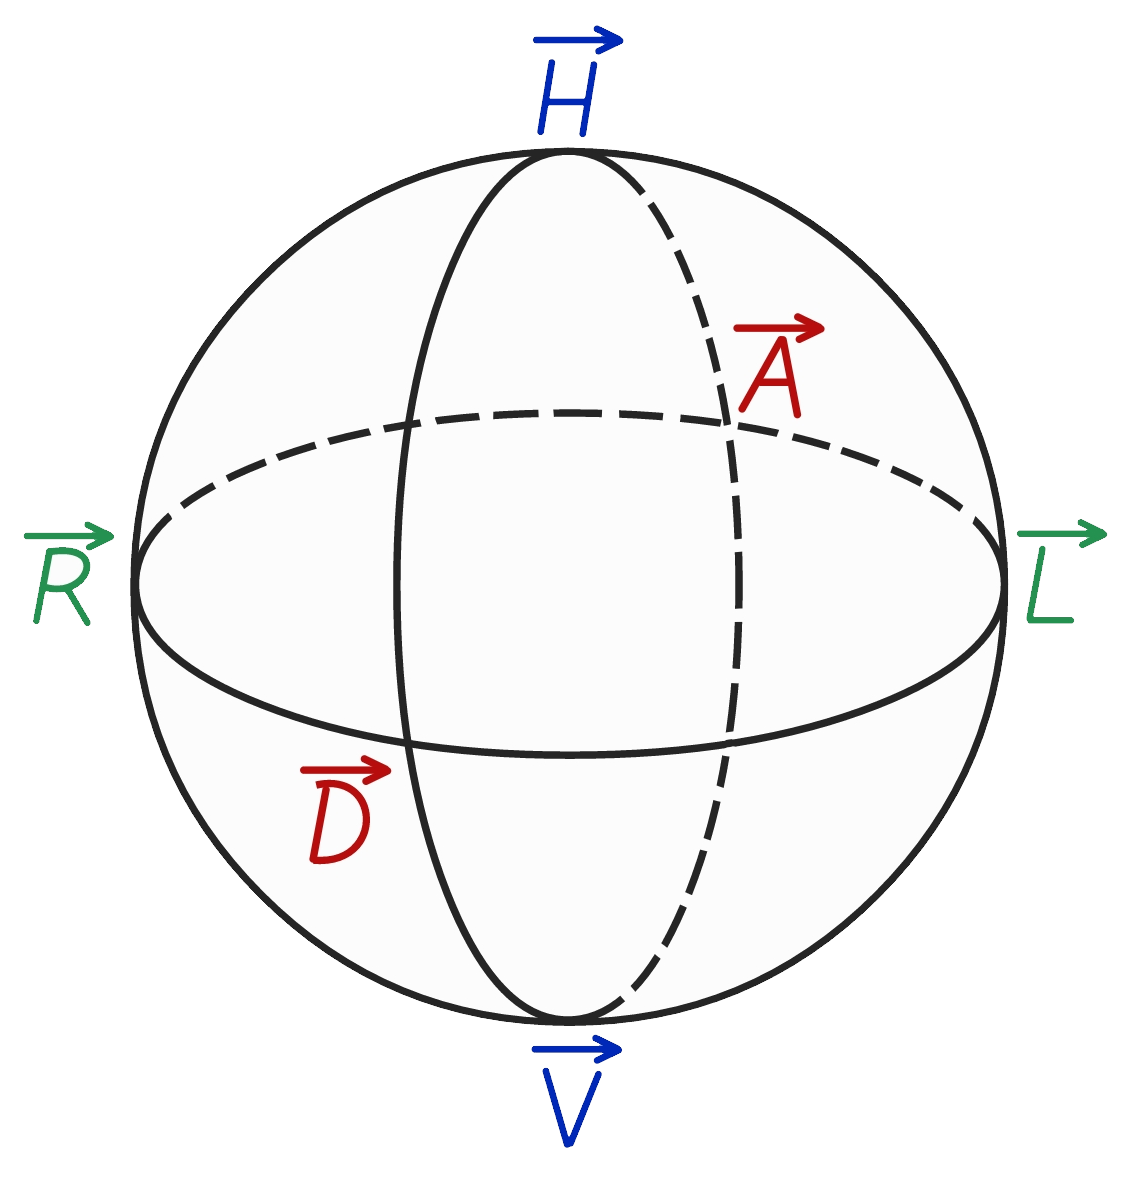
\includegraphics[scale=0.23]{appendix/images/Poincare sphere.png}
\caption{Сфера Пуанкаре}
\label{fig B.6}
\end{figure}

\subsection{Группа вращений SO(3) и SU(2), их связь}
Теперь, когда мы рассмотрели физические примеры спиноров, давайте поговорим про то, каким образом описывается их поворот в пространстве. Для этого вспомним линейную алгебру и разберёмся с ортогональными и унитарными преобразованиями.

Итак, мы хотим поворачивать вектор в трёхмерном пространстве, не изменяя его длины. Так как длина вектора определяется как квадрат нормы, нам необходимо, чтобы выполнялось следующее условие:
\[
\Vec{v} \rightarrow R\Vec{v}, \; ||\Vec{v}||^2 = ||R\Vec{v}||^2
\]
Тогда, записав норму как $v^Tv$, получим ограничение на матрицу $R$:
\[
||\Vec{v}||^2 = \Vec{v}^T\Vec{v} = (R\Vec{v})^T(R\Vec{v}) = \Vec{v}^T R^T R\Vec{v} \implies R^T R = E
\]
Матрицы, удовлетворяющие этому условию, называются ортогональными. Для обозначения множества этих матриц используют $O(3)$ (orthogonal, 3D). Однако, это не все условия, так как отражение тоже не изменяет длину вектора. Для того чтобы отделить вращения от отражения, необходимо посмотреть на детерминант матрицы. 
\begin{align*}
    R^T R = E &\implies \det(R^T)\det(R) = \det(E) \implies [\det(R)]^2 = 1  \\
    &\implies [\det(R)] = \pm 1
\end{align*}
Так как детерминант имеет смысл ориентированного объёма, то понятно, что для вращений нам нужно взять вариант с плюсом. Итак, дополнив условием на детерминант, получим специальную ортогональную группу $S0(3)$.
\[
\begin{cases}
    [\det(R)] = +1\\
     R^T R = E
\end{cases} \implies SO(3)
\]

Группа $S0(3)$ отвечает за вращение векторов в 3D. Но объект нашего изучения -- спиноры, комплексные вектора с двумя элементами. Так как квадрат в для комплексных чисел определяется как произведение комплексное на комплексно сопряженное, мы должны обновить условие для матриц:
\[
||\Vec{J}||^2 = J^{\dagger}J = ||U\Vec{J}||^2 \implies  U^{\dagger}U = E
\]
Такие матрицы называются унитарными. Они образуют группу $U(2)$. С детерминантом ситуация похожая, но чуть более сложная:
\[
|det(U)|^2 = 1 \implies |det(U)| = e^{i\phi}.
\]
Аналогично, выбираем детерминант равный $+1$. Благо мы можем привести любую матрицу к этому детерминанту, так как домножение на комплексный множитель не влияет на спинор. Такая группа, как вы могли догадаться, называется $SU(2)$.
\[
\begin{cases}
    [\det(U)] = +1\\
     U^{\dagger}U = E
\end{cases} \implies SU(2)
\]
Легко удостовериться, что матрицы, которые мы нашли до этого, как раз из $SU(2)$ группы:
\begin{align*}
    \frac{1}{2}\begin{bmatrix} 1 & -1 \\ 1 & 1 \end{bmatrix} \begin{bmatrix} 1 & 1 \\ -1 & 1 \end{bmatrix} = \frac{1}{2} \begin{bmatrix} 2 & 0 \\ 0 & 2 \end{bmatrix} &= E, & \frac{1}{\sqrt{2}}&\begin{vmatrix} 1 & 1\\ -1 & 1\end{vmatrix} = \frac{1}{2} + \frac{1}{2} = 1\\
    \frac{1}{2}\begin{bmatrix} 1 & -i \\ -i & 1 \end{bmatrix}\begin{bmatrix} 1 & i \\ i & 1 \end{bmatrix} = \frac{1}{2}\begin{bmatrix} 2 & 0 \\ 0 & 2 \end{bmatrix} &= E, & \frac{1}{\sqrt{2}}&\begin{vmatrix} 1 & i \\ i & 1 \end{vmatrix} = \frac{1}{2} + \frac{1}{2} = 1\\
    \begin{bmatrix} 1 & 0 \\ 0 & -i \end{bmatrix}\begin{bmatrix} 1 & 0 \\ 0 & i \end{bmatrix} &= E, & e^{-i\frac{\pi}{4}} &\begin{vmatrix} 1 & 0 \\ 0 & i \end{vmatrix} = e^{i(-\frac{\pi}{4} - \frac{\pi}{4} + \frac{\pi}{2})} = 1\\
\end{align*}
Во втором и третьем примерах мы домножили на $e^{-i\frac{\pi}{4}}$. Напомню, что домножение на комплексный множитель не меняет итогового значения поляризации. Благодаря этому факту, можно показать, что состояния в поляризационном пространстве \ref{fig B.6} имеют в два раза больший угол между друг другом чем в физическом пространстве \ref{fig B.5}. Так, выполнив цепочку преобразований $\vec{V} \rightarrow \vec{D} \rightarrow \vec{H} \rightarrow \vec{A} \rightarrow \vec{V}$ мы получим
\begin{align*}
\frac{1}{4}\begin{bmatrix} 1 & 1 \\ -1 & 1 \end{bmatrix}^4\begin{bmatrix} 0 \\ 1 \end{bmatrix} &= \frac{1}{4}\begin{bmatrix} 1 & 1 \\ -1 & 1 \end{bmatrix}^3\begin{bmatrix} 1 \\ 1 \end{bmatrix} = \frac{1}{4}\begin{bmatrix} 1 & 1 \\ -1 & 1 \end{bmatrix}^2\begin{bmatrix} 2 \\ 0 \end{bmatrix} = \\
&=\frac{1}{4}\begin{bmatrix} 1 & 1 \\ -1 & 1 \end{bmatrix}\begin{bmatrix} 2 \\ -2 \end{bmatrix} = \frac{1}{4}\begin{bmatrix} 0 \\ -4 \end{bmatrix} = \begin{bmatrix} 0 \\ -1 \end{bmatrix} = -\vec{V}
\end{align*}
Для описания поляризации этот минус не влияет, так как его можно представить в виде комплексного множителя $e^{i\pi}$. Другими словами, мы сделали полный круг и вернулись в первоначальное состояние. Однако в физическом пространстве мы повернули первоначальный вектор на 180 градусов. Если мы повторим эту цепочку, то придём к $\vec{V}$ в обоих пространствах. Получается, чтобы сделать полный круг в физическом пространстве, нужно сделать два круга для поляризационного пространства.

До этого момента в последних двух параграфах мы говорили только о поляризации и векторах Джонса. На самом деле, все полученные результаты можно перенести на спиновое состояние и спиноры. Действительно, если предположить, что вектор состояния $\ket{z}$ равен $\begin{bmatrix} 1 \\ 0 \end{bmatrix}$, а $\ket{-z}$ равен $\begin{bmatrix} 0 \\ 1 \end{bmatrix}$, то для оставшихся состояний получатся те же самые результаты. Последние рассуждения также можно перенести на спиновое пространство -- для полного поворота вектора спина в пространстве квантовых состояний нам необходимо два поворота в физическом пространстве.\\
У тех, кто читал 8 семинар, может возникнуть закономерный вопрос: а где здесь матрицы Паули? Тем более, что они сами по себе хоть и унитарны, но не являются элементами $SU(2)$ группы. Действительно, детерминант всё трёх матриц Паули не будет равен $+1$. Значит, мы не можем с их помощью вращать спин? Это правда, но только отчасти.
\subsection{Векторы и матрицы Паули}
Давайте вспомним, что такое матрицы Паули. Для этого запишем их явный вид и посмотрим на их свойства. Свойства я буду проверять на одном примере, оставшиеся случаи можно проверить самостоятельно.
\[
\sigma_x = \begin{bmatrix} 0 & 1 \\ 1 & 0 \end{bmatrix}, \quad \sigma_y = \begin{bmatrix} 0 & -i \\ i & 0 \end{bmatrix}, \quad \sigma_z = \begin{bmatrix} 1 & 0 \\ 0 & -1 \end{bmatrix}
\]
Во-первых, они унитарны и эрмитовы. Действительно
\[
\sigma_z^{\dagger}\sigma_z = \begin{bmatrix} 1 & 0 \\ 0 & -1 \end{bmatrix}\begin{bmatrix} 1 & 0 \\ 0 & -1 \end{bmatrix} = E
\]
Отсюда следует, что квадрат любой матрицы Паули будет равен единичной матрице.
\[
\sigma_i^2 = E
\]
Во-вторых, матрицы Паули антикоммутируют друг с другом. Проверим:
\begin{align*}
    \sigma_y\sigma_z = \begin{bmatrix} 0 & -i \\ i & 0 \end{bmatrix}&\begin{bmatrix} 1 & 0 \\ 0 & -1 \end{bmatrix} = \begin{bmatrix} 0 & i \\ i & 0 \end{bmatrix}\\
    \sigma_z\sigma_y = \begin{bmatrix} 1 & 0 \\ 0 & -1 \end{bmatrix}&\begin{bmatrix} 0 & -i \\ i & 0 \end{bmatrix} = \begin{bmatrix} 0 & -i \\ -i & 0 \end{bmatrix}\\
    \sigma_y\sigma_z &= -\sigma_z\sigma_y
\end{align*}
В общем случае можно записать это свойство, используя скобки антикоммутации.
\[
\{\sigma_i,\sigma_j\} = 0, \; i\neq j
\]
Последнее свойство, которое нам понадобится позже, это нулевой след:
\[
\Tr(\sigma_z) = 1 - 1 = 0
\]
или в общем случае
\[
\Tr(\sigma_i) = 0
\]

Так как матрицы Паули унитарны, мы можем использовать их для вращения состояний, описываемых векторами с комплексными элементами. Но, мы знаем, что вращениям соответствуют матрицы с детерминантом +1, в то время как для отражений детерминант матриц равен -1. Несложно убедиться, что детерминант матриц Паули равен как раз -1:
\[
\det(\sigma_z) = \begin{vmatrix} 1 & 0 \\ 0 & -1 \end{vmatrix} = -1 
\]
Получается, действие матриц Паули соответствует отражению вектора. Перед нами сейчас стоит две задачи: разобраться, на как выглядит вектор, на который действуют матрицы Паули и как с помощью них осуществлять именно поворот. Пойдём по порядку.

Как известно, любой вектор можно представить в виде линейной комбинации базисных векторов. Попробуем сделать это, но вместо базисных векторов возьмём матрицы Паули:
\begin{align*}
V = x\sigma_x + y\sigma_y + z\sigma_z = \begin{bmatrix} 0 & x \\ x & 0 \end{bmatrix} + \begin{bmatrix} 0 & -iy \\ iy & 0 \end{bmatrix} + \begin{bmatrix} z & 0 \\ 0 & -z \end{bmatrix} = \begin{bmatrix} z & x-iy \\ x+iy & -z \end{bmatrix}
\end{align*}
Получившийся вектор будем называть вектором Паули.
\subsection{Матрицы Паули как элементы алгебры Клиффорда}
    \newpage
    \begin{center}
    \section{Приложение С}\label{appendix:C}
    \textbf{\Large{Раскрытие некоторых математических аспектов квазиклассики на примере задач.}}
\end{center}

\excersize{Упражнение №C1}{darklavender}
\begin{center}
\textit{Пусть частица массой m находится на n-ом уровне гармонического осциллятора. Найдите точку поворота $x_2$. Насколько далеко от точки поворота может улететь частица перед тем как ошибка из-за линеаризации потенциала достигнет 1\%?}.\\
\textit{При $z\geq 5$ применение асимптотики для функции Эйри $Ai(z)$ даёт ошибку в 1\%. Для расстояния вылета за точку поворота d найти наименьший уровень n, при котором $\alpha d\geq 5$}.
\end{center}
Напомню, как выглядит энергия для квантового гармонического осциллятора: 
\[E_n = \hbar\omega(n + 1/2).\] Точку поворота можно найти из условия p = 0:
\begin{gather*} 
p(x_2) = \sqrt{2mE_n - m^2\omega^2x_2^2} = 0\; => \; 2mE_n = m^2\omega^2x_2^2 \; => \\
=>\; x_2 = \sqrt{\frac{(2n + 1)\hbar}{m\omega}}
\end{gather*}
Пусть d -- искомое расстояние, на которое может улететь частица при сохранении ошибки в 1\%. Тогда найдём d из следующей формулы:
\[
\frac{V(x_2 + d) - V_{lin}(x_2 + d)}{V(x_2)} = 0.01
\]
Найдём $V_{lin}(x_2 + d)$:
\begin{gather*}
V_{lin}(x) = V(x_2) + V'(x_2)(x - x_2) = \frac{m\omega^2 x_2^2}{2} + (m\omega^2 x_2)(x-x_2)\; => \;\\
V_{lin}(x_2 + d) = \frac{m\omega^2 x_2^2}{2} + m\omega^2 x_2d.
\end{gather*}
Подставив это в формулу, получим:
\begin{gather*}
    \frac{V(x_2 + d) - V_{lin}(x_2 + d)}{V(x_2)} = \frac{\frac{m\omega^2 (x_2 + d)^2}{2} - \frac{m\omega^2 x_2^2}{2} - m\omega^2 x_2d.}{\frac{m\omega^2 x^2}{2}} = \\
    = \left(\frac{d}{x_2}\right)^2 =  0.01\; => \; d = 0.1x_2.
\end{gather*}

Найдём уровень энергии, при котором выполняется $\alpha d \geq 5$. Для этого вспомним, что $\alpha = (2m^2\omega^2x_2/\hbar)^{1/3}$. Тогда, пользуясь полученным выше соотношением:
\begin{gather*}
    0.1x_2\left[\frac{2m^2\omega^2x_2}{\hbar^2}\right]^{1/3} \geq 5\; => \; \frac{2m^2\omega^2 x_2^4}{\hbar^2} \geq 50^3 \; => \\
    => \; \frac{2m^2\omega^2}{\hbar^2} \frac{(2n + 1)^2\hbar^2}{m^2\omega^2} \geq 50^3 \; => \; (2n+1)^2 \geq 50^2 \cdot 25 \; => \; n \geq 124.5
\end{gather*}
Получается, что при значениях $n\geq 125$ линейная аппроксимация и асимптотика функции Эйри не будут превышать ошибку в 1\%. В квазиклассических системах n обычно сильно больше.
\csquare{darklavender}

\excersize{Упражнение №C2}{darklavender}
\begin{center}
\textit{Выведите формулы связи для убывающего потенциала (рисунок \ref{fig C.1})}.
\end{center}
\begin{figure}[ht]
\centering
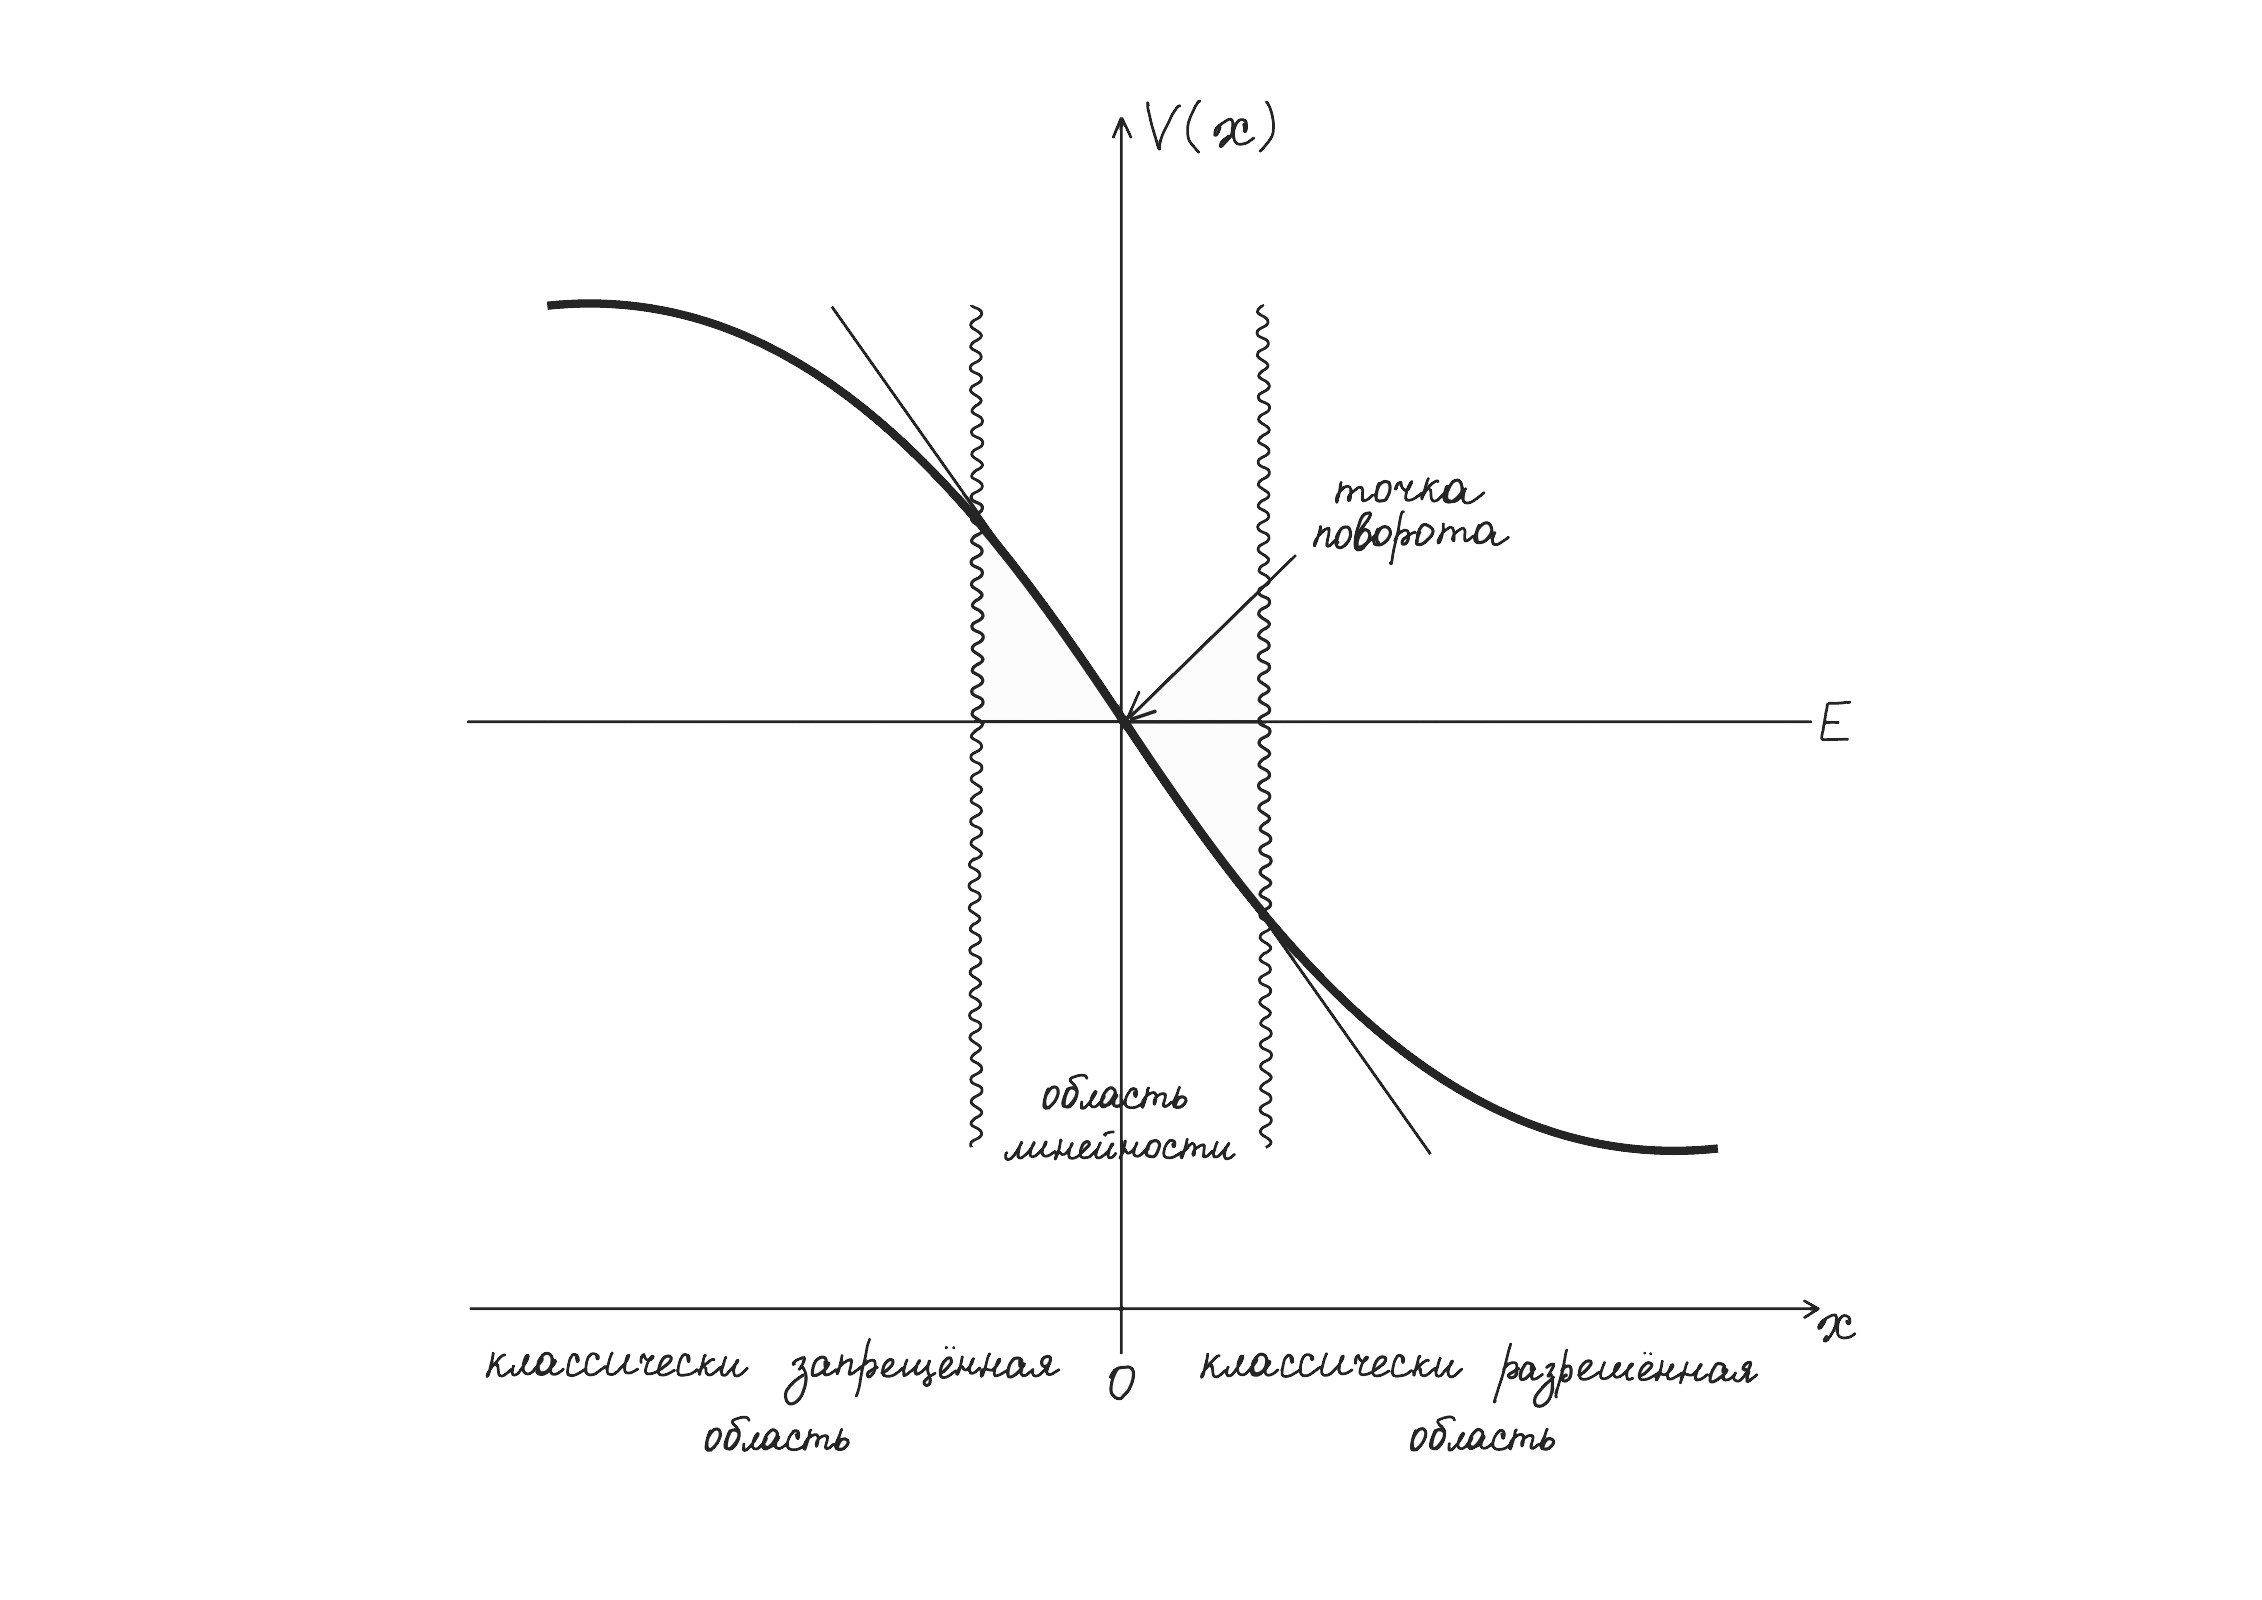
\includegraphics[scale=0.21]{appendix/images/left-turning-point.jpg}
\caption{Потенциальный барьер}
\label{fig C.1}
\end{figure}
Подход будет аналогичным, как и для правой точки. Для начала запишем волновую функцию, коэффициенты которой будем искать:
\[
\psi(x) \simeq 
\begin{cases}
     \frac{1}{\sqrt{|p|}}\left[ Ae^{-\frac{1}{\hbar}\int\limits_x^{0} |p| dx'} \right],\; x < 0;\\
    \frac{1}{\sqrt{p}}\left[ Be^{\frac{i}{\hbar}\int\limits_{0}^{x} p dx'} + Ce^{-\frac{i}{\hbar}\int\limits_{0}^{x} p dx'} \right],\; 0 < x.
\end{cases}
\]
Запишем линеаризованный потенциал (обращаю внимание на то, что в этот раз первая производная будет отрицательной, так как потенциал убывает) как $V(x) \approx E + V'(0)x$. Тогда уравнение Шрёдингера будет иметь следующий вид:
\[
    \frac{d^2\psi_T}{d\psi_T^2} = -\alpha^3 x\psi_p, \quad \alpha = \left( \frac{2m|V'(0)|}{\hbar^2} \right)^{1/3}
\]
Решением этого дифференциального уравнения опять будут функции Эйри:
\[
\psi_T(x) = aAi(-\alpha x) + bBi(-\alpha x)
\]
Посчитаем импульс:
\[
p \simeq \sqrt{2m|V'(0)|x} = \hbar\alpha^{3/2}\sqrt{x}
\]
Подставим импульс в интеграл для классически запрещённой области:
\[
\int\limits_{x}^{0} |p| dx' = \hbar\alpha^{3/2} \int\limits_{x}^{0}\sqrt{-x'} dx' = \frac{2}{3}\hbar(-\alpha x)^{3/2}
\]
Запишем волновую функцию в той же области с полученным значением интеграла:
\[
\psi(x) \simeq \frac{A}{\hbar^{1/2}\alpha^{3/4}(-x)^{1/4}} e^{-\frac{2}{3}(-\alpha x)^{3/2}}
\]
Воспользуемся аппроксимацией для больших значений $-\alpha x \gg 0$:
\[
\psi_T \approx \frac{a}{2\pi^{1/2}(-\alpha x)^{1/4}}e^{-\frac{2}{3}(-\alpha x)^{3/2}} + \frac{b}{\pi^{1/2}(-\alpha x)^{1/4}}e^{\frac{2}{3}(-\alpha x)^{3/2}}
\]
Сравнивая две функции, получим:
\[
a = 2A\sqrt{\frac{\pi}{\alpha\hbar}},\; b = 0
\]

Проделаем аналогичные рассуждения для классически разрешенной области:
\begin{gather*}
\int\limits_{0}^{x} p dx' = \hbar\alpha^{3/2} \int\limits_{0}^{x}\sqrt{x'} dx' = \frac{2}{3}\hbar(\alpha x)^{3/2}\; =>\\
=>\; \psi(x) \simeq \frac{1}{\hbar^{1/2}\alpha^{3/4}x^{1/4}}\left[ Be^{i\frac{2}{3}(\alpha x)^{3/2}} + Ce^{-i\frac{2}{3}(\alpha x)^{3/2}} \right]
\end{gather*}
В этот раз воспользуемся аппроксимацией для малых значений $\alpha x \ll 0$:
\[
\psi_T \approx \frac{a}{\pi^{1/2}(\alpha x)^{1/4}}\sin\left[\frac{2}{3}(\alpha x)^{3/2} + \frac{\pi}{4}\right] = \frac{a}{\pi^{1/2}(\alpha x)^{1/4}}\frac{1}{2i}\left[ e^{i\frac{\pi}{4}}e^{i\frac{2}{3}(\alpha x)^{3/2}} - e^{-i\frac{\pi}{4}}e^{-i\frac{2}{3}(\alpha x)^{3/2}} \right].
\]
Опять сравнив две волновые функции, получим:
\[
B = \frac{a}{2i}\sqrt{\frac{\alpha\hbar}{\pi}}e^{i\frac{\pi}{4}},\; C = -\frac{a}{2i}\sqrt{\frac{\alpha\hbar}{\pi}}e^{-i\frac{\pi}{4}}
\]
Подставим ранее полученную a, выраженную через коэффициент A:
\[
B = -ie^{i\frac{\pi}{4}}A,\; C = ie^{-i\frac{\pi}{4}}A
\]
Подставляя эти значения в первоначальную функцию для x>0, получим:
\[
\psi(x) \simeq \frac{-iA}{\sqrt{p}}\left[ e^{\frac{i}{\hbar}\int\limits_{0}^{x} p dx' + i\frac{\pi}{4}} - e^{-\frac{i}{\hbar}\int\limits_{0}^{x} p dx' - i\frac{\pi}{4}} \right] = \frac{2A}{\sqrt{p}}\sin\left[ \frac{1}{\hbar} \int\limits_0^{x}p dx' + \frac{\pi}{4} \right]
\]
Запишем итоговый вид волновой функции для левой точки поворота:
\[
\psi_L(x) \simeq 
\begin{cases}
    \frac{A}{\sqrt{|p|}}e^{-\frac{1}{\hbar} \int\limits_{x}^{x_1} |p|\,dx'},\; \text{при } x < x_1\\
    \frac{2A}{\sqrt{p}}\sin\left[ \frac{1}{\hbar} \int\limits_{x_1}^{x} p\,dx' + \frac{\pi}{4} \right], \; \text{при } x > x_1\\
\end{cases}
\]
\csquare{darklavender}
\newpage
\excersize{Упражнение №C3}{darklavender}
\begin{center}
\textit{Рассмотрите задачу с потенциальным барьером (рисунок \ref{fig C.2}). Найдите волновую функцию. Запишите, какой в этом случае будет коэффициент прохождения $T$}.
\end{center}

\begin{figure}[h!]
\centering
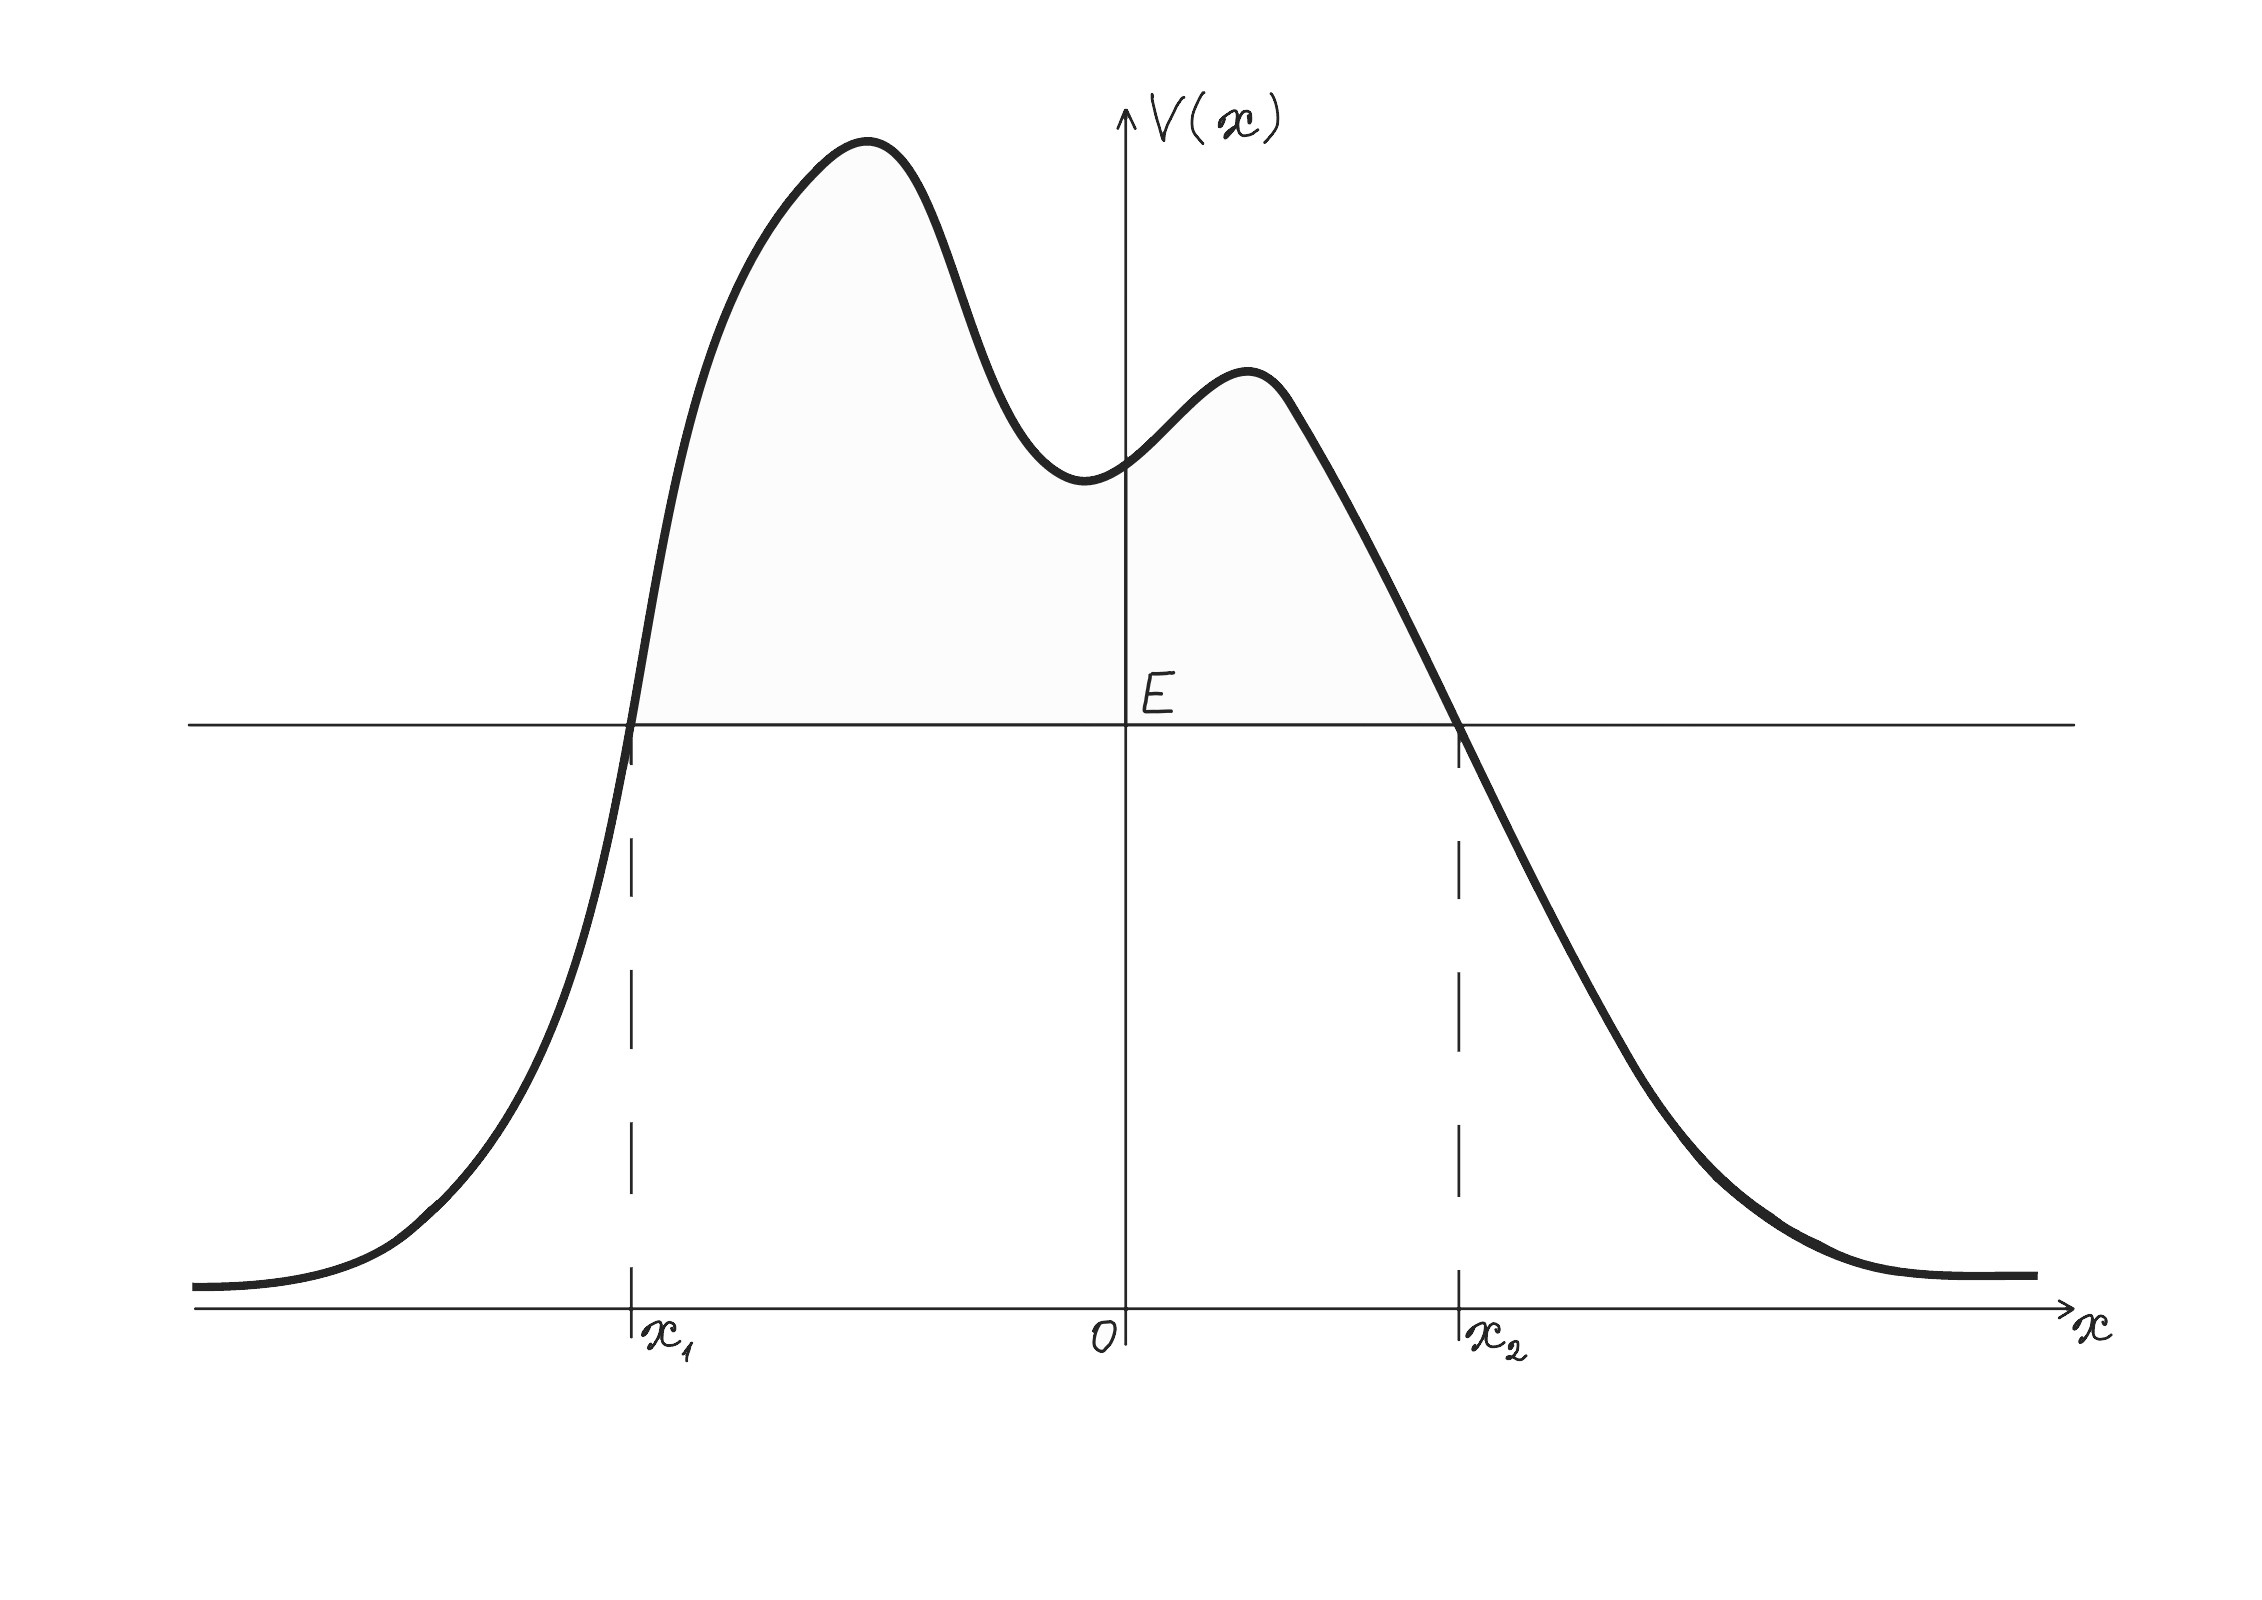
\includegraphics[scale=0.16]{appendix/images/barier.jpg}
\caption{Потенциальный барьер}
\label{fig C.2}
\end{figure}

Запишем общую волновую функцию:
\[
\psi(x) \simeq 
\begin{cases}
    \frac{1}{\sqrt{p}}\left[ Ae^{\frac{i}{\hbar}\int\limits_x^{x_1} p dx'} + Be^{-\frac{i}{\hbar}\int\limits_x^{x_1} p dx'} \right],\; x<x_1;\\
    \frac{1}{\sqrt{|p|}}\left[ Ce^{\frac{1}{\hbar}\int\limits_{x_1}^{x} |p| dx'} + De^{-\frac{1}{\hbar}\int\limits_{x_1}^{x} |p| dx'} \right],\; x_1< x < x_2;\\
    \frac{1}{\sqrt{p}}\left[ Fe^{\frac{i}{\hbar}\int\limits_{x_2}^{x} p dx'}\right],\; x > x_2.
\end{cases}
\]
Внутри барьера запрещённая область, поэтому импульс стоит под модулем. Слева приходит обычная волна и улетает отражённая, поэтому экспоненты две. Справа же только волна, которая прошла сквозь барьер, поэтому слагаемое только одно. 

Для нахождения коэффициентов будем использовать тот же подход, что мы использовали в нахождении волновых функций для точек поворота в потенциальной яме. Тем более, что при аппроксимации функций Эйри получатся те же самые $\psi_T$. Итак, считаем интеграл от импульса, подставляем в волновую функцию для правой области левой точки поворота ($x_1 < x < x_2$), получим:
\[
    \psi(x) \simeq \frac{1}{\hbar^{1/2}\alpha^{3/4}x^{1/4}}\left[ Ce^{\frac{2}{3}(\alpha x)^{3/2}} + De^{-\frac{2}{3}(\alpha x)^{3/2}} \right]
\]
Аппроксимация остаётся такой же:
\[
    \psi_T \approx \frac{a}{2\pi^{1/2}(\alpha x)^{1/4}}e^{-\frac{2}{3}(\alpha x)^{3/2}} + \frac{b}{\pi^{1/2}(-\alpha x)^{1/4}}e^{\frac{2}{3}(-\alpha x)^{3/2}}
\]
Сравнивая, получим:
\[
a = 2D\sqrt{\frac{\pi}{\alpha\hbar}},\; b = C\sqrt{\frac{\pi}{\alpha\hbar}}
\]
Для левой области получим следующие волновые функции:
\begin{align*}
    \psi(x) &\simeq \frac{1}{\hbar^{1/2}\alpha^{3/4}(-x)^{1/4}}\left[ Ae^{i\frac{2}{3}(\alpha x)^{3/2}} + Be^{-i\frac{2}{3}(\alpha x)^{3/2}} \right];\\
    \psi_T(x) &\approx \frac{a}{\pi^{1/2}(\alpha x)^{1/4}}\sin\left[\frac{2}{3}(\alpha x)^{3/2} + \frac{\pi}{4}\right] + \frac{b}{\pi^{1/2}(\alpha x)^{1/4}}\cos\left[\frac{2}{3}(\alpha x)^{3/2} + \frac{\pi}{4}\right] = \\ 
    & = \frac{a}{2\pi^{1/2}(-\alpha x)^{1/4}}\left[ (-ia + b)e^{i\frac{\pi}{4}}e^{i\frac{2}{3}(\alpha x)^{3/2}} + (ia+b)e^{-i\frac{\pi}{4}}e^{-i\frac{2}{3}(\alpha x)^{3/2}} \right].
\end{align*}
Вновь сравнивая, получим:
\[
A = \sqrt{\frac{\hbar\alpha}{\pi}}\left( \frac{-ia + b}{2} \right)e^{i\frac{\pi}{4}},\; B = \sqrt{\frac{\hbar\alpha}{\pi}}\left( \frac{ia + b}{2} \right)e^{-i\frac{\pi}{4}}
\]
Подставим ранее полученные значения коэффициентов a и b:
\[
    A = \left( \frac{C}{2} - iD \right)e^{i\frac{\pi}{4}}, \; B = \left( \frac{C}{2} + iD \right)e^{-i\frac{\pi}{4}}
\]

Для правой точки поворота, для начала, перепишем волновую функцию для запрещённой области в следующем виде:
\[
\psi(x) \simeq \frac{1}{\sqrt{|p|}} \left[ Ce^{\frac{1}{\hbar}\int\limits_{x_1}^{x_2} |p| dx + \frac{1}{\hbar}\int\limits_{x_2}^{x} |p| dx'} + De^{-\frac{1}{\hbar}\int\limits_{x_1}^{x_2} |p| dx - \frac{1}{\hbar}\int\limits_{x_2}^{x} |p| dx'} \right]
\]

Введём новые обозначения. Пусть $\gamma = \frac{1}{\hbar}\int\limits_{x_1}^{x_2} |p| dx$, $C' = De^{-\gamma}$ и $D' = Ce^{\gamma}$ и сместим ноль в правую точку поворота. Тогда волновая функция будет иметь следующий вид:
\[
   \psi(x) \simeq 
   \begin{cases}
   \frac{1}{\sqrt{|p|}}\left[ C'e^{\frac{1}{\hbar}\int\limits_{x}^{0} |p| dx'} + D'e^{-\frac{1}{\hbar}\int\limits_{x}^{0} |p| dx'} \right],\; x < 0;\\
   \frac{1}{\sqrt{p}}\left[ Fe^{\frac{i}{\hbar}\int\limits_{0}^{x} p dx'} \right],\; x > 0
   \end{cases}
\]
Далее делаем всё по аналогии:
\[
\begin{cases}
    \psi(x) \simeq \frac{1}{\hbar^{1/2}\alpha^{3/4}(-x)^{1/4}}\left[ C'e^{\frac{2}{3}(\alpha x)^{3/2}} + D'e^{-\frac{2}{3}(\alpha x)^{3/2}} \right]\\
    \psi_T \approx \frac{a}{2\pi^{1/2}(-\alpha x)^{1/4}}e^{-\frac{2}{3}(-\alpha x)^{3/2}} + \frac{b}{\pi^{1/2}(-\alpha x)^{1/4}}e^{\frac{2}{3}(-\alpha x)^{3/2}}
\end{cases}
 \; => \;
 \begin{cases}
     a = 2\sqrt{\frac{\pi}{\hbar\alpha}}D'\\
     b = \sqrt{\frac{\pi}{\hbar\alpha}}C'
 \end{cases}
\]
Рассмотрим классически разрешённую область:
\[
\begin{cases}
    \psi(x) \simeq \frac{1}{\hbar^{1/2}\alpha^{3/4}x^{1/4}}Fe^{i\frac{2}{3}(\alpha x)^{3/2}}\\
    \psi_T \approx \frac{a}{2\pi^{1/2}(\alpha x)^{1/4}}\left[ (-ia + b)e^{i\frac{\pi}{4}}e^{i\frac{2}{3}(\alpha x)^{3/2}} + (ia+b)e^{-i\frac{\pi}{4}}e^{-i\frac{2}{3}(\alpha x)^{3/2}} \right]
\end{cases}
 \; => \; (ia + b) = 0.
\]
Тогда, выразим коэффициенты $a$ и $b$ через $F$:
\[
F = \sqrt{\frac{\hbar\alpha}{\pi}}\left( \frac{-ia + b}{2} \right)e^{i\frac{\pi}{4}}\; => \; b = \sqrt{\frac{\pi}{\hbar\alpha}} e^{-i\frac{\pi}{4}}F, \; a = i\sqrt{\frac{\pi}{\hbar\alpha}} e^{-i\frac{\pi}{4}}F
\]
Найдём связь коэффициентов $C$ и $D$ с коэффициентом $F$:
\[
\begin{cases}
    C' = e^{-i\frac{\pi}{4}}F\\
    D' = \frac{i}{2}e^{-i\frac{\pi}{4}}F
\end{cases}
\; => \;
\begin{cases}
    D = e^{-i\frac{\pi}{4}}Fe^{\gamma}\\
    C = \frac{i}{2}e^{-i\frac{\pi}{4}}Fe^{-\gamma}
\end{cases}
\]
Подставив их в формулу для $A$, получим нужную нам связь между $A$ и $F$:
\[
A = \left( \frac{C}{2} - iD \right)e^{i\frac{\pi}{4}} = i\left( \frac{e^{-\gamma}}{4} - e^{\gamma} \right)F
\]
Коэффициент прохождения есть отношение коэффициента прошедшей к коэффициенту падающей волны $T \frac{|F|^2}{|A|^2}$. Найдём его в нашей задаче:
\[
T = \frac{1}{(e^{\gamma} - e^{-\gamma}/4)^2} = \frac{e^{-2\gamma}}{[1-(e^{-\frac{\gamma}{2}})^2]^2}
\]
При $\gamma \gg 1$ знаменатель близок к 1 и тогда можно записать коэффициент пропускания как
\[
T = e^{-2\gamma}
\]
\csquare{darklavender}

\excersize{Упражнение №C4}{darklavender}
\begin{center}
\textit{Частица массой m с энергией E ``заперта'' в области $r<r_1$, где $U(r) = -U_0$. При $r > r_1$ потенциал имеет вид:}
\[
U(r) = \frac{2Ze^2}{r}; \; E \ll \frac{2Ze^2}{r_1}
\]
\textit{Воспользовавшись квазиклассическим приближением, найдите коэффициент прохождения сквозь барьер.}
\end{center}

\begin{figure}[h!]
\centering
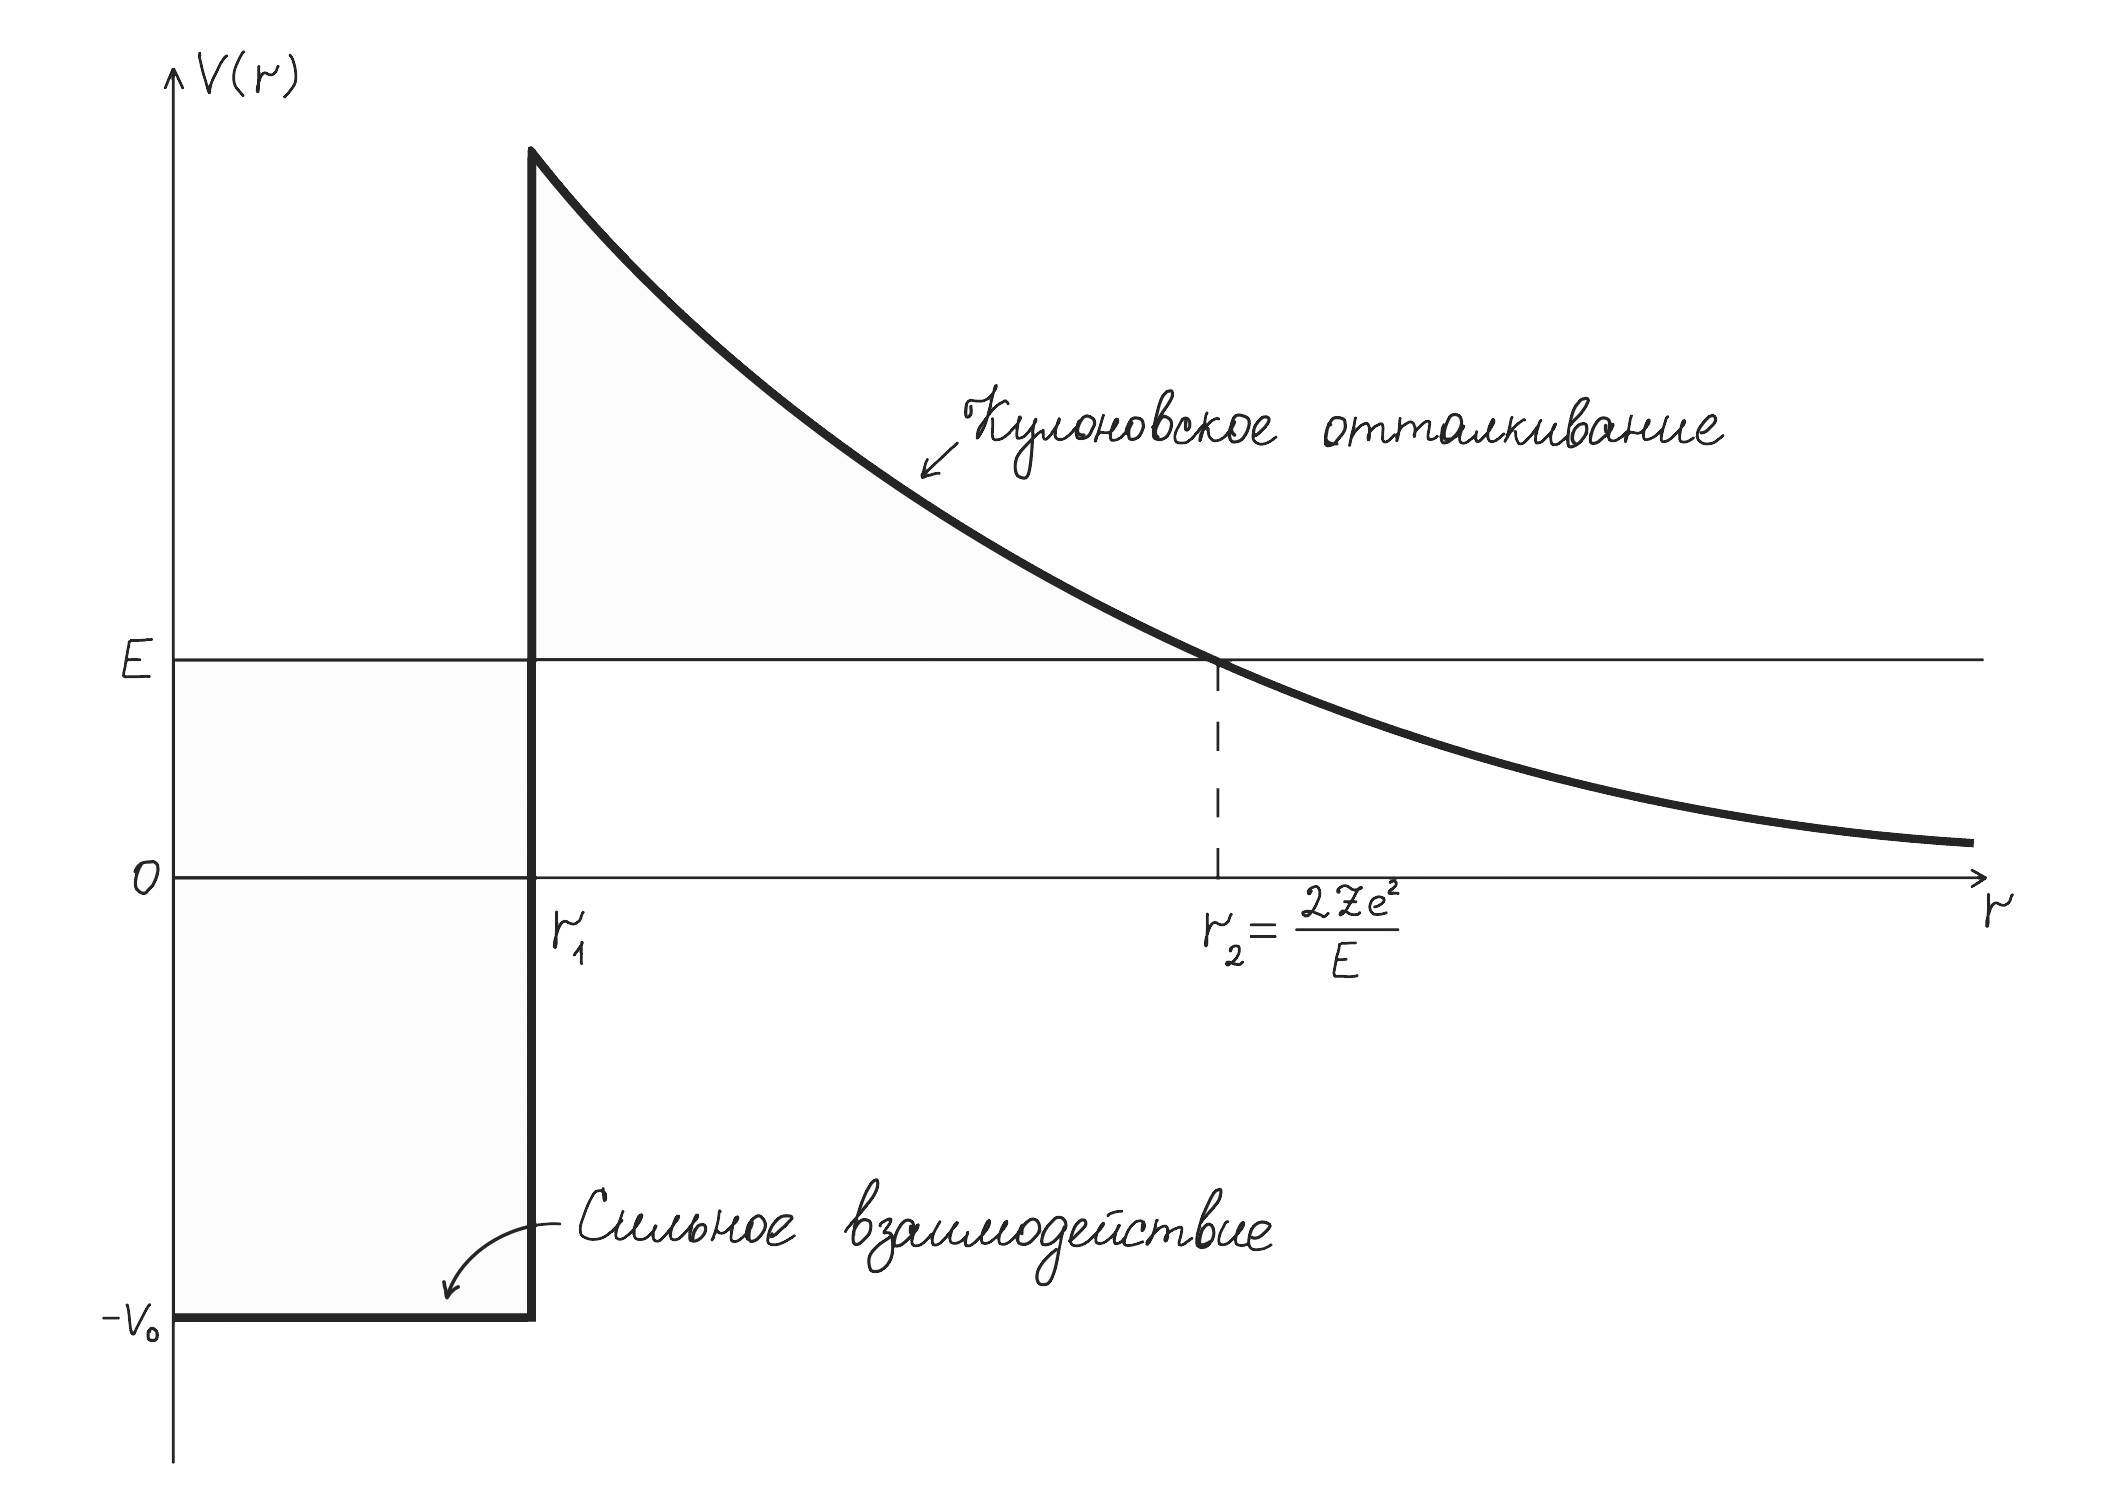
\includegraphics[scale=0.2]{appendix/images/alpha-decay.jpg}
\caption{Модель альфа излучения}
\label{fig C.3}
\end{figure}

Из предыдущей задачи мы знаем, что коэффициент прохождения можно выразить как $T = e^{-2\gamma}$, где $\gamma = \int_{x_1}^{x_2}p dx$. Определим правую точку поворота как $r_2 = 2Ze^2/E$. Посчитаем гамму для нашей задачи:
\begin{align*}
    \gamma & = \frac{1}{\hbar}\int\limits_{r_1}^{r_2}\sqrt{\frac{2Ze^2}{r} - E}dx = \frac{\sqrt{2mE}}{\hbar} \int\limits_{r_1}^{r_2} \sqrt{\frac{r_2}{r} - 1}dx = \\
    &= (r = r_2\sin^2 u) = \frac{\sqrt{2mE}}{\hbar}\left[ r_2\left( \frac{\pi}{2} - \arcsin\sqrt{\frac{r_1}{r_2}} \right) - \sqrt{r_1 (r_2 - r_1)}\right]
\end{align*}
На практике оказывается, что $r_1 \ll r_2$. Тогда $\arcsin (x)\approx x$ и гамма равна
\[
\gamma \simeq \frac{\sqrt{2mE}}{\hbar}\left[ \frac{\pi}{2}r_2 - 2\sqrt{r_1 r_2} \right] = K_1\frac{Z}{\sqrt{E}} - K_2\sqrt{Zr_1},
\]
где $K_1 = \frac{e^2\pi\sqrt{2m}}{\hbar}$ и $K_2 = \frac{4e\sqrt{m}}{\hbar}$. Тогда коэффициент прохождения равен
\[
T = e^{-2\gamma} = e^{2K_2\sqrt{Zr_1} - K_1\frac{2Z}{\sqrt{E}}}
\]
\csquare{darklavender}
    \newpage
    \begin{center}
    \section{Благодарности}
\end{center}

Первоначально эти записи подразумевались как конспекты, используя которые мне было бы проще рассказывать семинары. В какой-то момент пришло понимание, что эти записи могут стать полноценным самостоятельным учебным пособием, с погружением в теорию, подробным решением задач и красивыми картинками. Сначала задача казалась неподъёмной. Оказалось, что это вполне посильно. Всё, что нужно, это люди, которые смогут помочь и поддержать в самые сложные и не очень моменты. Таким людям и посвящена эта глава.

Первым делом хочу сказать огромное спасибо Хамидуллиной Галие. Если вам понравились рисунки, вы не нашли опечатки в формулах или смогли разобраться, как себя ведёт частица в трёхмерном осцилляторе -- это всё её работа. Помимо того, что она хорошо знает математику и может взять любой интеграл, она так же всегда готова помочь, когда это особенно необходимо. Без неё эта работа не получилось бы такой полноценной и самостоятельной. Не говоря уже о том, что она помогала мне и на моих обычных семинарах. Её по праву можно назвать соавтором как минимум этого пособия.

Когда пишешь такую работу, очень важно сохранять интерес и мотивацию. Это было бы невозможно без очень близкого и важного для меня человека -- Койновой Наталии. Её постоянная поддержка и напоминание о том, насколько важна и интересна эта работа, помогали мне на протяжении всего этапа написания семинаров. Когда я терял веру в себя, именно она помогала мне её найти и снова сесть за рабочий стол. Даже если бы я написал эту работу сам, без неё она бы никогда не вышла. Помимо психологической поддержки, Наташа идеально знает русский язык. Поэтому, она выступала в роли редактора этих семинаров. Надеюсь, от неё не ускользнула ни одна моя ошибка. Спасибо ей за всё.

Так же хочется сказать спасибо моему самому первому набору: Коле, Глебу, Алёне, Тимуру, Саше и Галие (уже упомянутой выше). Они смогли подарить мне уверенность в том, что эта работа действительно кому-то нужна и может помочь при решении домашнего задания, на сдачах и на экзамене. Самое важное, что они доверились мне, и пошли на ещё совсем сырые семинары. Благодаря им они стали гораздо лучше.

Последнюю благодарность я бы хотел выразить своему преподавателю по статистической физике -- Суровцеву Евгению Владимировичу. И хоть мы встретились с ним, когда я уже начал рассказывать квантовую механику, он послужил для меня преподавательским ориентиром. Его очень доброе, местами ироничное отношение к студентам в совокупности с глубоким знанием предмета и большим желанием его понятно объяснить делают из него показательного лектора и семинариста. Если когда-нибудь я стану преподавателем, именно он будет той планкой, на которую я буду равняться. 
    \newpage
\end{document}

% TODO:
% 1) написать предисловие/титульник
% 2) написать приложение B
% 3) проверить 1 (+--), 2, 3, 4, 5, 6, 7, 8, 9, 10, 11 семинар. :*
